\documentclass[12pt,a4paper,oneside,openright]{book}
\usepackage{lmodern}
\usepackage{amssymb,amsmath}
\usepackage{ifxetex,ifluatex}
\usepackage{fixltx2e} % provides \textsubscript
\ifnum 0\ifxetex 1\fi\ifluatex 1\fi=0 % if pdftex
  \usepackage[T1]{fontenc}
  \usepackage[utf8]{inputenc}
\else % if luatex or xelatex
  \ifxetex
    \usepackage{mathspec}
    \usepackage{xltxtra,xunicode}
  \else
    \usepackage{fontspec}
  \fi
  \defaultfontfeatures{Mapping=tex-text,Scale=MatchLowercase}
  \newcommand{\euro}{€}
\fi
% use upquote if available, for straight quotes in verbatim environments
\IfFileExists{upquote.sty}{\usepackage{upquote}}{}
% use microtype if available
\IfFileExists{microtype.sty}{%
\usepackage{microtype}
\UseMicrotypeSet[protrusion]{basicmath} % disable protrusion for tt fonts
}{}
\ifxetex
  \usepackage[setpagesize=false, % page size defined by xetex
              unicode=false, % unicode breaks when used with xetex
              xetex]{hyperref}
\else
  \usepackage[unicode=true]{hyperref}
\fi
\hypersetup{breaklinks=true,
            bookmarks=true,
            pdfauthor={},
            pdftitle={},
            colorlinks=true,
            citecolor=blue,
            urlcolor=blue,
            linkcolor=magenta,
            pdfborder={0 0 0}}
\urlstyle{same}  % don't use monospace font for urls
\usepackage{color}
\usepackage{fancyvrb}
\newcommand{\VerbBar}{|}
\newcommand{\VERB}{\Verb[commandchars=\\\{\}]}
\DefineVerbatimEnvironment{Highlighting}{Verbatim}{commandchars=\\\{\}}
% Add ',fontsize=\small' for more characters per line
\usepackage{framed}
\definecolor{shadecolor}{RGB}{248,248,248}
\newenvironment{Shaded}{\begin{snugshade}}{\end{snugshade}}
\newcommand{\KeywordTok}[1]{\textcolor[rgb]{0.13,0.29,0.53}{\textbf{{#1}}}}
\newcommand{\DataTypeTok}[1]{\textcolor[rgb]{0.13,0.29,0.53}{{#1}}}
\newcommand{\DecValTok}[1]{\textcolor[rgb]{0.00,0.00,0.81}{{#1}}}
\newcommand{\BaseNTok}[1]{\textcolor[rgb]{0.00,0.00,0.81}{{#1}}}
\newcommand{\FloatTok}[1]{\textcolor[rgb]{0.00,0.00,0.81}{{#1}}}
\newcommand{\ConstantTok}[1]{\textcolor[rgb]{0.00,0.00,0.00}{{#1}}}
\newcommand{\CharTok}[1]{\textcolor[rgb]{0.31,0.60,0.02}{{#1}}}
\newcommand{\SpecialCharTok}[1]{\textcolor[rgb]{0.00,0.00,0.00}{{#1}}}
\newcommand{\StringTok}[1]{\textcolor[rgb]{0.31,0.60,0.02}{{#1}}}
\newcommand{\VerbatimStringTok}[1]{\textcolor[rgb]{0.31,0.60,0.02}{{#1}}}
\newcommand{\SpecialStringTok}[1]{\textcolor[rgb]{0.31,0.60,0.02}{{#1}}}
\newcommand{\ImportTok}[1]{{#1}}
\newcommand{\CommentTok}[1]{\textcolor[rgb]{0.56,0.35,0.01}{\textit{{#1}}}}
\newcommand{\DocumentationTok}[1]{\textcolor[rgb]{0.56,0.35,0.01}{\textbf{\textit{{#1}}}}}
\newcommand{\AnnotationTok}[1]{\textcolor[rgb]{0.56,0.35,0.01}{\textbf{\textit{{#1}}}}}
\newcommand{\CommentVarTok}[1]{\textcolor[rgb]{0.56,0.35,0.01}{\textbf{\textit{{#1}}}}}
\newcommand{\OtherTok}[1]{\textcolor[rgb]{0.56,0.35,0.01}{{#1}}}
\newcommand{\FunctionTok}[1]{\textcolor[rgb]{0.00,0.00,0.00}{{#1}}}
\newcommand{\VariableTok}[1]{\textcolor[rgb]{0.00,0.00,0.00}{{#1}}}
\newcommand{\ControlFlowTok}[1]{\textcolor[rgb]{0.13,0.29,0.53}{\textbf{{#1}}}}
\newcommand{\OperatorTok}[1]{\textcolor[rgb]{0.81,0.36,0.00}{\textbf{{#1}}}}
\newcommand{\BuiltInTok}[1]{{#1}}
\newcommand{\ExtensionTok}[1]{{#1}}
\newcommand{\PreprocessorTok}[1]{\textcolor[rgb]{0.56,0.35,0.01}{\textit{{#1}}}}
\newcommand{\AttributeTok}[1]{\textcolor[rgb]{0.77,0.63,0.00}{{#1}}}
\newcommand{\RegionMarkerTok}[1]{{#1}}
\newcommand{\InformationTok}[1]{\textcolor[rgb]{0.56,0.35,0.01}{\textbf{\textit{{#1}}}}}
\newcommand{\WarningTok}[1]{\textcolor[rgb]{0.56,0.35,0.01}{\textbf{\textit{{#1}}}}}
\newcommand{\AlertTok}[1]{\textcolor[rgb]{0.94,0.16,0.16}{{#1}}}
\newcommand{\ErrorTok}[1]{\textcolor[rgb]{0.64,0.00,0.00}{\textbf{{#1}}}}
\newcommand{\NormalTok}[1]{{#1}}
\usepackage{longtable,booktabs}
\usepackage{graphicx,grffile}
\makeatletter
\def\maxwidth{\ifdim\Gin@nat@width>\linewidth\linewidth\else\Gin@nat@width\fi}
\def\maxheight{\ifdim\Gin@nat@height>\textheight\textheight\else\Gin@nat@height\fi}
\makeatother
% Scale images if necessary, so that they will not overflow the page
% margins by default, and it is still possible to overwrite the defaults
% using explicit options in \includegraphics[width, height, ...]{}
\setkeys{Gin}{width=\maxwidth,height=\maxheight,keepaspectratio}
\setlength{\parindent}{0pt}
\setlength{\parskip}{6pt plus 2pt minus 1pt}
\setlength{\emergencystretch}{3em}  % prevent overfull lines
\providecommand{\tightlist}{%
  \setlength{\itemsep}{0pt}\setlength{\parskip}{0pt}}
\setcounter{secnumdepth}{0}

\date{}
% Table of contents formatting
\renewcommand{\contentsname}{Table of Contents}
\setcounter{tocdepth}{2}

% Headers and page numbering
\usepackage{fancyhdr}
\pagestyle{plain}

% Fonts and typesetting
%\setmainfont{TeX Gyre Pagella}
%\setsansfont{Verdana}

% Set figure legends and captions to be smaller sized sans serif font
\usepackage[font={footnotesize,sf}]{caption}

\usepackage{siunitx}

% Adjust spacing between lines
%\usepackage{setspace}
%\onehalfspacing
%\raggedbottom
%\linespread{1.0}
% Set margins
\usepackage[top=1.25in,bottom=1.25in]{geometry}

% Chapter styling
%\usepackage[grey]{quotchap}
\makeatletter
%\renewcommand*{\chapnumfont}{%
%  \usefont{T1}{\@defaultcnfont}{b}{n}\fontsize{80}{100}\selectfont% %Default: 100/130
%  \color{chaptergrey}%
%}
\makeatother

% Set colour of links to black so that they don't show up when printed
\usepackage{hyperref}
\hypersetup{colorlinks=true, linkcolor=black}

% Tables
\usepackage{booktabs}
\usepackage{threeparttable}
\usepackage{array}
\usepackage{setspace}
\usepackage{afterpage}
\newcolumntype{x}[1]{%
>{\centering\arraybackslash}m{#1}}%

% Allow for long captions and float captions on opposite page of figures
\usepackage[rightFloats, CaptionBefore]{fltpage}

% Don't let floats cross subsections
\usepackage[section,subsection]{extraplaceins}

\usepackage{multicol}
\newcommand{\columnsbegin}{\begin{multicols}{2}}
\newcommand{\columnsend}{\end{multicols}}
\newcommand\blankpage{%
    \null
    \thispagestyle{empty}%
    \addtocounter{page}{-1}%
    \newpage}

% Redefines (sub)paragraphs to behave more like sections
\ifx\paragraph\undefined\else
\let\oldparagraph\paragraph
\renewcommand{\paragraph}[1]{\oldparagraph{#1}\mbox{}}
\fi
\ifx\subparagraph\undefined\else
\let\oldsubparagraph\subparagraph
\renewcommand{\subparagraph}[1]{\oldsubparagraph{#1}\mbox{}}
\fi

\begin{document}

\thispagestyle{empty} \vspace*{-1.5cm} {\bfseries
\begin{center}
  \Large
  POLITECNICO DI MILANO\\
  \large
  Scuola di Ingegneria Industriale e dell’Informazione\\
  \normalsize
  Corso di Laurea Magistrale in Ingegneria Informatica\\
  Dipartimento di Elettronica, Informazione e Bioingegneria\\

  \vspace*{0.7cm}
  \begin{figure}[htbp]
    \begin{center}
      
\includegraphics[width=3.5cm]{./figures/logopm}
%   
\psfig{file=./pictures/logopm.jpg,width=3.5cm}
    \end{center}
  \end{figure}
  \vspace*{0.3cm} \LARGE



  \textbf{First-Class Continuations on the Java Virtual Machine: An Implementation within the Kawa Scheme Compiler}\\



  \vspace*{.75truecm}

\end{center}
\vspace*{3.0cm} \large
\begin{flushleft}


  Relatore: Prof. Matteo Pradella \\


\end{flushleft}
\vspace*{1.0cm}
\begin{flushright}


  Tesi di Laurea di:\\ Andrea Bernardini \\ matricola 786244 \\


\end{flushright}
\vspace*{0.5cm}
\begin{center}



  Anno Accademico 2014-2015
\end{center} \clearpage
}

\begin{flushright}
\textit{To my family}
\end{flushright}

\newpage

\frontmatter
\chapter{Abstract}

The widespread diffusion of the Java technology has encouraged the birth
of new programming languages on the Java Virtual Machine, languages that
brings new features to the Java environment, most of which taken from
the functional paradigm. Kawa is an implementation of the programming
language Scheme on the Java Virtual Machine. As a Scheme it provides a
functional style of programming, dynamic typing, and meta-programming
facilities. However, being the Java Virtual Machine devoid of stack
manipulation primitives, Kawa lacks of one of the most peculiar Scheme
features: First-class continuations.

This dissertation describes an implementation of the \texttt{call/cc}
control operator in the Kawa compiler. In particular it shows how the
exception handling feature, common to many programming languages, can be
exploited to implement first-class continuations in an environment
without stack manipulation primitives, and how this can be realised in a
real compiler. This thesis also shows how first-class continuations and
control operators like \texttt{call/cc} can be used to introduce
concurrency features and to implement new control flow constructs in
programming languages.

\chapter{Sommario}

La grande diffusione della tecnologia Java ha favorito la nascita di
nuovi linguaggi di programmazione per la Java Virtual Machine, linguaggi
che offrono nuove funzionalità all'ecosistema Java, la maggior parte dei
quali ispirati dal paradigma di programmazione funzionale. Kawa è una
implementazione del di linguaggio di programmazione Scheme pel la Java
Virtual Machine. Come ogni implementazione di Scheme esso fornisce uno
stile funzionale di programmazione, tipizzazione dinamica, e strumenti
per la metaprogrammazione. Tuttavia, essendo la Java Virtual Machine
priva di primitive per la manipolazione diretta dello stack, Kawa manca
di una delle caratteristiche più peculiari di Scheme: le continuazioni
di prima classe.

Questa tesi descrive un'implementazione dell'operatore di controllo
\texttt{call/cc} all'interno del compilatore Kawa. In particolare si
mostra come la gestione delle eccezioni, comune a molti linguaggi di
programmazione, può essere sfruttata per implementare le continuazioni
di prima classe in un ambiente senza primitive di manipolazione dello
stack, e come questo può essere messo in pratica in un vero compilatore.
Si mostra anche in questa trattazione come le continuazioni di prima
classe e gli operatori di controllo come la \texttt{call/cc} possono
essere usate per introdurre concorrenza e nuovi strutture di controllo
nei linguaggi di programmazione.

\chapter{Acknowledgements}

I would like to thank the people who made this thesis possible.

I would like to thank my supervisor Prof.~Matteo Pradella, for inspiring
me with his course on programming languages, and then for giving me the
opportunity to work on this thesis.

Special thanks are given to Per Bothner, the author and project leader
of Kawa, for guiding me in the world of compiler programming. Without
his help, this thesis would not have been possible.

My deepest gratitude goes to my family, for the continuous support
during these years at university, and to my friends, for making this
years unforgettable.

\afterpage{\blankpage}

\tableofcontents
\listoffigures

\mainmatter

\chapter{Introduction}\label{introduction}

\begin{quote}
\emph{``Programming languages are not just technology, but what
programmers think in. They're half technology and half religion.''}

\begin{flushright}
Paul Graham, Beating the Averages
\end{flushright}
\end{quote}

\section{Context}\label{context}

\subsection{Functional programming}\label{functional-programming}

It is well known that the modern computers are not improving their
performance like in the past decades, because frequency scaling, for
silicon, has reached a limit. For this reason, processors manufacturers
increase the potential productivity of their products by adding cores
{[}\hyperref[ref-TurnConcurrency2015]{1}{]}.

\begin{figure}[htbp]
\centering
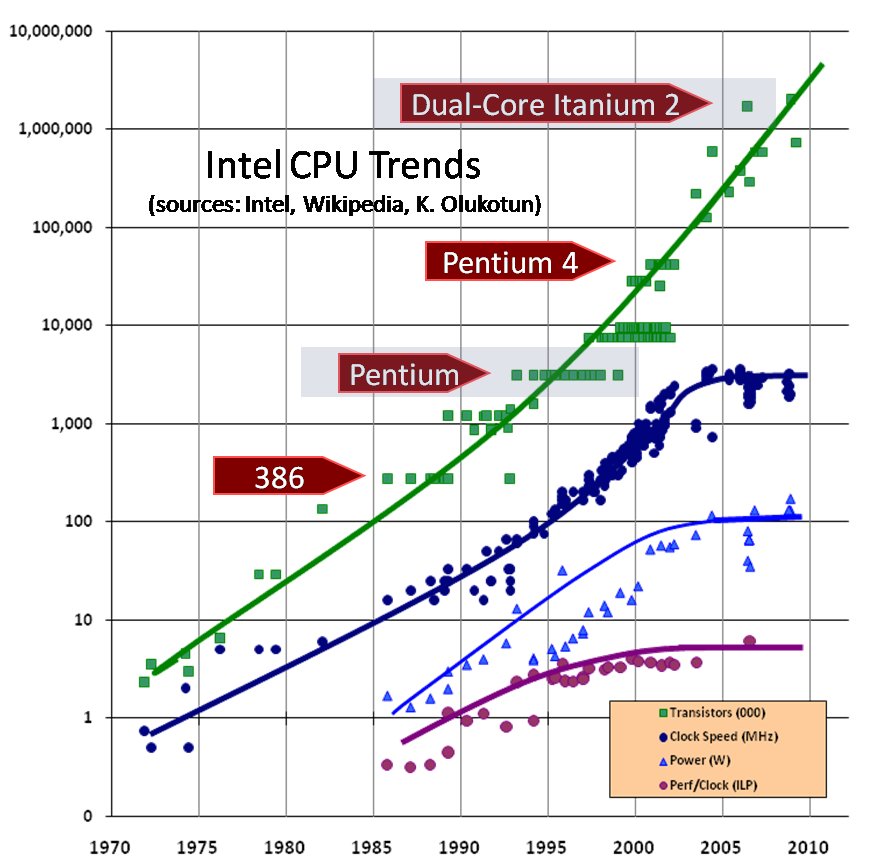
\includegraphics{figures/cpu.png}
\caption{Intel CPU Trends {[}\hyperref[ref-TurnConcurrency2015]{1}{]}
\label{cpu-freq}}
\end{figure}

This implies that to benefit most from this architecture, programs have
to be parallellized. But parallel programming is quite harder than
sequential programming, due to several new challenges it brings.
\emph{Functional programming} (FP) helps to get rid of some of these
challenges, and it has recently risen in importance because it is well
suited for parallel, concurrent and event-driven (or ``reactive'')
programming, thanks to the use of immutable variables and functions
without side effects. The learning curve for functional programming is
often steep, but parallel and concurrent programming with imperative
languages is not intuitive and its learning curve might be even steeper.

Functional programming is often used in synergy with other programming
paradigms, since the world is made of stateful objects, while FP uses a
mainly stateless computation model. FP has ways to model state, but
there is an essential mismatch in a stateless model trying to represent
a stateful world.

However, there are several programming problems in the world that are
easy to map to the FP model. Problems involving concurrency,
parallelism, large data sets and multi-processing.

\subsection{Java}\label{java}

\emph{Java} is a general-purpose programming language that is
concurrent, class-based, object-oriented, and specifically designed to
have as few implementation dependencies as possible. Java code can run
on all platforms that support Java without the need for recompilation.
Java applications are typically compiled to bytecode that can run on any
\emph{Java Virtual Machine} (JVM) regardless of computer architecture.
As of 2015, Java is one of the most popular programming languages in use
{[}\hyperref[ref-TIOBEIndex2015]{2}{]} (see Figures \ref{lang-rank} and
\ref{history-rank}). Java was originally developed by James Gosling at
Sun Microsystems and released in 1995. The language derives much of its
syntax from C and C++, but it has fewer low-level facilities than either
of them {[}\hyperref[ref-JavaWiki2015]{3}{]}.

The reference implementation Java compilers, virtual machines, and class
libraries were open-sourced in May 2007 under the GNU General Public
License.

\begin{figure}[htbp]
\centering
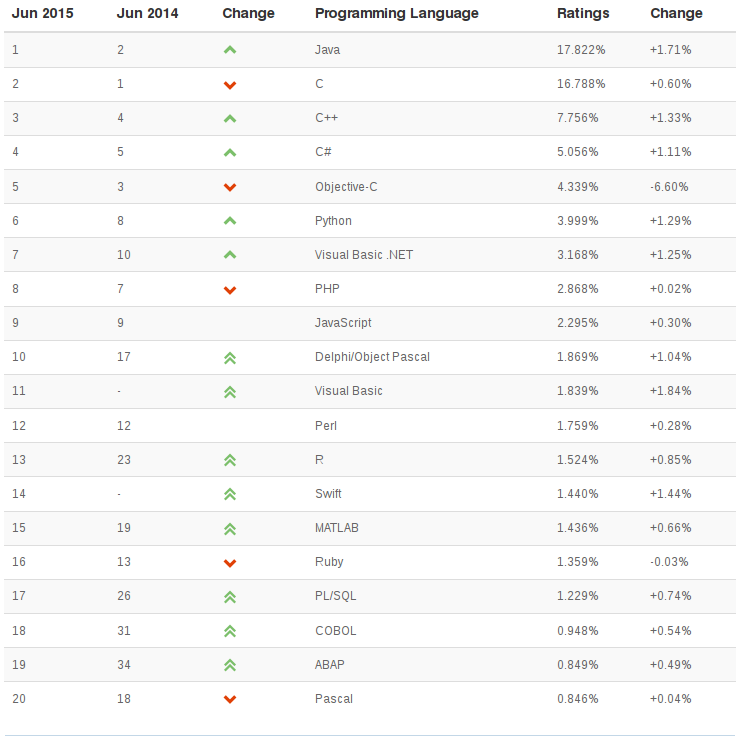
\includegraphics{figures/ranking.png}
\caption{TIOBE Index for June 2015
{[}\hyperref[ref-TIOBEIndex2015]{2}{]} \label{lang-rank}}
\end{figure}

\begin{figure}[htbp]
\centering
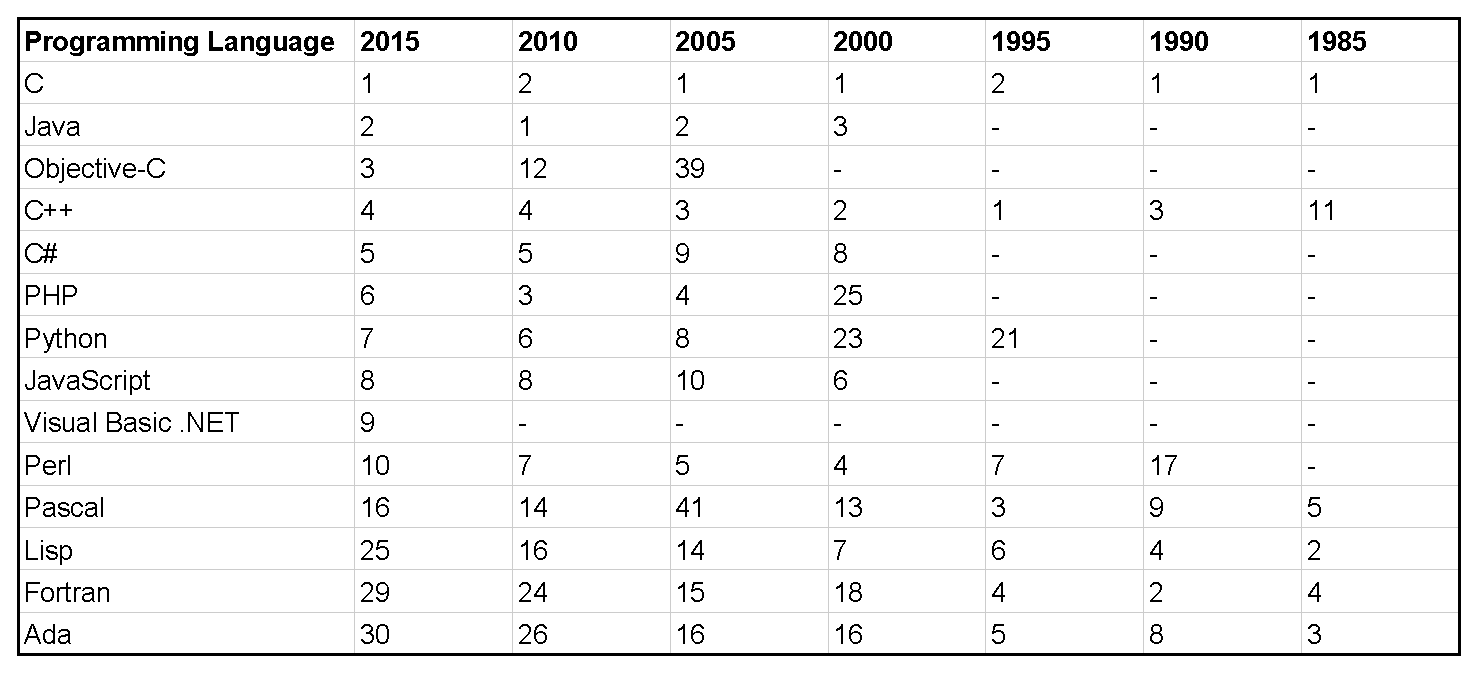
\includegraphics{figures/history_rank.pdf}
\caption{Positions of the top 10 programming languages of many years
back. {[}\hyperref[ref-TIOBEIndex2015]{2}{]} \label{history-rank}}
\end{figure}

\subsubsection{Java 8}\label{java-8}

Starting from release 8, Java supports aspects of functional
programming. Two core concepts introduced in Java 8 are \emph{lambda
expressions} and \emph{functional interfaces}
{[}\hyperref[ref-OracleLambda2015]{4}{]}.

A lambda expression is an anonymous function that can be declared with a
comma separated list of the formal parameters enclosed in parentheses,
an arrow token (-\textgreater{}), and a body. Data types of the
parameters can always be omitted, as can the parentheses if there is
only one parameter. The body can consist of a single statement or a
statement block.

Syntax:

\begin{Shaded}
\begin{Highlighting}[]
    \NormalTok{(arg1, arg2...) -> \{ body \}}

    \NormalTok{(type1 arg1, type2 arg2...) -> \{ body \}}
\end{Highlighting}
\end{Shaded}

Examples:

\begin{Shaded}
\begin{Highlighting}[]
    \NormalTok{(}\DataTypeTok{int} \NormalTok{x, }\DataTypeTok{int} \NormalTok{y) -> x + y}

    \NormalTok{() -> }\DecValTok{42}

    \NormalTok{(String s) -> \{ System.}\FunctionTok{out}\NormalTok{.}\FunctionTok{println}\NormalTok{(s); \}}

    \NormalTok{() -> \{ }\KeywordTok{return} \FloatTok{2.7182} \NormalTok{\};}
\end{Highlighting}
\end{Shaded}

In Java, lambda expressions are represented as objects, and so they must
be bound to a particular object type known as a functional interface. A
functional interface is an interface that defines exactly one abstract
method. An extremely valuable property of functional interfaces is that
they can be instantiated using lambdas.

An example of a functional interface is \texttt{java.lang.Runnable}. It
has only one method void \texttt{run()} declared. Before Java 8,
anonymous inner classes were used to instantiate objects of functional
interface. With Lambda expressions, this can be simplified.

Each lambda expression can be implicitly assigned to one functional
interface. For example we can create \texttt{Runnable} interface's
reference from lambda expression like below:

\begin{Shaded}
\begin{Highlighting}[]
    \NormalTok{Runnable r = () -> System.}\FunctionTok{out}\NormalTok{.}\FunctionTok{println}\NormalTok{(}\StringTok{"running"}\NormalTok{);}
\end{Highlighting}
\end{Shaded}

This type of conversion is automatically handled by the compiler when we
dont specify the functional interface. For example:

\begin{Shaded}
\begin{Highlighting}[]
    \KeywordTok{new} \NormalTok{Thread(}
        \NormalTok{() -> System.}\FunctionTok{out}\NormalTok{.}\FunctionTok{println}\NormalTok{(}\StringTok{"running"}\NormalTok{)}
    \NormalTok{).}\FunctionTok{start}\NormalTok{();}
\end{Highlighting}
\end{Shaded}

In above code, compiler automatically deduced that lambda expression can
be casted to Runnable interface from \texttt{Thread} class's constructor
signature \texttt{public\ Thread(Runnable\ r)\ \{\ \}}.

Few examples of lambda expressions and their functional interface:

\begin{Shaded}
\begin{Highlighting}[]
    \NormalTok{Consumer<Integer>  c = (}\DataTypeTok{int} \NormalTok{x) -> \{ System.}\FunctionTok{out}\NormalTok{.}\FunctionTok{println}\NormalTok{(x) \};}

    \NormalTok{BiConsumer<Integer, String> b = (Integer x, String y)}
                                      \NormalTok{-> System.}\FunctionTok{out}\NormalTok{.}\FunctionTok{println}\NormalTok{(x + y);}

    \NormalTok{Predicate<String> p = (String s) -> \{ s == }\KeywordTok{null} \NormalTok{\};}
\end{Highlighting}
\end{Shaded}

With the addition of Lambda expressions to arrays operations, Java
introduced a key concept into the language of \emph{internal iteration}.
Using that paradigm, the actual iteration over a collection on which a
Lambda function is applied is now carried out by the core library itself
{[}\hyperref[ref-WhyLambda2013]{5}{]}. An relevant possibility opened by
this design pattern is to enable operations carried out on long arrays
(such as sorting, filtering and mapping) to be carried out in parallel
by the framework. For example:

\begin{Shaded}
\begin{Highlighting}[]
    \NormalTok{List<Integer> numbers = Arrays.}\FunctionTok{asList}\NormalTok{(}\DecValTok{1}\NormalTok{, }\DecValTok{2}\NormalTok{, }\DecValTok{3}\NormalTok{, }\DecValTok{4}\NormalTok{, }\DecValTok{5}\NormalTok{, }\DecValTok{6}\NormalTok{);}

    \CommentTok{// old way}
    \KeywordTok{for} \NormalTok{(}\DataTypeTok{int} \NormalTok{number : numbers) \{}
        \NormalTok{System.}\FunctionTok{out}\NormalTok{.}\FunctionTok{println}\NormalTok{(number);}
    \NormalTok{\}}

    \CommentTok{// new way}
    \NormalTok{numbers.}\FunctionTok{forEach}\NormalTok{(value -> System.}\FunctionTok{out}\NormalTok{.}\FunctionTok{println}\NormalTok{(value));}
\end{Highlighting}
\end{Shaded}

In Java 8 it is also possible to reference both a static and an instance
method using the new \texttt{::} operator:

\begin{Shaded}
\begin{Highlighting}[]
    \NormalTok{numbers.}\FunctionTok{forEach}\NormalTok{(System.}\FunctionTok{out}\NormalTok{::println);}
\end{Highlighting}
\end{Shaded}

Passing a lambda expression to another function allows to pass not only
values but also behaviours and this enables to project more generic,
flexible and reusable API. For instance declaring the following method:

\begin{Shaded}
\begin{Highlighting}[]
    \KeywordTok{public} \DataTypeTok{void} \FunctionTok{evaluate}\NormalTok{(List<integer> list,}
                         \NormalTok{Predicate<integer> predicate) \{}
        \KeywordTok{for}\NormalTok{(Integer n: list)  \{}
            \KeywordTok{if}\NormalTok{(predicate.}\FunctionTok{test}\NormalTok{(n)) \{}
                \NormalTok{System.}\FunctionTok{out}\NormalTok{.}\FunctionTok{println}\NormalTok{(n + }\StringTok{" "}\NormalTok{);}
            \NormalTok{\}}
        \NormalTok{\}}
    \NormalTok{\}}
\end{Highlighting}
\end{Shaded}

we can use the \texttt{Predicate} functional interface to create a test
and print the elements that pass the test:

\begin{Shaded}
\begin{Highlighting}[]
    \NormalTok{System.}\FunctionTok{out}\NormalTok{.}\FunctionTok{println}\NormalTok{(}\StringTok{"Print all numbers:"}\NormalTok{);}
    \FunctionTok{evaluate}\NormalTok{(numbers, (n)->}\KeywordTok{true}\NormalTok{);}

    \NormalTok{System.}\FunctionTok{out}\NormalTok{.}\FunctionTok{println}\NormalTok{(}\StringTok{"Print even numbers:"}\NormalTok{);}
    \FunctionTok{evaluate}\NormalTok{(numbers, (n)-> n%}\DecValTok{2} \NormalTok{== }\DecValTok{0} \NormalTok{);}

    \NormalTok{System.}\FunctionTok{out}\NormalTok{.}\FunctionTok{println}\NormalTok{(}\StringTok{"Print odd numbers:"}\NormalTok{);}
    \FunctionTok{evaluate}\NormalTok{(numbers, (n)-> n%}\DecValTok{2} \NormalTok{== }\DecValTok{1} \NormalTok{);}
\end{Highlighting}
\end{Shaded}

Java 8 brings to developers another interesting feature from functional
programming: \emph{Streams}, that is, lazy \emph{evaluation}. Streams
are a new abstraction that allows to process data in a declarative way:

\begin{Shaded}
\begin{Highlighting}[]
    \NormalTok{System.}\FunctionTok{out}\NormalTok{.}\FunctionTok{println}\NormalTok{(}
        \NormalTok{numbers.}\FunctionTok{stream}\NormalTok{()}
            \NormalTok{.}\FunctionTok{filter}\NormalTok{(Lazy::isEven)}
            \NormalTok{.}\FunctionTok{map}\NormalTok{(Lazy::doubleIt)}
            \NormalTok{.}\FunctionTok{filter}\NormalTok{(Lazy::isGreaterThan5)}
            \NormalTok{.}\FunctionTok{findFirst}\NormalTok{()}
    \NormalTok{);}
\end{Highlighting}
\end{Shaded}

You can create a Stream from any Collection by invoking the
\texttt{stream()} method on it. A Stream provides an interface to a
sequenced set of values of a specific element type. However, streams
don't actually store elements; they are computed on demand. They consume
from a data-providing source such as collections, arrays, or I/O
resources and support common operations, such as filter, map, reduce,
find, match, sorted. Furthermore, many stream operations return a stream
themselves. This allows operations to be chained to form a larger
pipeline, enabling also certain optimisations.

\subsubsection{The Java Virtual Machine}\label{the-java-virtual-machine}

A Java Virtual Machine (JVM) is an abstract computing machine defined by
a specification. The specification formally describes what is required
of a JVM implementation. Having a single specification ensures all
implementations are interoperable. A JVM implementation is a software
platform that meets the requirements of the JVM specification in a
compliant and preferably performant manner
{[}\hyperref[ref-JVMWiki2015]{6}{]}.

One of the main goals of Java design is portability, and Java is indeed
platform independent. That is achieved by compiling the Java language
code to an intermediate representation called Java bytecode, instead of
directly to architecture-specific machine code. Java bytecode
instructions are analogous to machine code, but they are intended to be
executed by a virtual machine written specifically for the host
hardware. Moreover, Just-in-Time (JIT) compilers were introduced from an
early stage that compile bytecodes to machine code during runtime. Thus
a JVM is platform dependent, because it must convert Java bytecode into
machine language which depends on the architecture and operating system
being used. End users commonly use a Java Runtime Environment (JRE)
installed on their own machine for standalone Java applications, or in a
web browser for Java applets {[}\hyperref[ref-JavaWiki2015]{3}{]}.

The Oracle Corporation, which owns the Java trademark, distributes the
Java Virtual Machine implementation HotSpot together with an
implementation of the Java Class Library under the name Java Runtime
Environment (JRE).

\subsubsection{JVM based Languages}\label{jvm-based-languages}

The JVM is not only for Java. Several hundred JVM programming languages
are available to be run on it. These languages ultimately compile to
bytecode in class files, which the JVM can then execute.

Some JVM languages include more features than Java and aim to let
developers write code in a more concise way. Features like collection
literals, pattern matching, and a more sophisticated type inference were
the motivation for languages such as Scala, Groovy, Xtend, Ceylon,
Kotlin, and Fantom {[}\hyperref[ref-JVMLang2015]{7}{]}.

Then there are existing languages that were ported to the JVM. Python,
Erlang, Ruby, Scheme and Javascript, for instance, all have an
implementation targeting the JVM (respectively Jython, Erjang, JRuby,
Kawa and Rhino). Another popular language ported to the JVM is Clojure,
a dialect of Lisp with an emphasis on functional and concurrent
programming {[}\hyperref[ref-JVMWiki2015]{6}{]}.

Many less-known JVM languages implement new research ideas, are suited
only for a specific domain, or are just experimental.

\subsection{Scheme}\label{scheme}

\emph{Scheme} is a dialect of the computer programming language Lisp. It
follows a minimalist design philosophy that specifies a small standard
core accompanied by powerful tools for meta-programming.

Scheme was created during the 1970s at the MIT AI Lab by Guy L. Steele
and Gerald Jay Sussman. It was the first dialect of Lisp to choose
lexical scope and the first to require implementations to perform
tail-call optimisation. It was also one of the first programming
languages to support first-class continuations
{[}\hyperref[ref-SchemeWiki2015]{8}{]}.

Scheme is a general-purpose computer programming language. It is a
high-level language, supporting operations on structured data such as
strings, lists, and vectors, as well as operations on more traditional
data such as numbers and characters. Scheme is a fairly simple language
to learn, since it is based on a handful of syntactic forms and semantic
concepts and since the interactive nature of most implementations
encourages experimentation {[}\hyperref[ref-dybvig2009scheme]{9}{]}.

The storage required to hold the contents of an object is dynamically
allocated as necessary and retained until no longer needed, then
automatically deallocated, typically by a garbage collector. Simple
atomic values, such as small integers, characters, booleans, and the
empty list, are represented as primitive types and thus incur no
allocation or deallocation overhead
{[}\hyperref[ref-dybvig2009scheme]{9}{]}.

Scheme is \emph{homoiconic}, i.e, programs share a common representation
with Scheme data structures. As a result, any Scheme program has an
internal representation as a Scheme object. For example, variables and
syntactic keywords correspond to symbols, while structured syntactic
forms correspond to lists. This representation is the basis for the
syntactic extension facilities provided by Scheme for the definition of
new syntactic forms. It also facilitates the implementation of
interpreters, compilers, and other program transformation tools
{[}\hyperref[ref-dybvig2009scheme]{9}{]}.

In Scheme, a procedure definition may appear within another block or
procedure, and the procedure may be invoked at any time thereafter, even
if the enclosing block has completed its execution. To support lexical
scoping, a procedure carries the lexical context (environment) along
with its code.

Furthermore orover, Scheme provides anonymous procedures. Indeed
procedures are first-class data objects like strings or numbers, and
variables are bound to procedures in the same way they are bound to
other objects.

The Scheme language is standardized in the Revised\textsuperscript{n}
Report on the Algorithmic Language Scheme (RnRS), where the
\textsuperscript{n} indicates the revision number. The last report is
R7RS, released in 2013.

\subsubsection{Scheme basics}\label{scheme-basics}

Scheme syntax is essential, it provides a minimal set of special forms:
define, quote, lambda, cond, let/let*

\texttt{define} is used to define new names.

\begin{Shaded}
\begin{Highlighting}[]
    \NormalTok{(}\KeywordTok{define}\FunctionTok{ x }\DecValTok{10}\NormalTok{)}
    \NormalTok{(}\KeywordTok{define}\FunctionTok{ square }\NormalTok{(}\KeywordTok{lambda} \NormalTok{(x) (* x x)))}
\end{Highlighting}
\end{Shaded}

\texttt{quote} prevents the argument to be evaluated as an expression,
returning it as literal data (symbols or lists).

\begin{Shaded}
\begin{Highlighting}[]
    \NormalTok{(quote hi!)           }\KeywordTok{=>} \NormalTok{hi!}
    \NormalTok{(quote (}\DecValTok{1} \DecValTok{2} \DecValTok{3}\NormalTok{))         }\KeywordTok{=>} \NormalTok{(}\DecValTok{1} \DecValTok{2} \DecValTok{3}\NormalTok{)}

    \CommentTok{; the tick-mark ' is syntactic sugar}
    \NormalTok{'(}\DecValTok{1} \DecValTok{2} \NormalTok{foo bar)          }\KeywordTok{=>} \NormalTok{(}\DecValTok{1} \DecValTok{2} \NormalTok{foo bar)}
\end{Highlighting}
\end{Shaded}

\texttt{lambda} is used to create anonymous functions.

\begin{Shaded}
\begin{Highlighting}[]
    \NormalTok{(}\KeywordTok{lambda} \NormalTok{(x) (* x }\DecValTok{10}\NormalTok{)                   }\CommentTok{; anonymous function}
    \NormalTok{(}\KeywordTok{define}\FunctionTok{ times10 }\NormalTok{(}\KeywordTok{lambda} \NormalTok{(x) (* x }\DecValTok{10}\NormalTok{))) }\CommentTok{; named the function now}
\end{Highlighting}
\end{Shaded}

\texttt{cond} is a general conditional.

\begin{Shaded}
\begin{Highlighting}[]
    \NormalTok{(}\KeywordTok{cond}
      \NormalTok{((}\KeywordTok{eq?} \NormalTok{'foo 'bar) 'hello)}
      \NormalTok{((}\KeywordTok{=} \DecValTok{10} \DecValTok{20}\NormalTok{) 'goodbye)}
      \NormalTok{(}\KeywordTok{else} \NormalTok{'sorry))                  }\KeywordTok{=>} \NormalTok{sorry}
\end{Highlighting}
\end{Shaded}

\texttt{let} is used to declare/use temporary variables.

\begin{Shaded}
\begin{Highlighting}[]
    \NormalTok{(}\KeywordTok{let} \NormalTok{((x }\DecValTok{10}\NormalTok{)}
          \NormalTok{(y }\DecValTok{20}\NormalTok{))}
      \NormalTok{(}\KeywordTok{+} \NormalTok{x y))}
\end{Highlighting}
\end{Shaded}

Built-in types are integers, rationals, floats, characters, strings,
booleans, symbols, lists, and vectors. A set of built-in functions we
can use on these types:

\begin{Shaded}
\begin{Highlighting}[]
    \CommentTok{;; arithmetic:  +, -, *, /}
    \CommentTok{;; relational: <, <=, >, >=, =}
    \NormalTok{(}\KeywordTok{+} \DecValTok{1} \DecValTok{2}\NormalTok{)                    }\KeywordTok{=>} \DecValTok{3}
    \NormalTok{(}\KeywordTok{=} \DecValTok{1} \DecValTok{2}\NormalTok{)                    }\KeywordTok{=>} \DecValTok{#f} \CommentTok{; '=' is for numbers}
\end{Highlighting}
\end{Shaded}

Equality and identity tests:

\begin{Shaded}
\begin{Highlighting}[]
    \NormalTok{(}\KeywordTok{eq?} \NormalTok{'hello 'goodbye)      }\KeywordTok{=>} \DecValTok{#f} \CommentTok{; eq? is an identity test}
    \NormalTok{(}\KeywordTok{eq?} \NormalTok{'hello 'hello)        }\KeywordTok{=>} \DecValTok{#t}
    \NormalTok{(}\KeywordTok{eq?} \NormalTok{'(}\DecValTok{1} \DecValTok{2}\NormalTok{) '(}\DecValTok{1} \DecValTok{2}\NormalTok{))        }\KeywordTok{=>} \DecValTok{#f}
    \NormalTok{(}\KeywordTok{define}\FunctionTok{ foo }\NormalTok{'(}\DecValTok{1} \DecValTok{2}\NormalTok{))}
    \NormalTok{(}\KeywordTok{define}\FunctionTok{ bar }\NormalTok{foo)}
    \NormalTok{(}\KeywordTok{eq?} \NormalTok{foo bar)              }\KeywordTok{=>} \DecValTok{#t}
    \NormalTok{(}\KeywordTok{equal?} \NormalTok{foo bar)           }\KeywordTok{=>} \DecValTok{#t} \CommentTok{; equality: they look the same}
    \NormalTok{(}\KeywordTok{equal?} \NormalTok{foo '(}\DecValTok{1} \DecValTok{2}\NormalTok{))        }\KeywordTok{=>} \DecValTok{#t}
\end{Highlighting}
\end{Shaded}

Being a dialect of Lisp, Scheme provides a set of built-in functions for
List manipulation: cons, car, and cdr.

\begin{Shaded}
\begin{Highlighting}[]
    \CommentTok{;; Three equivalent ways to create the list (1 2 3),}
    \CommentTok{;; calling it foo}
    \NormalTok{(}\KeywordTok{define}\FunctionTok{ foo }\NormalTok{'(}\DecValTok{1} \DecValTok{2} \DecValTok{3}\NormalTok{))}
    \NormalTok{(}\KeywordTok{define}\FunctionTok{ foo }\NormalTok{(}\KeywordTok{cons} \DecValTok{1} \NormalTok{(}\KeywordTok{cons} \DecValTok{2} \NormalTok{(}\KeywordTok{cons} \DecValTok{3} \NormalTok{()))))}
    \NormalTok{(}\KeywordTok{define}\FunctionTok{ foo }\NormalTok{(}\KeywordTok{list} \DecValTok{1} \DecValTok{2} \DecValTok{3}\NormalTok{))}

    \CommentTok{;; list precessing}
    \NormalTok{(}\KeywordTok{null?} \NormalTok{'(}\DecValTok{1} \DecValTok{2}\NormalTok{))             }\KeywordTok{=>} \DecValTok{#f}
    \NormalTok{(}\KeywordTok{null?} \NormalTok{())                 }\KeywordTok{=>} \DecValTok{#t}
    \NormalTok{(}\KeywordTok{car} \NormalTok{'(}\DecValTok{1} \DecValTok{2}\NormalTok{))               }\KeywordTok{=>} \DecValTok{1}
    \NormalTok{(}\KeywordTok{cdr} \NormalTok{'(}\DecValTok{1} \DecValTok{2}\NormalTok{))               }\KeywordTok{=>} \NormalTok{(}\DecValTok{2}\NormalTok{)}
\end{Highlighting}
\end{Shaded}

Iteration via recursion:

\begin{Shaded}
\begin{Highlighting}[]
    \CommentTok{;; Exponentiation function x^n}
    \NormalTok{(}\KeywordTok{define}\FunctionTok{ }\NormalTok{(}\KeywordTok{expt} \NormalTok{x n}
      \NormalTok{(}\KeywordTok{if} \NormalTok{(}\KeywordTok{=} \NormalTok{n }\DecValTok{0}\NormalTok{)}
          \DecValTok{1}
          \NormalTok{(* x (}\KeywordTok{expt} \NormalTok{x (}\KeywordTok{-} \NormalTok{n }\DecValTok{1}\NormalTok{))))))}

    \CommentTok{;; List length}
    \NormalTok{(}\KeywordTok{define}\FunctionTok{ }\NormalTok{(}\KeywordTok{length} \NormalTok{lst}
      \NormalTok{(}\KeywordTok{if} \NormalTok{(}\KeywordTok{null?} \NormalTok{lst)}
          \DecValTok{0}
          \NormalTok{(}\KeywordTok{+} \DecValTok{1} \NormalTok{(}\KeywordTok{length} \NormalTok{(}\KeywordTok{cdr} \NormalTok{lst))))))}
\end{Highlighting}
\end{Shaded}

It is straightforward to create and use higher order functions. Indeed
functions are first-class in Scheme, they can be passed as arguments to
other functions:

\begin{Shaded}
\begin{Highlighting}[]
    \NormalTok{(}\KeywordTok{define}\FunctionTok{ compose}
      \NormalTok{(}\KeywordTok{lambda} \NormalTok{(f g x)}
        \NormalTok{(f (g x))))}

    \NormalTok{(compose }\KeywordTok{even?} \NormalTok{(}\KeywordTok{lambda} \NormalTok{(x) (}\KeywordTok{-} \NormalTok{x }\DecValTok{1}\NormalTok{)) }\DecValTok{10}\NormalTok{)   }\KeywordTok{=>} \DecValTok{#f}

    \CommentTok{;; takes a function and applies it to every element of a list}
    \NormalTok{(}\KeywordTok{define}\FunctionTok{ }\NormalTok{(map f lst)}
      \NormalTok{(}\KeywordTok{let} \NormalTok{loop ((newlst lst))}
        \NormalTok{(}\KeywordTok{cond} \NormalTok{((}\KeywordTok{pair?} \NormalTok{newlst)}
          \NormalTok{(}\KeywordTok{cons} \NormalTok{(f (}\KeywordTok{car} \NormalTok{newlst)) (loop (}\KeywordTok{cdr} \NormalTok{newlst))))}
         \NormalTok{((}\KeywordTok{null?} \NormalTok{newlst)}
          \NormalTok{'())}
         \NormalTok{(}\KeywordTok{else}
          \NormalTok{(error }\StringTok{"second argument is not a list:"}  \NormalTok{lst)))))}

    \NormalTok{(map }\KeywordTok{even?} \NormalTok{'(}\DecValTok{1} \DecValTok{2} \DecValTok{3} \DecValTok{4}\NormalTok{))        }\KeywordTok{=>} \NormalTok{(}\DecValTok{#f} \DecValTok{#t} \DecValTok{#f} \DecValTok{#t}\NormalTok{)}
\end{Highlighting}
\end{Shaded}

\subsection{Continuations}\label{continuations}

Computer programs usually control the flow of execution via procedure
calls and returns; a stack of frames is how high-level programming
languages keep track of the point to which each active subroutine should
return control when it finishes executing. However, to solve real-world
problems, procedure call and primitive expressions are not enough. Thus
most high-level programming languages also provide other control-flow
primitives, like conditionals, loops, and exception handling.

Scheme also supports \emph{first-class continuations}. A continuation is
a Scheme function that embodies ``the rest of the computation''. The
continuation of any Scheme expression determines what is to be done with
its value. This continuation is always present, in any language
implementation, since the system is able to continue from each point of
the computation. Scheme provides a mechanism for capturing this
continuation as a closure. The obtained continuation can be used to
continue, or resume, the computation from the point it was captured,
whether or not the computation has previously completed. This is useful
for nonlocal exits in handling exceptions, or in the implementation of
complex control structures such as coroutines or generators
{[}\hyperref[ref-dybvig1987three]{10}{]}.

Considering a computation such as \texttt{(*\ (+\ 2\ 4)\ (+\ 1\ 6))},
there are several continuations involved. The continuation for
\texttt{(+\ 2\ 4)} can be expressed in this way: take this value (6),
keep it aside; now add one and six, take the result and multiply it with
the value we had kept aside; then finish. The continuation for
\texttt{(+\ 1\ 6)} means: take this value, multiply it with the value
(6) that was previously kept aside; then finish. Notice in particular
how the result of \texttt{(+\ 2\ 4)} is part of the continuation of
\texttt{(+\ 1\ 6)}, because it has been calculated and kept aside.
Continuations are not static entities that can be determined at compile
time: they are dynamic objects that are created and invoked during
program execution.

Using the syntactic form \texttt{call-with-current-continuation}
(usually abbreviated \texttt{call/cc}), a program can obtain its own
continuation. This continuation is a Scheme closure that may be invoked
at any time to continue the computation from the point of the
\texttt{call/cc}. It may be invoked before or after the computation
returns; it may be invoked more than one time.\footnote{For more
  explanation and examples on continuations see
  {[}\hyperref[ref-ContByExample2015]{11}--\hyperref[ref-PageCallcc2015]{13}{]}.}

The standard idiom for \texttt{call/cc} has an explicit lambda term as
its argument:

\begin{Shaded}
\begin{Highlighting}[]
    \NormalTok{(}\KeywordTok{call/cc} \NormalTok{(}\KeywordTok{lambda} \NormalTok{(current-continuation)}
      \NormalTok{body))}
\end{Highlighting}
\end{Shaded}

During the execution of the expression body, the variable
current-continuation is bound to the current continuation. If invoked,
current-continuation immediately returns from the call to
\texttt{call/cc}, and \texttt{call/cc} returns whatever value was passed
to current-continuation.

When applied to a function \texttt{f}, \texttt{call/cc} captures and
aborts the entire continuation \texttt{k}, reinstate a copy of
\texttt{k}, and applies \texttt{f} to \texttt{k}.

Consider a first example:

\begin{Shaded}
\begin{Highlighting}[]
    \NormalTok{(}\KeywordTok{call/cc}
      \NormalTok{(}\KeywordTok{lambda} \NormalTok{(k)}
        \NormalTok{(k }\DecValTok{42}\NormalTok{)))}
\end{Highlighting}
\end{Shaded}

This applies \texttt{call/cc} to the function
\texttt{(lambda\ (k)\ (k\ 42))}, which is called with argument
\texttt{k}, the current continuation. Being the body of the function
\texttt{(k\ 42)}, the continuation is thrown the value 42. This makes
the \texttt{call/cc} return the value 42. Hence, the entire expression
evaluates to 42.

Now consider

\begin{Shaded}
\begin{Highlighting}[]
    \NormalTok{(}\KeywordTok{call/cc}
      \NormalTok{(}\KeywordTok{lambda} \NormalTok{(k)}
        \NormalTok{(}\KeywordTok{+} \NormalTok{(k }\DecValTok{42}\NormalTok{) }\DecValTok{100}\NormalTok{)))}
\end{Highlighting}
\end{Shaded}

In this case, the function throws the value 42 to the continuation, but
there is another computation afterwards. That computation has no effect,
because when a continuation is invoked with a value, the program
reinstates the invoked continuation, and the continuation which was
going to take a value \texttt{x} and perform \texttt{(+\ x\ 100)} has
been aborted. The result is still 42.

On the other hand, consider

\begin{Shaded}
\begin{Highlighting}[]
    \NormalTok{(}\KeywordTok{call/cc}
      \NormalTok{(}\KeywordTok{lambda} \NormalTok{(k) }\DecValTok{42}\NormalTok{))}
\end{Highlighting}
\end{Shaded}

Here, the function applied by \texttt{call/cc} does not make use of the
current continuation. It performs a real return, with the value 42.

Actually, although a continuation can be called as a procedure, it is
not a real function, which takes a value and returns another. An invoked
continuation takes a value and does everything that follows to it, never
returning a value to the caller.

As an other example, consider the following code:

\begin{Shaded}
\begin{Highlighting}[]
    \NormalTok{(}\KeywordTok{display}
        \NormalTok{(}\KeywordTok{call/cc} \NormalTok{(}\KeywordTok{lambda} \NormalTok{(k)}
              \NormalTok{(}\KeywordTok{display} \StringTok{"This is executed.\textbackslash{}n"}\NormalTok{)}
              \NormalTok{(k }\StringTok{"Value passed to the continuation.\textbackslash{}n"}\NormalTok{)}
              \NormalTok{(}\KeywordTok{display} \StringTok{"But not this.\textbackslash{}n"}\NormalTok{))))}
\end{Highlighting}
\end{Shaded}

it will display:

\begin{verbatim}
    This is executed.
    Value passed to the continuation.
\end{verbatim}

An interesting feature of first-class continuations is that the
continuation may still be called even after the call to call/cc is
finished. When applied to a value \texttt{v}, a continuation \texttt{k}
aborts its entire execution context, reinstates \texttt{k} as the
current entire continuation, and returns the value \texttt{v} to the
continuations \texttt{k}, which is ``waiting for a value'' in order to
perform some computation with it. In some Scheme implementations, the
value passed to a continuation can be a void one.

For example, the following causes an infinite loop that prints
\texttt{goto\ start} forever:

\begin{Shaded}
\begin{Highlighting}[]
    \NormalTok{(}\KeywordTok{let} \NormalTok{((start }\DecValTok{#f}\NormalTok{))}
      \NormalTok{(}\KeywordTok{if} \NormalTok{(}\KeywordTok{not} \NormalTok{start)}
        \NormalTok{(}\KeywordTok{call/cc} \NormalTok{(}\KeywordTok{lambda} \NormalTok{(cc)}
                   \NormalTok{(set! start cc))))}

      \NormalTok{(}\KeywordTok{display} \StringTok{"goto start\textbackslash{}n"}\NormalTok{)}
      \NormalTok{(start))}
\end{Highlighting}
\end{Shaded}

\subsubsection{Delimited Continuations}\label{delimited-continuations}

Continuations captured by \texttt{call/cc} is the whole continuation
that includes all the future computation. In some cases, we want to
manipulate only a part of computation. This is possible with a kind of
continuations called \emph{delimited} or \emph{composable} continuations
{[}\hyperref[ref-Asai2011]{14}{]}.

A continuation is delimited when it produces an intermediate answer
rather than the final outcome of the entire computation. In other words,
a delimited continuation is a representation of the ``rest of the
computation'' from the current computation up to a designated boundary.
Unlike regular continuations, delimited continuations return a value,
and thus may be reused and composed
{[}\hyperref[ref-kiselyov2007delimited]{15}{]}.

Various operators for delimited continuations have been proposed in the
research literature, such as \texttt{prompt} and \texttt{control},
\texttt{shift} and \texttt{reset}, \texttt{cupto}, \texttt{fcontrol},
and others {[}\hyperref[ref-RacketContinuations2015]{16}{]}. In this
introduction we will consider only the \texttt{shift} and \texttt{reset}
operators.

The \texttt{reset} operator sets the limit for the continuation while
the \texttt{shift} operator captures or reifies the current continuation
up to the innermost enclosing \texttt{reset}. The \texttt{shift}
operator passes the captured continuation to its body, which can invoke,
return or ignore it. Whatever result that \texttt{shift} produces is
provided to the innermost \texttt{reset}, discarding the continuation in
between the \texttt{reset} and \texttt{shift}. The continuation, if
invoked, effectively reinstates the entire computation up to the
\texttt{reset}. When the computation is completed, the result is
returned by the delimited continuation
{[}\hyperref[ref-DelimitedWiki2015]{17}{]}. For example, consider the
following snippet in Scheme:

\begin{Shaded}
\begin{Highlighting}[]
    \NormalTok{(* }\DecValTok{2} \NormalTok{(reset (}\KeywordTok{+} \DecValTok{1} \NormalTok{(shift k (k }\DecValTok{5}\NormalTok{)))))}
\end{Highlighting}
\end{Shaded}

The \texttt{reset} delimits the continuation that \texttt{shift}
captures. When this code is executed, the use of \texttt{shift} will
bind \texttt{k} to the continuation \texttt{(+\ 1\ {[}{]})} where
\texttt{{[}{]}} represents the part of the computation that is to be
filled with a value. This is exactly the code that surrounds the
\texttt{shift} up to the \texttt{reset}. Since the body of
\texttt{shift} immediately invokes the continuation, the previous
expression is equivalent to the following:

\begin{Shaded}
\begin{Highlighting}[]
    \NormalTok{(* }\DecValTok{2} \NormalTok{(}\KeywordTok{+} \DecValTok{1} \DecValTok{5}\NormalTok{))}
\end{Highlighting}
\end{Shaded}

Once the execution of the \texttt{shift}'s body is completed, the
continuation is discarded, and execution restarts outside
\texttt{reset}. For instance:

\begin{Shaded}
\begin{Highlighting}[]
    \NormalTok{(reset (* }\DecValTok{2} \NormalTok{(shift k (k (k }\DecValTok{4}\NormalTok{)))))}
\end{Highlighting}
\end{Shaded}

invokes \texttt{(k\ 4)} first, which produces 8 as result, and then
\texttt{(k\ 8)}, which returns 16. At this point, the \texttt{shift}
expression has terminated, and the rest of the \texttt{reset} expression
is discarded. Therefore, the final result is 16.

\subsection{Kawa}\label{kawa}

\emph{Kawa} is a language framework written in Java that implements an
extended version of the programming language Scheme. It provides a set
of Java classes useful for implementing dynamic languages, such as those
in the Lisp family. Kawa is also an implementation of almost all of R7RS
Scheme (First-class continuations being the major missing feature), and
which compiles Scheme to the bytecode instructions of the JVM
{[}\hyperref[ref-Kawa2015]{18}{]}. The author and project leader of Kawa
is Per Bothner, who started its development in 1996.

Kawa gives run-time performance a high priority. The language
facilitates compiler analysis and optimisation, and most of the time the
compiler knows which function is being called, so it can generate code
to directly invoke a method. Kawa also tries to catch errors at compile
time.

To aid with type inference and type checking, Kawa supports optional
type specifiers, which are specified using two colons. For example:

\begin{Shaded}
\begin{Highlighting}[]
    \NormalTok{(}\KeywordTok{define}\FunctionTok{ }\NormalTok{(add-int x::int y::int) :: String}
        \NormalTok{(String (}\KeywordTok{+} \NormalTok{x y)))}
\end{Highlighting}
\end{Shaded}

This defines a procedure add-int with two parameters: x and y are of
type Java \texttt{int}; the return type is a \texttt{java.lang.String}.

The Kawa runtime start-up is quite fast for a language based on the JVM.
This allows Kawa to avoid using an interpreter. Each expression typed
into the REPL is compiled on-the-fly to JVM bytecodes, which may be
compiled to native code by the just-in-time (JIT) compiler.

Kawa Scheme has several extensions for dealing with Java objects. It
allows to call methods of Java objects/classes, create objects and
implement classes and interfaces.

For example, the following is Kawa code for an instance of a anonymous
class:

\begin{Shaded}
\begin{Highlighting}[]
    \NormalTok{(object (<java.lang.Runnable>)}
      \NormalTok{((run) <void>}
       \NormalTok{(}\KeywordTok{display} \StringTok{"running!\textbackslash{}n"}\NormalTok{)))}
\end{Highlighting}
\end{Shaded}

Here a simple class definition:

\begin{Shaded}
\begin{Highlighting}[]
    \NormalTok{(define-simple-class Person ()}
      \NormalTok{(last ::String)}
      \NormalTok{(first ::String)}
      \NormalTok{((*init* f l)}
       \NormalTok{(set! first f)}
       \NormalTok{(set! last l))}
      \NormalTok{((sayHello)}
       \NormalTok{(}\KeywordTok{display} \StringTok{"Hello "}\NormalTok{)}
       \NormalTok{(}\KeywordTok{display} \NormalTok{(}\KeywordTok{string-append} \NormalTok{first}
                               \StringTok{" "}
                               \NormalTok{last}
                               \StringTok{"!\textbackslash{}n"}\NormalTok{))))}

    \NormalTok{(}\KeywordTok{let} \NormalTok{((p (Person }\StringTok{"Alyssa"} \StringTok{"P. Hacker"}\NormalTok{)))}
      \NormalTok{(p:sayHello)) }\CommentTok{; => Hello Alyssa P. Hacker!}
\end{Highlighting}
\end{Shaded}

\section{Thesis Contributions}\label{thesis-contributions}

My main contribution is an implementation of \texttt{call/cc} in a
Scheme compiler targeting the JVM. The only other Scheme implementations
targeting the JVM are SISC, which is an heap based interpreter, and
Bigloo, which is a compiler but does not support continuations in the
JVM back-end. Scala implements a different type of control operator,
\texttt{shift} and \texttt{reset}. Although Ruby has \texttt{callcc},
JRuby does not support it.

I address the problem of providing a control operator that copies the
stack in an environment that prevents direct stack manipulation. Unlike
other solutions proposed to implement continuations on the JVM, we
perform a transformation on the syntax tree produced by Kawa, instead of
a transformation at the bytecode level. This make our transformation
independent of the JVM version.

I present a variant of generalised stack inspection, described by
Pettyjohn et al., as an extension of the Kawa compiler. The
transformation is global, thus has been developed as an optional
compiler pass, to avoid adding overhead to programs that do not use
continuations.

\section{Outline}\label{outline}

The following chapters are organized as follows. Chapter 2 provides a
survey of related work. It discusses common techniques for implementing
\texttt{call/cc} present in literature. Then it also compares different
approaches to implement first-class continuations on the JVM.

Chapter 3 presents the issues in delivering first-class continuations on
the JVM. It describes the details of the code transformation technique
employed to enable the capture and resume of first-class continuations.

Chapter 4 demonstrates the viability of the design by providing an
implementation of the entire transformation.

Chapter 5 shows how the proposed implementation can be used to add
debugging facilities to Kawa, and to implement new control flow
constructs.

Chapter 6 provides a performance evaluation and discusses some issues
related this approach. The advantages and limitations of this approach
are also discussed in detail.

Finally, Chapter 7 summarizes the contributions of this thesis and
discusses possible future work.

\chapter{State of the art}\label{state-of-the-art}

\begin{quote}
\emph{``Objective reality is a synthetic construct, dealing with a
hypothetical universalization of a multitude of subjective realities.''}

\begin{flushright}
Philip K. Dick, The Electric Ant
\end{flushright}
\end{quote}

\section{Stack-based implementation techniques for first-class
continuations}\label{stack-based-implementation-techniques-for-first-class-continuations}

The most common approach to implement first-class continuations is to
use a stack-based execution architecture and to reify the current
continuation by making a copy of the stack, which is reinstated when the
continuation is invoked. This is the approach taken by many language
implementations that are in direct control of the runtime system. This
section describes the most used implementation strategies for first
class continuations.

\subsection{The garbage-collection
strategy}\label{the-garbage-collection-strategy}

The simplest strategy for ensuring that continuations have unlimited
extent is to allocate them in the heap and to rely on garbage collection
to recover their storage. This is called the gc strategy. The gc
strategy is not a zero-overhead strategy and it is optimised for
programs in which every continuation frame is captured. Few real
programs capture all continuations, however, so the gc strategy may not
perform as well as a zero-overhead strategy. The most important indirect
cost of the gc strategy is that the compiler must allocate a separate
continuation frame for each non-tail call, unless the compiler can prove
that the continuation will not be captured during the non-tail call. The
gc strategy also suffers more cache misses than the other strategies
described in this section {[}\hyperref[ref-Clinger1999]{19}{]}.

\subsection{The spaghetti strategy}\label{the-spaghetti-strategy}

This is a variation of the gc strategy. The spaghetti stack is in effect
a separate heap in which storage is reclaimed by reference counting
rather than garbage collection. Though complex, the spaghetti stack was
at one time more efficient than using a gc strategy with a
non-generational garbage collector, because the spaghetti stack's
storage management is optimised to support procedure call, return, and a
host of related operations. When all frames have dynamic extent, the
spaghetti stack behaves as a conventional stack. When a fast garbage
collector is available, the spaghetti strategy is probably slower than
the gc strategy. Moreover captures and throws require updating the
reference counts, thus appears that the gc strategy should always
perform better than the spaghetti strategy
{[}\hyperref[ref-Clinger1999]{19}{]}.

\subsection{The heap strategy}\label{the-heap-strategy}

In the heap strategy, a one-bit reference count in each frame indicates
whether the frame has been captured. Continuation frames are allocated
in a garbage-collected heap, as in the gc strategy, but a free list of
uncaptured frames is also used. When a frame is needed by a procedure
call, it is taken from the free list unless the free list is empty. If
the free list is empty, then the frame is allocated from the heap. When
a frame is returned through, it is linked onto the free list if its
reference count indicates that it has not been captured. Otherwise it is
left for the garbage collector to reclaim. The heap strategy is not a
zero-overhead strategy and it is most practical if all continuation
frames are the same size; otherwise multiple free lists may be required.
This is an indirect cost of the heap strategy. Another indirect cost is
that, like the gc strategy, the heap strategy makes it difficult to
reuse a continuation frame for multiple non-tail calls
{[}\hyperref[ref-Clinger1999]{19}{]}.

\subsection{The stack strategy}\label{the-stack-strategy}

In the stack strategy, the active continuation is represented as a
contiguous stack in an area of storage called the stack cache. Non-tail
calls push continuation frames onto this stack cache, and returns pop
frames from the stack cache, just as in an ordinary stack-based
implementation. When a continuation is captured, however, a copy of the
entire stack cache is made and stored in the heap. When a continuation
is thrown to, the stack cache is cleared and the continuation is copied
back into the stack cache. A first-class continuation thus resides in
the heap, but is cached in the stack cache whenever it is the active
continuation. The stack strategy is a zero-overhead strategy. Capturing,
recapturing, and throwing to a continuation take time proportional to
the size of the continuation. An indirect cost of the stack strategy is
introduced by the fact that it repeatedly copies the same continuation
from the stack cache to the heap. This can increase the asymptotic
storage space required. The stack strategy prevents a compiler from
allocating storage for mutable variables within a continuation frame,
because there are other copies of it. Mutable variables must generally
be allocated in registers or in the heap, that is another indirect cost
of the stack strategy {[}\hyperref[ref-Clinger1999]{19}{]}.

\subsection{The chunked-stack
strategy}\label{the-chunked-stack-strategy}

By maintaining a small bound on the size of the stack cache, and copying
portions of the stack cache into the heap or back again as the
stack-cache overflows and underflows, the chunked-stack strategy reduces
the worst-case latency of captures and throws. This strategy works well
with generational garbage collection because limiting the size of the
stack cache limits the size of the root set that the garbage collector
must scan on each garbage collection. The portion of the continuation
that resides in the heap will be scanned only when its generation is
collected. The chunked-stack strategy is a zero-overhead strategy,
because the cost of stack-cache overflows and underflows is usually
negligible. On the other hand, the chunked-stack strategy requires a
stack cache that is large enough to avoid stack-cache overflows and
underflows, that degrade performance
{[}\hyperref[ref-Clinger1999]{19}{]}.

\subsection{The stack/heap strategy}\label{the-stackheap-strategy}

The stack/heap strategy is similar to the stack strategy. All
continuation frames are allocated in the stack cache. When a
continuation is captured, however, the contents of the stack cache are
moved into the heap and the stack cache is cleared. When a continuation
is thrown to, the new active continuation is left in the heap and the
stack cache is cleared; this can be done in constant time. Since the
current continuation may reside in either the stack cache or in the
heap, each procedure return must test to see whether the frame should be
popped off the stack cache. The stack/heap strategy makes throwing and
recapturing a previously captured continuation very fast. A disadvantage
of the stack/heap strategy is that it prevents the compiler from reusing
a single continuation frame for multiple non-tail calls
{[}\hyperref[ref-Clinger1999]{19}{]}.

\subsection{The incremental stack/heap
strategy}\label{the-incremental-stackheap-strategy}

The incremental stack/heap strategy is a variation of the stack/heap
strategy: When returning through a continuation frame that isn't in the
stack cache, a trap occurs and copies the frame into the stack cache.
The trap can be implemented by maintaining a permanent continuation
frame at the bottom of the stack cache. This frame's return address
points to system code that copies one or more frames from the heap into
the stack cache, and immediately returns through the first of those
continuation frames. The incremental stack/heap strategy is a
zero-overhead strategy, with the same calling sequence as the stack
strategy. Since the incremental stack/heap strategy copies frames from
the heap into the stack cache, mutable variables cannot be kept within a
continuation frame {[}\hyperref[ref-Clinger1999]{19}{]}.

\subsection{The Hieb-Dybvig-Bruggeman
strategy}\label{the-hieb-dybvig-bruggeman-strategy}

A variation of the incremental stack/heap strategy that uses multiple
stack segments that are allocated in the heap. The stack segment that
contains the current continuation serves as the stack cache. When the
stack cache overflows, a new stack cache is allocated and linked to the
old one. Stack-cache underflow is handled by an underflow frame, as in
the incremental stack/heap strategy. When a continuation is captured,
the stack cache is split by allocating a small data structure
representing the captured continuation. The data structure points to the
current continuation frame within the stack cache. The unused portion of
the stack cache becomes the new stack cache, and an underflow frame is
installed at its base. A throw is handled as in the incremental
stack/heap strategy: the current stack cache is cleared, and some number
of continuation frames are copied into it. The underflow frame at the
base of the stack cache is linked to the portion of the new continuation
that was not copied. This is a zero-overhead strategy, in which mutable
variables generally cannot be allocated within a continuation frame, but
continuation frames may be reused for multiple non-tail calls
{[}\hyperref[ref-Clinger1999]{19}{]}.

\section{First-class continuations on the
JVM}\label{first-class-continuations-on-the-jvm}

The implementations described in the previous section require to
directly manipulate the stack, thus they are not suitable for being used
on the Java Virtual Machine, which do not permit direct access or
modification of stack contents. This section describes some
implementation designed to implement first class continuations on the
Java Virtual Machine.

\subsection{Heap based model}\label{heap-based-model}

In a typical implementation of a programming language, a true stack is
used to record call frames. Each call frame consists at least of a
return address, variable bindings and a link to the previous frame. The
variable bindings are the actual parameters and local variables used by
the called procedure. A call frame is typically built by the calling
procedure (caller). The caller pushes on the stack the actual
parameters, a link to its stack frame and the return address, then jumps
to the called procedure (callee). The callee augments the frame by
pushing values of local variables. If the callee in turn calls another
routine, it creates a new stack frame in the same way. When the callee
has reached the end of its code, it returns to the caller by resetting
the frame link, removing the frame, and jumping to the saved return
address. The state of each active call is recorded on the stack, and it
is destroyed once the call has been completed
{[}\hyperref[ref-dybvig1987three]{10}{]}.

Because of restricted access of stack content on the JVM, for languages
that support first-class continuations this structure is not sufficient.
First-class continuations require heap allocation of the call frames as
well as the environment. This is because the natural implementation of a
continuation is to retain a pointer into the call stack. Because the
continuation is a first-class object, there is no restriction on when it
may be invoked. In particular, it may be invoked even after control has
returned from the point where it was obtained. If so, the stack may have
since grown, overwriting some of the stack frames in the continuation.
The natural solution, then, is to maintain a linked list of
heap-allocated stack frames. As the stack grows, a new frame is
allocated in an unused portion of the heap so that the old stack frames
remain intact {[}\hyperref[ref-dybvig1987three]{10}{]}.

The main disadvantage of heap allocation of call frames and environments
is the overhead associated with the use of a heap. This overhead
includes the additional cost of finding space in the heap when building
the call frames and environments, the cost of storage reclamation to
deallocate those frames and environments and the cost of following links
instead of indexing a stack or frame pointer. The overhead also includes
the indirect cost of using excessive amounts of memory. Furthermore, use
of the heap rather than a stack prevents the use of some
hardware-optimised or microcode-supported instructions for managing the
stack {[}\hyperref[ref-dybvig1987three]{10}{]}.

The heap-based model has been used by several implementations, including
Smalltalk, StacklessPython, Ruby, SML. On the JVM, this technique has
been utilised by SISC {[}\hyperref[ref-Miller2002]{20}{]}, a fully R5RS
compliant interpreter of Scheme, with proper tail-recursion and
first-class continuations.

\subsection{Continuations from continuation passing-style
transform}\label{continuations-from-continuation-passing-style-transform}

An other approach to implement first-class continuations is to transform
programs into continuation passing-style (CPS)
{[}\hyperref[ref-appel2006compiling]{21},
\hyperref[ref-adams1986orbit]{22}{]}. The standard CPS-transform is a
whole-program transformation, in which all explicit or implicit return
statements are replaced by function calls and all state is kept in
closures. One effect of CPS is that the stack is completely bypassed
during execution, and this is not ideal for a stack-based architecture
like the JVM.

Considering that manually written CPS code shows that only a small
number of functions in a program actually need to pass along
continuations, Tiark Rompf et al. developed a selective CPS transform
for the Scala programming language {[}\hyperref[ref-Rompf2009]{23}{]}
that is applied only where it is actually needed, and allows to maintain
a stack-based runtime discipline for the majority of code. Thus, they
made use of Scala's pluggable typing facilities and introduce a type
annotation, so that the CPS transform could be carried out by the
compiler on the basis of expression types (i.e.~it is type-directed). An
advantage of this technique is that by design it avoids the performance
problems associated with implementations of delimited continuations in
terms of undelimited ones. However, there are some drawbacks. Because of
the global transformation performed by the continuations compiler
plugin, there are some control constructs that can not be used when
calling a CPS function. For instance, using return statements in a CPS
function may cause type mismatch compiler errors, thus is better to
avoid using them. The compiler plugin does not handle \texttt{try}
blocks, so it is not possible to catch exceptions within CPS code
{[}\hyperref[ref-McBeath2010]{24}{]}.

There are also some issues with looping constructs. Capturing delimited
continuations inside a while loop turns the loop into a general
recursive function. Therefore each invocation of \texttt{shift} within a
looping construct allocates another stack frame, so after many
iterations it is possible to run into a stack overflow. Moreover, some
looping constructs can not be used with a \texttt{shift} inside them,
because everything on the call path between a \texttt{shift} and its
enclosing \texttt{reset} must be CPS-transformed. That means that a
\texttt{shift} cannot be used into the regular foreach, map and filter
methods, because they are not CPS-transformed
{[}\hyperref[ref-McBeath2010]{24}{]}.

\subsection{Continuations from generalized stack
inspection}\label{continuations-from-generalized-stack-inspection}

In {[}\hyperref[ref-Pettyjohn2005]{25}{]}, Pettyjohn et al. show how to
translate a program into a form that allows it to capture and restore
its own stack without requiring stack manipulation primitives. They
demonstrate that the native exception handling mechanism can be used to
propagate captured control state down the stack. Their work is an
extension of previous work by Sekiguchi et al.
{[}\hyperref[ref-Sekiguchi2001]{26}{]} and Tao
{[}\hyperref[ref-tao2001portable]{27}{]}. Variants of this technique has
been described in {[}\hyperref[ref-Loitsch2007]{28}{]} for JavaScript,
in {[}\hyperref[ref-Marshall2009]{29}{]} for a Scheme interpreter
targeting the .NET CLR and in Kilim
{[}\hyperref[ref-Srinivasan2006]{30}, \hyperref[ref-Bolton2000]{31}{]},
a message-passing framework for Java. The basic idea is to break up the
code into fragments (as top level methods) where the last instruction of
any fragment is a call to the next fragment in the chain. To achieve
this result, they have specialised continuation objects that maintain
the state needed for each fragment and an overridden \texttt{Invoke}
method to invoke the corresponding fragment. Each fragment knows exactly
which fragment to invoke next {[}\hyperref[ref-Srinivasan2006]{30}{]}.
The transform differs from continuation passing-style in that the
call/return stack continues to be the primary mechanism for representing
continuations; a heap representation of the continuation is only
constructed when necessary. This may result in better performance than
CPS-conversion for those programs that make only occasional use of
first-class continuations {[}\hyperref[ref-StackHack2005]{32}{]}.

This transformation preserves the calling signature of a procedure, but
it augments the behavior of the procedure when a continuation is to be
captured {[}\hyperref[ref-StackHack2005]{32}{]}. We therefore introduce
into each method an additional control path that extracts the dynamic
state of the method and appends it to a data structure. To capture a
continuation, we throw a special exception to return control to the
method along the alternate control path. After appending the dynamic
state, the method re-throws the exception. This causes the entire stack
to be emptied and the corresponding chain of reified frames to be built.
A handler installed at the base of the stack is the ultimate receiver of
the exception and it creates a first-class continuation object in the
heap using the chain of reified frames
{[}\hyperref[ref-Marshall2009]{29}{]}.

This implementation technique is substantially equivalent to the stack
strategy described in the first section of this chapter
{[}\hyperref[ref-StackHack2005]{32}{]}. Moreover, it can nearly be a
zero-overhead technique, for platforms in which exception handlers are
not expensive, especially when no exception is thrown. This is the case
for the Java Virtual Machine {[}\hyperref[ref-Longjumps2015]{33}{]}.

The process consists of six steps {[}\hyperref[ref-Marshall2009]{29},
\hyperref[ref-StackHack2005]{32}{]}:

\begin{enumerate}
\def\labelenumi{\arabic{enumi}.}
\tightlist
\item
  Assignment Conversion - Capturing and re-instating a continuation will
  cause variables to be unbound and rebound multiple times. Variable
  bindings that are part of a lexical closure must not be unshared when
  this occurs. To avoid problems with unsharing that may occur when the
  stack is reified, assignment conversion converts assigned variables
  into explicit heap-allocated boxes, thereby avoiding problems with
  duplication of values. This conversion is best explained by showing it
  in Scheme source code:
\end{enumerate}

\begin{Shaded}
\begin{Highlighting}[]
    \NormalTok{(}\KeywordTok{lambda} \NormalTok{(x) ... x ... (set! x value) ...)}
        \KeywordTok{=>}
    \NormalTok{(}\KeywordTok{lambda} \NormalTok{(x)}
        \NormalTok{(}\KeywordTok{let} \NormalTok{((y (make-cell x)))}
            \NormalTok{... (contents y) ... (set-contents! y value) ...))}
\end{Highlighting}
\end{Shaded}

where \texttt{(make-cell\ x)} returns a new \texttt{cell} containing the
value \texttt{x}, \texttt{(contents\ cell)} returns the value in
\texttt{cell}, and \texttt{(set-contents!\ cell\ val)} updates
\texttt{cell} with the new value \texttt{val}. After assignment
conversion, the values of variables can no longer be altered - all
side-effects are to data structures. This greatly simplifies the code
transformation, because values may now be freely substituted for
variables without having to first check to see whether they are assigned
{[}\hyperref[ref-adams1986orbit]{22}{]}. 2. ANF Conversion - The code is
converted to \emph{administrative normal form} (A-normal form or ANF).
Converting the code into A-normal form
{[}\hyperref[ref-Flanagan1993]{34}{]} gives names to the temporary
values and linearizes the control flow by replacing compound expressions
with an equivalent sequence of primitive expressions and variable
bindings. After ANF conversion, all procedure calls will either be the
right-hand side of an assignment statement or a return statement. For
instance, the following Scheme code shows the ANF transformation of a
very simple expression:

\begin{Shaded}
\begin{Highlighting}[]
    \NormalTok{(f (g x) (h y))}
        \KeywordTok{=>}
    \NormalTok{(}\KeywordTok{let} \NormalTok{((v0 (g x)))}
        \NormalTok{(}\KeywordTok{let} \NormalTok{((v1 (h y)))}
            \NormalTok{(f v0 v1)))}
\end{Highlighting}
\end{Shaded}

The following snippet shows the transformation for a fibonacci function
in Java, considering as primitive subexpressions that can be evaluated
without a method call:

\begin{Shaded}
\begin{Highlighting}[]
    \DataTypeTok{int} \FunctionTok{fib} \NormalTok{(}\DataTypeTok{int} \NormalTok{x) \{}
        \KeywordTok{if} \NormalTok{(x < }\DecValTok{2}\NormalTok{)}
            \KeywordTok{return} \NormalTok{x;}
        \KeywordTok{else}
            \KeywordTok{return} \FunctionTok{fib} \NormalTok{(x - }\DecValTok{2}\NormalTok{) + }\FunctionTok{fib} \NormalTok{(x - }\DecValTok{1}\NormalTok{);}
    \NormalTok{\}}
        \NormalTok{=>}
    \DataTypeTok{int} \FunctionTok{fib_an} \NormalTok{(}\DataTypeTok{int} \NormalTok{x) \{}
        \KeywordTok{if} \NormalTok{(x < }\DecValTok{2}\NormalTok{)}
            \KeywordTok{return} \NormalTok{x;}
        \KeywordTok{else} \NormalTok{\{}
            \DataTypeTok{int} \NormalTok{temp0 = }\FunctionTok{fib_an} \NormalTok{(x - }\DecValTok{2}\NormalTok{);}
            \DataTypeTok{int} \NormalTok{temp1 = }\FunctionTok{fib_an} \NormalTok{(x - }\DecValTok{1}\NormalTok{);}
            \KeywordTok{return} \NormalTok{temp0 + temp1;}
        \NormalTok{\}}
    \NormalTok{\}}
\end{Highlighting}
\end{Shaded}

\begin{enumerate}
\def\labelenumi{\arabic{enumi}.}
\setcounter{enumi}{2}
\tightlist
\item
  Live variable analysis - We need to identify what variables are live
  at each continuation, i.e.~at each fragment call. We are only
  interested in those variables that are live after a procedure or
  method call returns. For instance, in the previous code snippet, just
  before the last statement, \texttt{temp0} and \texttt{temp1} are
  alive, because they are used to compute the result to be returned.
  Conversely, \texttt{x} is no more live (is dead) as it is not used in
  the last statement. Unused or dead variables are not copied when the
  continuation is captured.
\item
  Procedure Fragmentation - For each actual procedure, we create a
  number of procedures each of which has the effect of continuing in the
  middle of the original procedure. This allows to restart execution
  right after each call site. Each procedure fragment will make a
  tail-recursive call to the next fragment. Fragmentation also replaces
  iteration constructs with procedure calls.
\end{enumerate}

\begin{Shaded}
\begin{Highlighting}[]
    \DataTypeTok{int} \FunctionTok{fib_an} \NormalTok{(}\DataTypeTok{int} \NormalTok{x) \{}
        \KeywordTok{if} \NormalTok{(x < }\DecValTok{2}\NormalTok{)}
            \KeywordTok{return} \NormalTok{x;}
        \KeywordTok{else} \NormalTok{\{}
            \DataTypeTok{int} \NormalTok{temp0 = }\FunctionTok{fib_an} \NormalTok{(x - }\DecValTok{2}\NormalTok{);}
            \KeywordTok{return} \FunctionTok{fib_an0} \NormalTok{(temp0, x);}
        \NormalTok{\}}
    \NormalTok{\}}

    \DataTypeTok{int} \FunctionTok{fib_an0} \NormalTok{(}\DataTypeTok{int} \NormalTok{temp0, }\DataTypeTok{int} \NormalTok{x) \{}
        \DataTypeTok{int} \NormalTok{temp1 = }\FunctionTok{fib_an} \NormalTok{(x - }\DecValTok{1}\NormalTok{);}
        \KeywordTok{return} \FunctionTok{fib_an1} \NormalTok{(temp1, temp0);}
    \NormalTok{\}}

    \DataTypeTok{int} \FunctionTok{fib_an1} \NormalTok{(}\DataTypeTok{int} \NormalTok{temp1, }\DataTypeTok{int} \NormalTok{temp0) \{}
        \KeywordTok{return} \NormalTok{temp0 + temp1;}
    \NormalTok{\}}
\end{Highlighting}
\end{Shaded}

\begin{enumerate}
\def\labelenumi{\arabic{enumi}.}
\setcounter{enumi}{4}
\tightlist
\item
  Closure conversion - A continuation is composed of a series of frames,
  that are closed over the live variables in the original procedure.
  Each frame also has a method that accepts a single value (the argument
  to the continuation) and invokes the appropriate procedure fragment.
  These closures can be automatically generated if the underlying
  language were to support anonymous methods.
\end{enumerate}

\begin{Shaded}
\begin{Highlighting}[]
    \KeywordTok{abstract} \KeywordTok{class} \NormalTok{Frame \{}

        \KeywordTok{abstract} \NormalTok{Object }\FunctionTok{invoke}\NormalTok{(Object arg)}
            \KeywordTok{throws} \NormalTok{Throwable;}
    \NormalTok{\}}

    \KeywordTok{class} \NormalTok{fib_frame0 }\KeywordTok{extends} \NormalTok{Frame \{}

        \DataTypeTok{int} \NormalTok{x;}

        \FunctionTok{fib_frame0}\NormalTok{(}\DataTypeTok{int} \NormalTok{x) \{}
            \KeywordTok{this}\NormalTok{.}\FunctionTok{x} \NormalTok{= x;}
        \NormalTok{\}}

        \FunctionTok{@Override}
        \NormalTok{Object }\FunctionTok{invoke}\NormalTok{(Object return_value)}
            \KeywordTok{throws} \NormalTok{ContinuationException, Throwable \{}
            \KeywordTok{return} \FunctionTok{fib_an0}\NormalTok{(x);}
        \NormalTok{\}}

    \NormalTok{\}}
\end{Highlighting}
\end{Shaded}

\begin{enumerate}
\def\labelenumi{\arabic{enumi}.}
\setcounter{enumi}{5}
\tightlist
\item
  Code annotation - The fragmented code is annotated so that it can save
  its state in the appropriate continuation frame. Each procedure call
  is surrounded by an exception handler. This intercepts the special
  exception thrown for reifying the stack, constructs the closure object
  from the live variables, appends it to the list of frames contained by
  the special exception, and re-throws the exception. The calls in tail
  position are not annotated.
\end{enumerate}

\begin{Shaded}
\begin{Highlighting}[]
    \DataTypeTok{int} \FunctionTok{fib_an} \NormalTok{(}\DataTypeTok{int} \NormalTok{x) \{}
        \KeywordTok{if} \NormalTok{(x < }\DecValTok{2}\NormalTok{)}
            \KeywordTok{return} \NormalTok{x;}
        \KeywordTok{else} \NormalTok{\{}
            \DataTypeTok{int} \NormalTok{temp0;}
            \KeywordTok{try} \NormalTok{\{}
                \NormalTok{temp0 = }\FunctionTok{fib_an} \NormalTok{(x - }\DecValTok{2}\NormalTok{);}
            \NormalTok{\} }\KeywordTok{catch} \NormalTok{(ContinuationException sce) \{}
                \NormalTok{sce.}\FunctionTok{extend} \NormalTok{(}\KeywordTok{new} \FunctionTok{fib_frame0} \NormalTok{(x));}
                \KeywordTok{throw} \NormalTok{sce;}
            \NormalTok{\}}
            \KeywordTok{return} \FunctionTok{fib_an0} \NormalTok{(temp0, x);}
        \NormalTok{\}}
    \NormalTok{\}}

    \DataTypeTok{int} \FunctionTok{fib_an0} \NormalTok{(}\DataTypeTok{int} \NormalTok{temp0, }\DataTypeTok{int} \NormalTok{x) \{}
        \DataTypeTok{int} \NormalTok{temp1;}
        \KeywordTok{try} \NormalTok{\{}
            \NormalTok{temp1 = }\FunctionTok{fib_an} \NormalTok{(x - }\DecValTok{1}\NormalTok{);}
        \NormalTok{\} }\KeywordTok{catch} \NormalTok{(ContinuationException sce) \{}
            \NormalTok{sce.}\FunctionTok{extend} \NormalTok{(}\KeywordTok{new} \FunctionTok{fib_frame1} \NormalTok{(temp0));}
            \KeywordTok{throw} \NormalTok{sce;}
        \NormalTok{\}}
        \KeywordTok{return} \FunctionTok{fib_an1} \NormalTok{(temp1, temp0);}
    \NormalTok{\}}

    \DataTypeTok{int} \FunctionTok{fib_an1} \NormalTok{(}\DataTypeTok{int} \NormalTok{temp1, }\DataTypeTok{int} \NormalTok{temp0) \{}
        \KeywordTok{return} \NormalTok{temp0 + temp1;}
    \NormalTok{\}}
\end{Highlighting}
\end{Shaded}

\subsection{Java frameworks implementing
continuations}\label{java-frameworks-implementing-continuations}

\subsubsection{Kilim}\label{kilim}

The Kilim framework {[}\hyperref[ref-Srinivasan2006]{30},
\hyperref[ref-Bolton2000]{31}{]} provides lightweight actors, a type
system that guarantees memory isolation between threads and a library
with I/O support and synchronisation constructs and schedulers. It uses
a restricted form of continuations that always transfers control to its
caller but maintain an independent stack. Kilim implements a variant of
generalized stack inspection {[}\hyperref[ref-Pettyjohn2005]{25}{]}. It
transforms compiled programs at the bytecode-level, inserting copy and
restore instructions to save the stack contents into a separate data
structure (called a \emph{fiber}) when a continuation is to be accessed.
Its implementation is based on threee main architectural choices:

\paragraph{Suspend-Resume}\label{suspend-resume}

Kilim preserves the standard call stack, but provides a way to pause
(suspend) the current stack and to store it in a continuation object
called fiber. The fiber is resumed at some future time. Calling
\texttt{Fiber.pause()} pops activation frames until it reaches the
method that initiated \texttt{resume()}. This pair of calls is similar
to the \texttt{shift} and \texttt{reset} operator from the literature on
delimited continuations; they delimit the section of the stack to be
saved.

\paragraph{Schedulable Continuations}\label{schedulable-continuations}

Kilim actors are essentially thread-safe wrappers around Fibers. A
scheduler chooses which Actor to resume on which kernel thread. Kernel
threads are treated as virtual processors while actors are viewed as
agents that can migrate between kernel threads.

\paragraph{Generators}\label{generators}

Generators are essentially iterators that returns a stream of values.
Each time we call a generator it gives us the next element. Kilim
Generators are intended to be used by a single actor at a time, and run
on the thread-stack of that actor. Even if the actor is running, it is
prevented from executing any of its code until the generator yields the
next element.

\subsubsection{JavaFlow}\label{javaflow}

The Apache Commons JavaFlow {[}\hyperref[ref-Javaflow2015]{35}{]} is a
library providing a continuations API for Java, accomplished via
bytecode instrumentation which modifies the ordinary control flow of
method calls to accomodate the ability to suspend and resume code
execution at arbitrary points. JavaFlow transforms a method if it can
reach a suspend() invocation. It transforms all non-pausable methods
reachable from there as well, that are modified such that they can
distinguish between normal execution, continuation capturing, and
continuation resuming. This leads to inefficiencies, even when no
continuations are used {[}\hyperref[ref-Stadler2009]{36}{]}. The
instrumentation can be performed in advance or by a special class
loader, which adds complexity either to the build process or to the
application itself {[}\hyperref[ref-Srinivasan2006]{30},
\hyperref[ref-Bolton2000]{31}{]}.

\subsubsection{RIFE}\label{rife}

RIFE {[}\hyperref[ref-RIFE2015]{37}{]} is Java web application framework
which allows web applications to benefit from first-class continuations.
RIFE's pure Java continuation engine, which uses Java bytecode
manipulation to implement continuations, has been extracted into a
standalone Java library. It works similar to the Javaflow library, but
it allows continuation capturing only within a specific method
(\texttt{processElement}), so that there is always only one activation
frame per continuation {[}\hyperref[ref-Stadler2009]{36}{]}.

\subsubsection{PicoThreads}\label{picothreads}

A PicoThread is a lightweight, user-level Java thread that can be
cooperatively-scheduled, dispatched and suspended
{[}\hyperref[ref-begel2000picothreads]{38}{]}. PicoThreads are
implemented in the Java bytecode language via a Java class-to-class
translation. The translation produces threaded programs that yield
control and a continuation sufficient to restart the thread where it
left off. A PicoThread continuation is a Java object which contains a
reference to the object and method in which it was created. Since Java's
procedure call stacks do not have dynamic extent, PicoThread
continuations also contain extra state to store a method's local
variables. PicoThread continuations extend Java exceptions, so that they
can take advantage of Java's zero-cost exception mechanism to pass
continuations from method to method. However the authors PicoThreads
were unable to find a Java implementation fast enough to use the library
effectively.

\subsubsection{Matthias Mann's continuations
library}\label{matthias-manns-continuations-library}

Matthias Mann's continuations library implements continuations in Java
using the ASM bytecode manipulation and analysis framework. The library
provides an API allows to write coroutines and iterators in a sequential
way {[}\hyperref[ref-ContinuationsLib2015]{39}{]}.

\subsection{Kawa's continuations}\label{kawas-continuations}

Kawa provides a restricted type of continuations, that are implemented
using Java exceptions, and can be used for early exit, but not to
implement coroutines or generators {[}\hyperref[ref-Bothner1998]{40}{]}.
The following code, though different from the actual implementation,
explains the concept:

\begin{Shaded}
\begin{Highlighting}[]
    \KeywordTok{class} \NormalTok{callcc }\KeywordTok{extends} \NormalTok{Procedure1 \{}
        \NormalTok{...;}
        \KeywordTok{public} \NormalTok{Object }\FunctionTok{apply1}\NormalTok{(CallContext ctx) \{}
            \NormalTok{Procedure proc = (Procedure) ctx.}\FunctionTok{value1}\NormalTok{;}
            \NormalTok{Continuation cont}
                \NormalTok{= }\KeywordTok{new} \FunctionTok{Continuation} \NormalTok{(ctx);}
            \KeywordTok{try} \NormalTok{\{}
                \KeywordTok{return} \NormalTok{proc.}\FunctionTok{apply1}\NormalTok{(ctx);}
                \NormalTok{cont.}\FunctionTok{invoked} \NormalTok{= }\KeywordTok{true}\NormalTok{;}
            \NormalTok{\} }\KeywordTok{catch} \NormalTok{(CalledContinuation ex) \{}
                \KeywordTok{if} \NormalTok{(ex.}\FunctionTok{continuation} \NormalTok{!= cont)}
                    \KeywordTok{throw} \NormalTok{ex;  }\CommentTok{// Re-throw.}
                \KeywordTok{return} \NormalTok{ex.}\FunctionTok{value}\NormalTok{;}
            \NormalTok{\}}
        \NormalTok{\}}
    \NormalTok{\}}
\end{Highlighting}
\end{Shaded}

The \texttt{Procedure} that implements
\texttt{call-with-current-continuation} creates a continuation object
\texttt{cont}, that represents the current continuation, and passes it
to the incoming Procedure \texttt{proc}. If \texttt{callcc} catches a
\texttt{CalledContinuation} exception it means that \texttt{proc}
invoked some \texttt{Continuation}. If it is the continuation of the
current \texttt{callcc} instance, the code returns the value passed to
the continuation; otherwise it re-throws the exception until a matching
handler is reached.

The continuation is marked as \texttt{invoked}, to detect unsupported
invocation of cont after \texttt{callcc} returns. (A complete
implementation of continuations would instead copy the stack to the
heap, so it can be accessed at a later time.)

\begin{Shaded}
\begin{Highlighting}[]
    \KeywordTok{class} \NormalTok{Continuation }\KeywordTok{extends} \NormalTok{Procedure1 \{}
        \NormalTok{...;}
        \KeywordTok{public} \NormalTok{Object }\FunctionTok{apply1}\NormalTok{(CallContext ctx) \{}
            \KeywordTok{if} \NormalTok{(invoked)}
                \KeywordTok{throw} \KeywordTok{new} \NormalTok{GenericError}
                    \NormalTok{(}\StringTok{"Continuation can only be used once"}\NormalTok{);}
            \KeywordTok{throw} \KeywordTok{new} \FunctionTok{CalledContinuation} \NormalTok{(ctx.}\FunctionTok{values}\NormalTok{, }\KeywordTok{this}\NormalTok{, ctx);}
        \NormalTok{\}}
    \NormalTok{\}}
\end{Highlighting}
\end{Shaded}

A \texttt{Continuation} is the actual continuation object that is passed
to \texttt{callcc}; when it is invoked, it throws a
\texttt{CalledContinuation} that contains the continuation and the value
returned.

\begin{Shaded}
\begin{Highlighting}[]
    \KeywordTok{class} \NormalTok{CalledContinuation}
        \KeywordTok{extends} \NormalTok{RuntimeException \{}
        \NormalTok{...;}
        \NormalTok{Object value;}
        \NormalTok{Continuation continuation;}
        \NormalTok{CallContext ctx;}
        \KeywordTok{public} \NormalTok{CalledContinuation}
            \NormalTok{(Object value, Continuation cont, CallContext ctx) \{}
            \KeywordTok{this}\NormalTok{.}\FunctionTok{value} \NormalTok{= value;}
            \KeywordTok{this}\NormalTok{.}\FunctionTok{continuation} \NormalTok{= cont;}
            \KeywordTok{this}\NormalTok{.}\FunctionTok{ctx} \NormalTok{= ctx;}
        \NormalTok{\}}
    \NormalTok{\}}
\end{Highlighting}
\end{Shaded}

\chapter{Implementing first-class continuations on the
JVM}\label{implementing-first-class-continuations-on-the-jvm}

\begin{quote}
\emph{``I don't care what anything was designed to do. I care about what
it can do.''}

\begin{flushright}
Apollo 13 (film, 1995)
\end{flushright}
\end{quote}

\section{The stack manipulation
dilemma}\label{the-stack-manipulation-dilemma}

The use of virtual machines for the implementation of programming
languages has become common in recent compiler developments. Unlike
low-level languages, such as C, that permit access to the stack through
use of pointer arithmetic, higher level languages, such as Java or C\#
do not provide instructions for installing and saving the run-time
stack. Compiling Scheme, or any other language that uses first-class
continuations, to the JVM thus poses a challenging problem. At first
glance, the implementers must either give up implementing continuations
or manage a heap-stored stack. The former choice limits the programmers
of these languages, besides automatically making the Scheme
implementation non standard-compliant. The latter choice precludes many
of the advantages that these machines supposedly offer. Indeed, the
major problem with heap allocation of call frames and environments is
the overhead associated with the use of a heap. This overhead includes
the direct cost of allocating objects in the heap when building the call
frames and environments, and of following references instead of
increasing and decreasing a stack or frame pointer when accessing pieces
of the frame or environment. The overhead also includes the indirect
cost of garbage collection to manage stack frames and environments and
the indirect cost of using significant amounts of memory. Furthermore,
the use of the heap rather than a stack prevents the exploitation of
commonly available hardware or microcode-supported stack push, pop and
index instructions and the use of function call and return instructions.

\section{A solution: generalises stack
inspection}\label{a-solution-generalises-stack-inspection}

The idea is to fragment the original program in a sequence of atomic
computations, then to throw an exception to unwind the stack, and use
the same exception to store the list of computations that constitute the
stack portion to be captured. This list of computations can be later
used to restate the entire continuation. As an example, consider the
stack of nested function calls in Figure \ref{stack}. At top level we
call \texttt{topLevel}, that in turn calls \texttt{f}, which calls
\texttt{g}, which call \texttt{call/cc} with \texttt{h} as argument.
\texttt{h} is a function that takes one argument. Each call is enclosed
in an exception handler that catches a \texttt{ContinuationException}.

\begin{figure}[htbp]
\centering
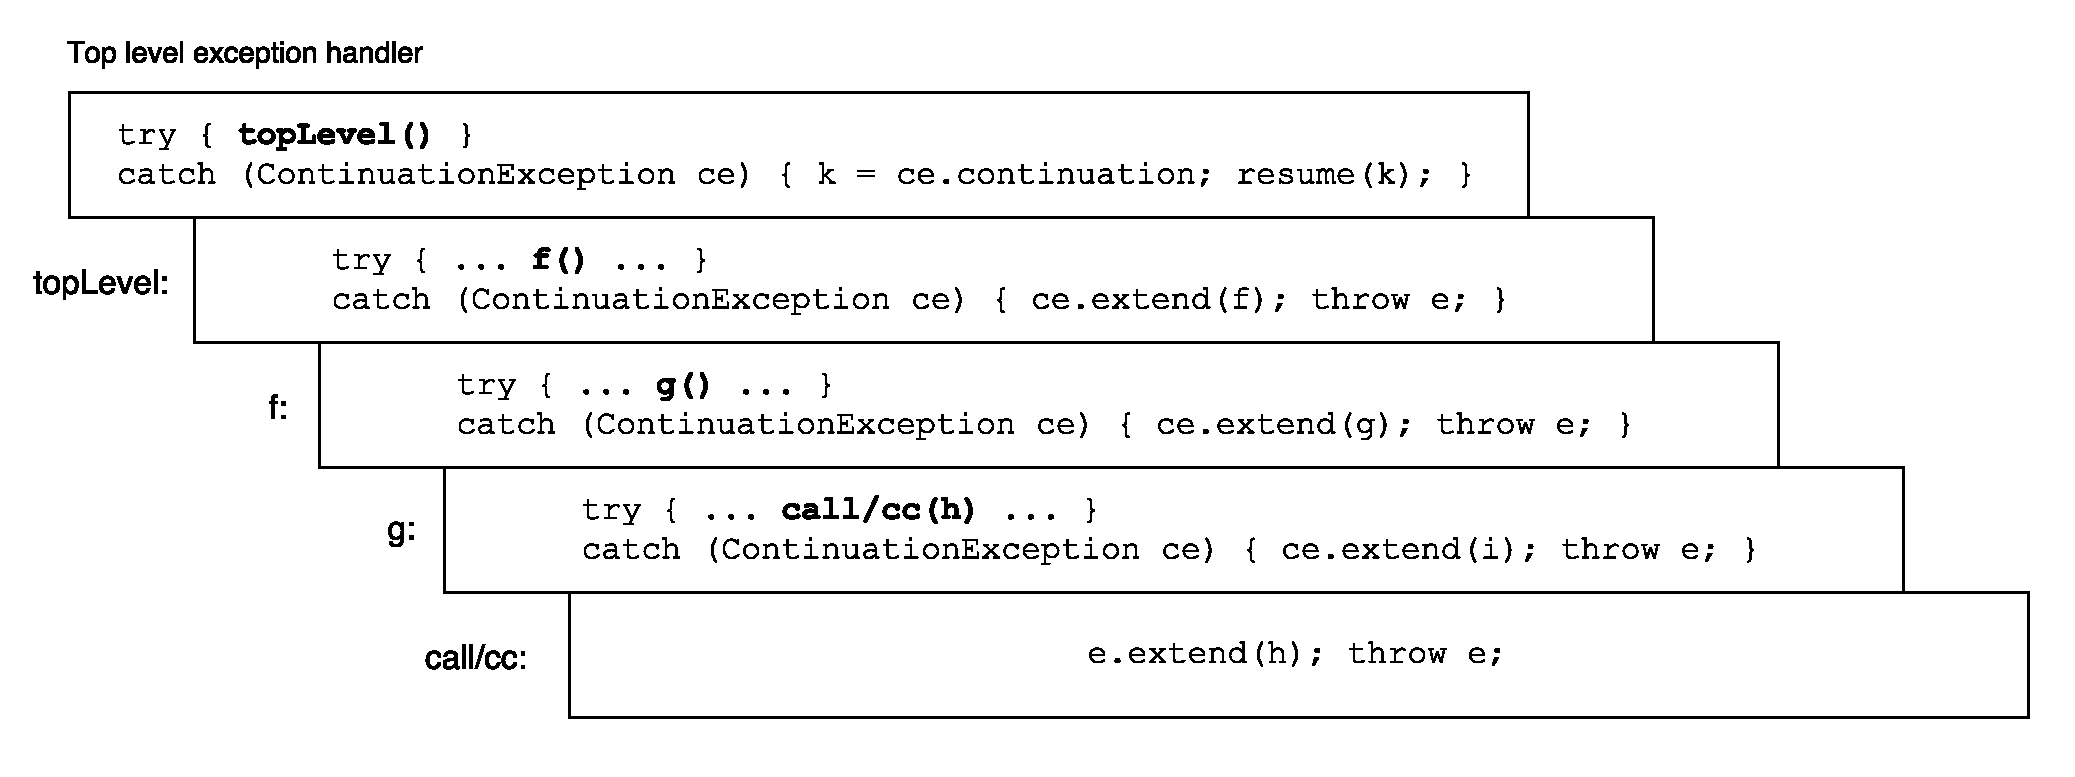
\includegraphics{figures/stack.pdf}
\caption{\label{stack}}
\end{figure}

When the \texttt{call/cc} is called, it creates a new
\texttt{ContinuationException} object, adds the computation associated
to \texttt{h} to the list, and throws the exception. Just after the
\texttt{throw}, the execution stops and the JVM searches routines in the
stack for an exception handler. The first \texttt{try}/\texttt{catch}
expression found, that is in \texttt{g}, extends the list with an other
computation and re-throws the exception.

\begin{figure}[htbp]
\centering
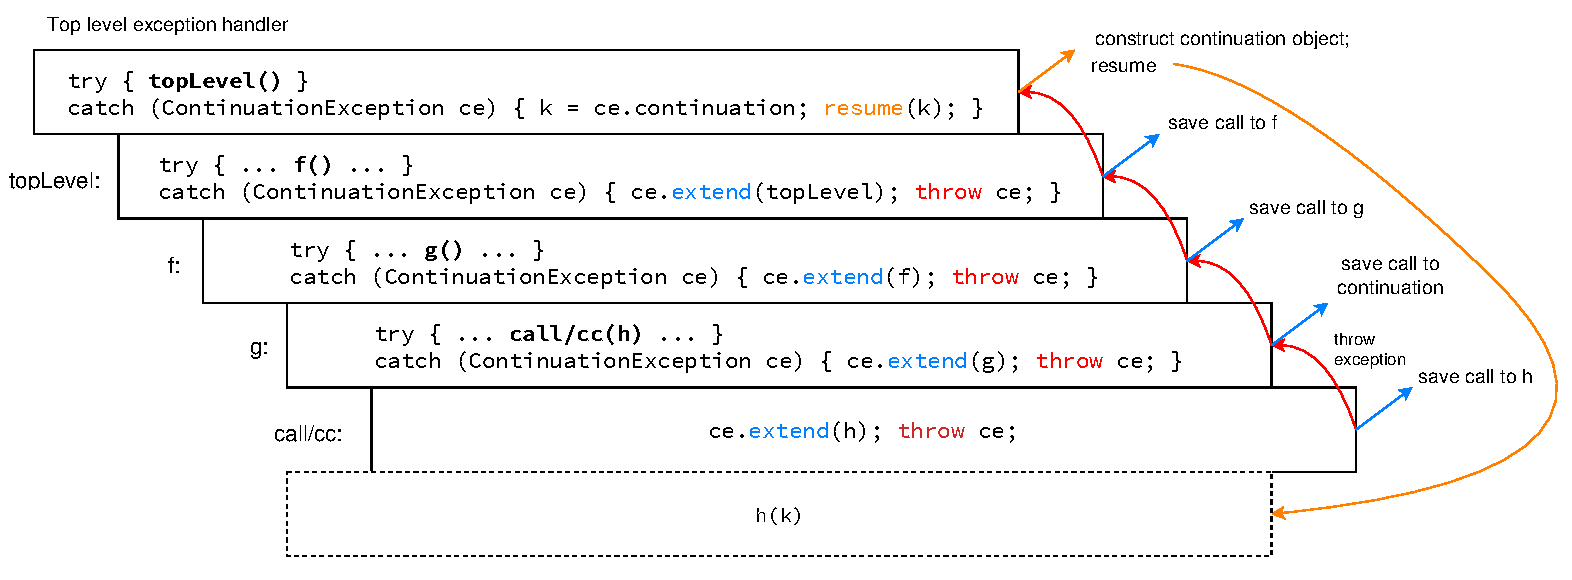
\includegraphics{figures/stack_mod.pdf}
\caption{\label{stack-mod}}
\end{figure}

The exception goes past the try block to try blocks in an outer scope.
At each step a new computation is added to the
\texttt{ContinuationException}, until the control goes to the top level
exception handler, which assembles the actual exception object.
Searching in outer scopes for exception handlers is called a \emph{stack
walk}. While the stack unwinds, the JVM pops the stack frames off of the
stack, destroying all the stack allocated variables. However, as all the
computation steps are saved in the \texttt{ContinuationException}, a
copy of the stack is progressively created on the heap. The exception
always maintains a reference to the list of computations during the
stack walk, so that the continuation is not garbage-collected.

The top level handler, besides assembling the continuation object,
resumes the execution of \texttt{h}, the function passed to the
\texttt{call/cc}, passing to it the continuation as argument. If
\texttt{h} does not invoke the continuation, the top level handler
resumes the continuation after \texttt{h} returns. Figure
\ref{stack-mod} illustrates the process.

\begin{figure}[htbp]
\centering
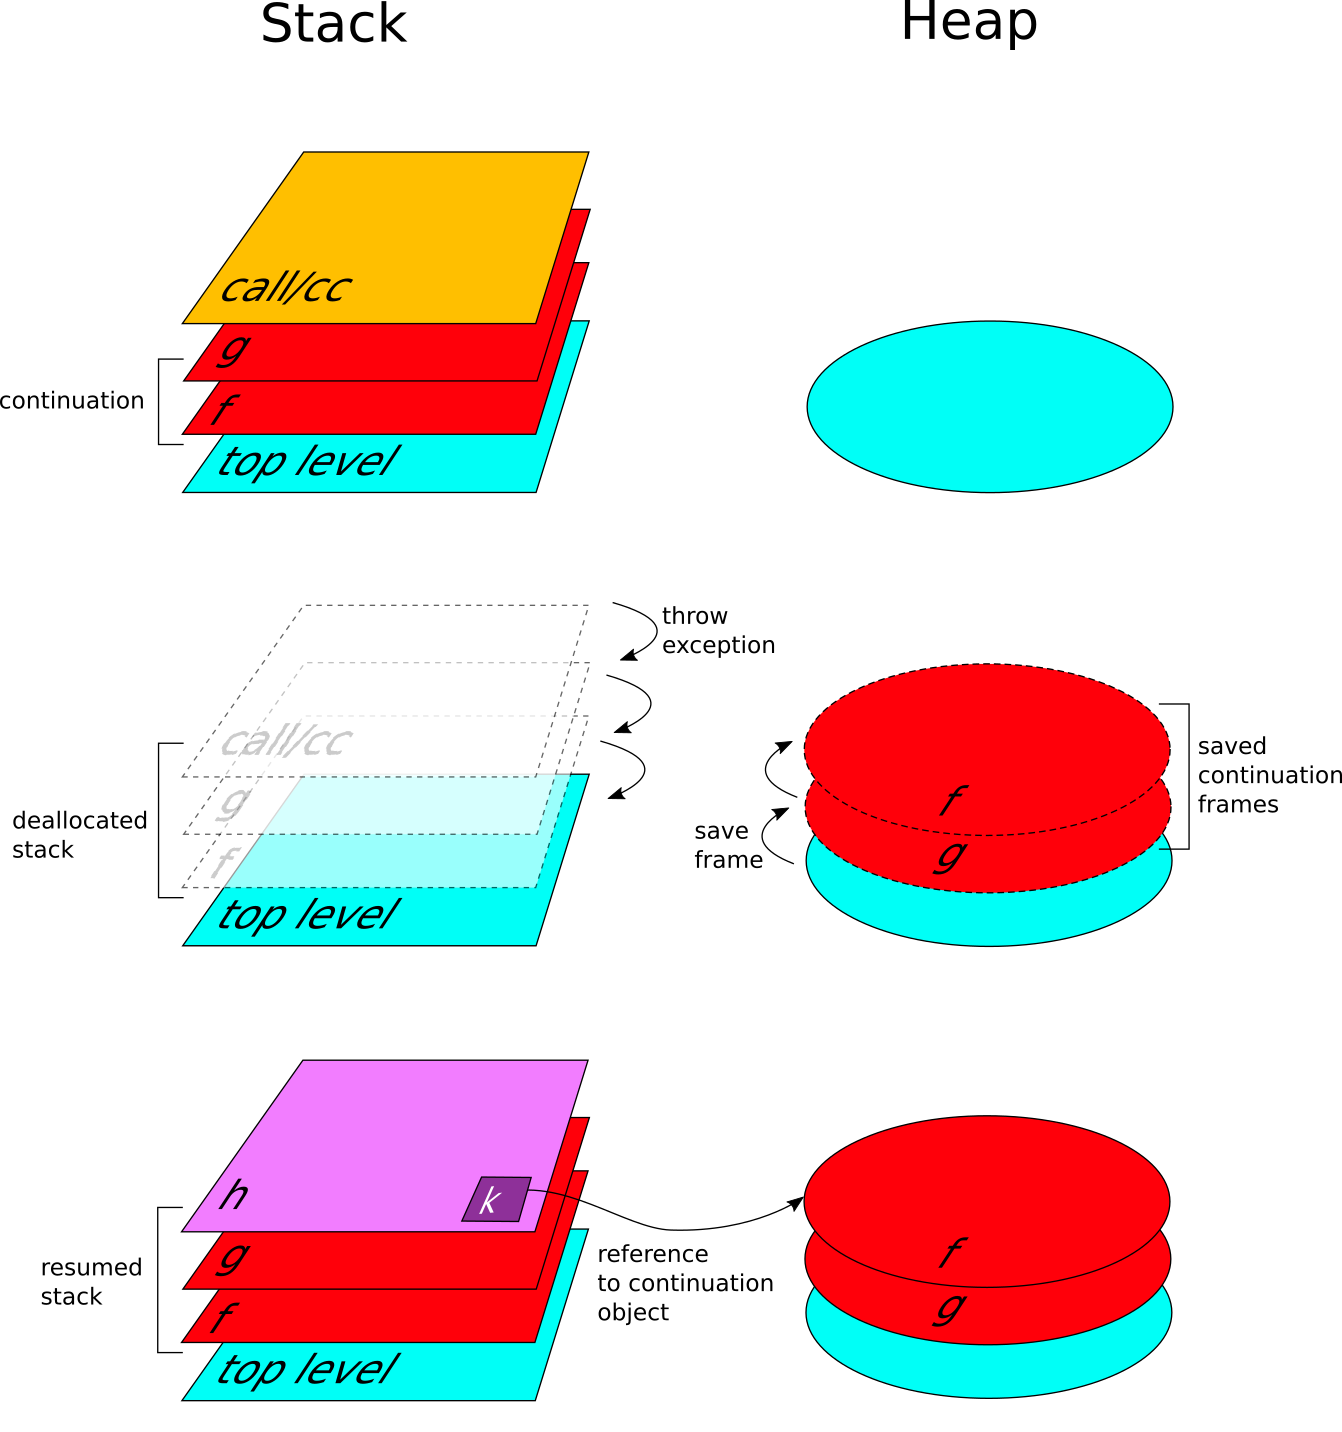
\includegraphics{figures/frames.png}
\caption{Stack and heap during a continuation capture \label{frames}}
\end{figure}

Figure \ref{frames} shows what happens in the stack and in the heap when
a continuation is captured by \texttt{call/cc}. When \texttt{call/cc} is
called the stack frames belonging to the continuation are under the
\texttt{call/cc}'s one (assuming the stack growing bottom-up). Throwing
the \texttt{ContinuationException}, \texttt{call/cc} starts to unwind
the stack, and consequently the heap starts to be populated by the
continuation frames. When top level is reached, the handler creates the
continuation object. At the end of the process, the \texttt{h} function
is resumed with the continuation object bound to its single argument.

\begin{figure}[htbp]
\centering
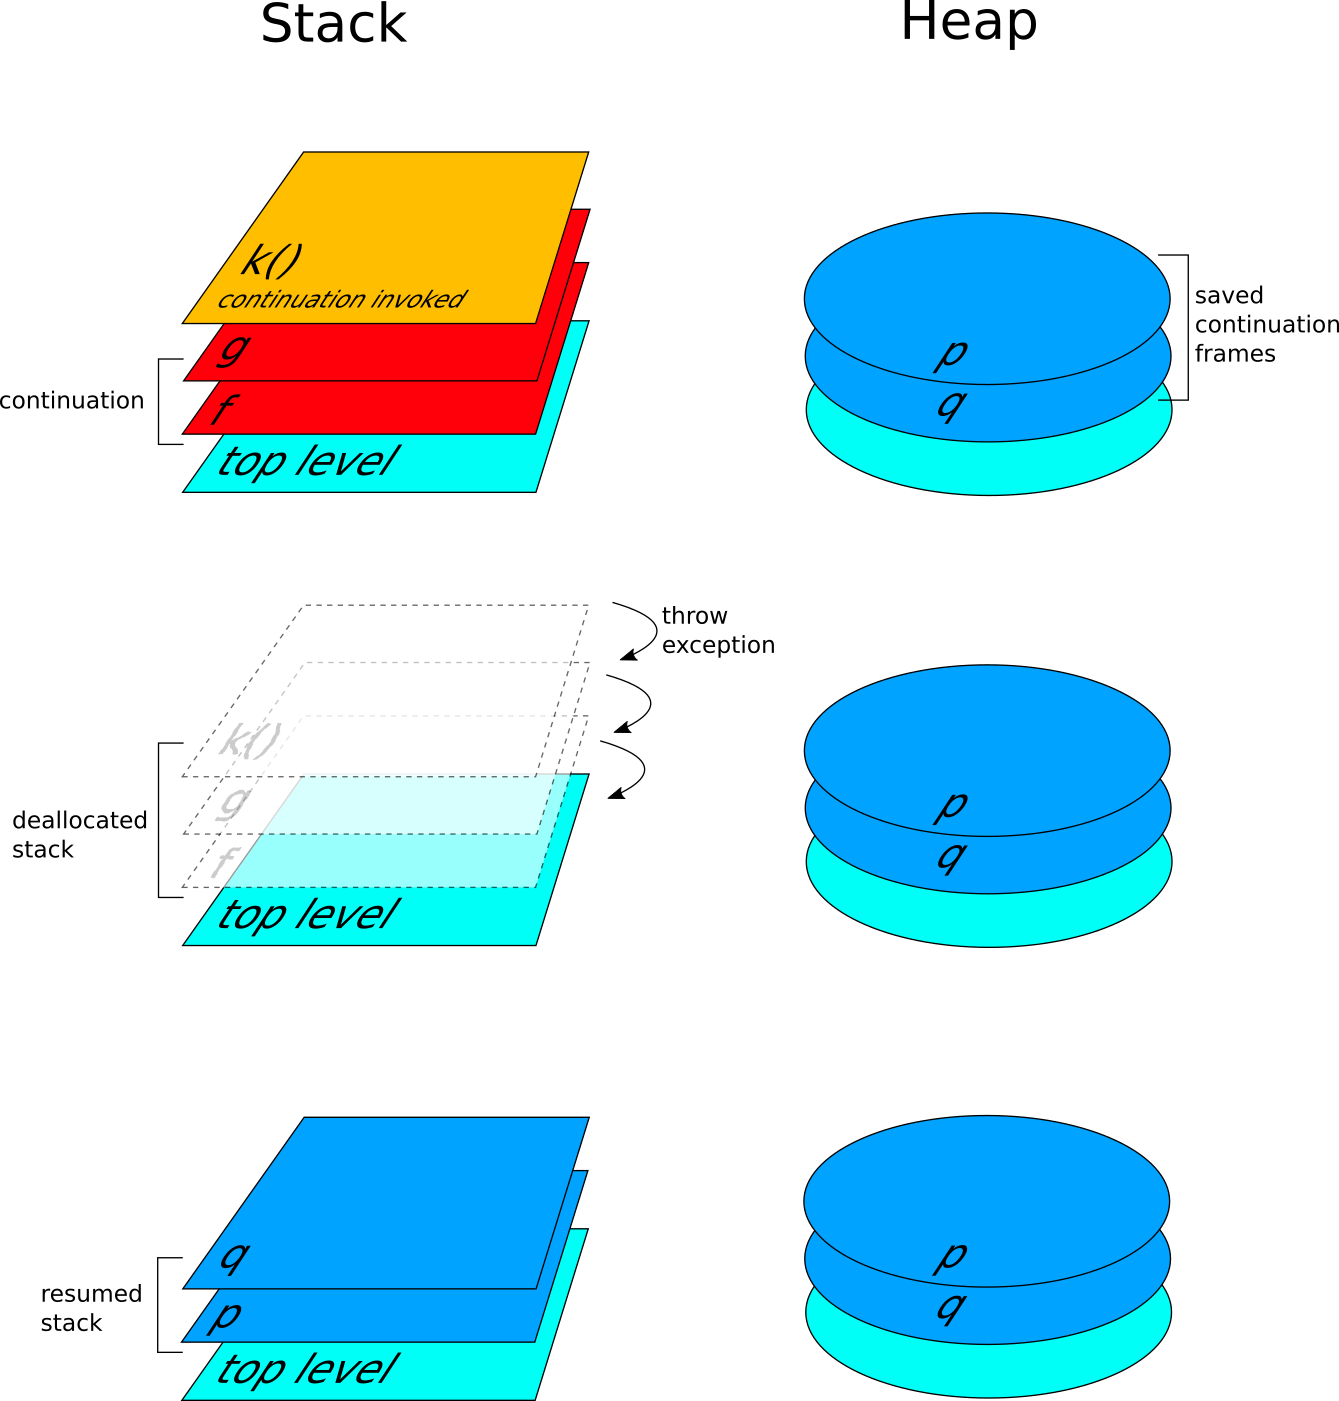
\includegraphics{figures/frames-call.png}
\caption{Stack and heap when reinstating a continuation
\label{frames-call}}
\end{figure}

An interesting property of first-class continuations is that they can be
invoked at any time, provided that they are saved in an accessible
variable. When a continuation is invoked, it throws an
\texttt{ExitException}. This causes the stack to be unwind, as in the
capture case. The top level handler in this case resumes the
continuation frames stored in the continuation object. The final result
is that the execution restart where it was suspended by the call/cc,
while the heap continues to store the continuation object. This can be
accessed other times, or can be garbage-collected if it is no more used.

\section{Generalised stack inspection for a JVM-based
Scheme}\label{generalised-stack-inspection-for-a-jvm-based-scheme}

This section shows how the generalised stack inspection technique
described by Pettyjohn et al. can be adapted to be used on the JVM, and
how it can be included in a Scheme compiler. We will see also how some
issues leaved open by the original paper have been tackled.

\subsection{Assignment conversion}\label{assignment-conversion}

In our case, this step is not necessary. Indeed, management of shared
variable bindings is an orthogonal issue with respect to our global
transformation, and it is shared between all the languages that provide
lexical closures. Kawa already supports lexical closures, so has its way
of managing variable bindings. For each closure, Kawa creates a new
class to represent a function together with the environment of captured
variables.

\subsection{A-Normalization}\label{a-normalization}

The first step of the process is to transform the source to A-normal
form. ANF was introduced by Flanagan et al. in
{[}\hyperref[ref-Flanagan1993]{34}{]} as an intermediate representation
for compilers. It encodes data flow explicitly by naming all
sub-expressions within the program and permitting only a single
definition of any particular variable. The paper by Flanagan et al. also
presents a basic linear-time A-normalization algorithm for a subset of
Scheme. The algorithm can be easily extended to handle top-level defines
and side effects {[}\hyperref[ref-ANFMight2015]{41}{]}. Being Kawa a
super-set of R7RS Scheme and having also many Java related extensions,
the code of the original A-normalizer must be further extended. Instead
of performing the transformation directly on the Scheme source, I opted
for performing it on the abstract syntax tree, as it already uses a
reduced set of expression types.

The following code shows an instance of the transformation in three
steps. The \emph{return} operation corresponds to the identity function,
while the \emph{bind} operation is a function that constructs let
bindings to make every atomic computation explicit (the bind here has
the same purpose as the \texttt{normalizeName} function in the Flanagan
et al. paper).

The syntax tree is traversed starting from the root, and each non-atomic
expression is passed to the \texttt{bind} with another parameter, called
\emph{context} (the very first context is the identity function that
returns its argument). The context is a function that can be invoked.
When the visiting process reaches a non-atomic expression a new context
is created, and the passed context is called only inside the new one.
The \texttt{bind} function has two purposes:

\begin{enumerate}
\def\labelenumi{\arabic{enumi}.}
\tightlist
\item
  to create a context, that generates a \texttt{let} expression to
  let-bind the expression next to come in the traversing process;
\item
  to visit the passed expression, to continue the syntax tree
  traversing.
\end{enumerate}

This chain finish when a leaf (an atomic expression) is encountered in
the tree, in this case the passed context is invoked (which in turn will
invoke the previous context and so on). At this point the chain of
context invocations starts to wrap each expression in a \texttt{let}
binding, processing the expressions backward, and enclosing them step by
step in nested \texttt{let} expressions. This backward traversing stops
when the context called is the identity function. This happens in the
leaves.

When the expression to normalize is a conditional, the \texttt{bind} is
used on each branch expression. Instead of creating a let binding for
each branch, as they cannot be evaluated before the test outcome,
\texttt{bind} calls the visit method with the identity context,
restarting the normalization in each branch.

The following code shows the a-normalization process for a simple Scheme
expression. Note that the internal \texttt{if} expression should be
further normalized, but we consider it atomic here, to keep the example
short. The algoritm performs a monadic transformation combining three
steps:

\begin{enumerate}
\def\labelenumi{\arabic{enumi}.}
\tightlist
\item
  Monadic conversion:
\end{enumerate}

\begin{Shaded}
\begin{Highlighting}[]
   \NormalTok{(}\KeywordTok{+} \DecValTok{1}                             \NormalTok{(bind (}\KeywordTok{if} \NormalTok{(}\KeywordTok{>=} \NormalTok{x }\DecValTok{0}\NormalTok{)}
      \NormalTok{(}\KeywordTok{if} \NormalTok{(}\KeywordTok{>=} \NormalTok{x }\DecValTok{0}\NormalTok{)                            (f x)}
          \NormalTok{(f x)             -->               (return }\DecValTok{0}\NormalTok{))}
          \DecValTok{0}\NormalTok{))                             (}\KeywordTok{lambda} \NormalTok{(t) (}\KeywordTok{+} \DecValTok{1} \NormalTok{t)))}
\end{Highlighting}
\end{Shaded}

\begin{enumerate}
\def\labelenumi{\arabic{enumi}.}
\setcounter{enumi}{1}
\tightlist
\item
  The result is interpreted in the identity monad:
\end{enumerate}

\begin{Shaded}
\begin{Highlighting}[]
                \NormalTok{(return a)  }\KeywordTok{=>}  \NormalTok{a}

   \NormalTok{(bind a (}\KeywordTok{lambda} \NormalTok{(x) b))  }\KeywordTok{=>}  \NormalTok{(}\KeywordTok{let} \NormalTok{((x a)) b)}


   \NormalTok{(bind (}\KeywordTok{if} \NormalTok{(}\KeywordTok{>=} \NormalTok{x }\DecValTok{0}\NormalTok{)               (}\KeywordTok{let} \NormalTok{((t (}\KeywordTok{if} \NormalTok{(}\KeywordTok{>=} \NormalTok{x }\DecValTok{0}\NormalTok{)}
             \NormalTok{(f x)          -->                  (f x)}
             \NormalTok{(return }\DecValTok{0}\NormalTok{))                         (return }\DecValTok{0}\NormalTok{))))}
          \NormalTok{(}\KeywordTok{lambda} \NormalTok{(t) (}\KeywordTok{+} \DecValTok{1} \NormalTok{t)))        (}\KeywordTok{+} \DecValTok{1} \NormalTok{t))}
\end{Highlighting}
\end{Shaded}

\begin{enumerate}
\def\labelenumi{\arabic{enumi}.}
\setcounter{enumi}{2}
\tightlist
\item
  Nested let are flattened:
\end{enumerate}

\begin{Shaded}
\begin{Highlighting}[]
   \NormalTok{(}\KeywordTok{let} \NormalTok{((x (}\KeywordTok{let} \NormalTok{((y a))               (}\KeywordTok{let} \NormalTok{((y a))}
              \NormalTok{b)))          -->          (}\KeywordTok{let} \NormalTok{((x b))}
     \NormalTok{c)                                    c))}
\end{Highlighting}
\end{Shaded}

\subsection{Code fragmentation}\label{code-fragmentation}

This transformation, working on code previously A-normalized, fragments
the code in a sequence of function calls. Each let-bind expression is
enclosed in a lambda closure that accepts one argument. The argument is
an other lambda closure that has in the body the call to the next code
fragment. In this way the original source is rewritten as a sequence of
function calls, each call representing a computation step. This way of
fragmenting the source allows to avoid defining many top level
procedures, that would also require an additional pass to perform live
variable analysis.

An example of the entire transformation is showed below:

\begin{enumerate}
\def\labelenumi{\arabic{enumi}.}
\tightlist
\item
  original source
\end{enumerate}

\begin{Shaded}
\begin{Highlighting}[]
    \NormalTok{(}\KeywordTok{define}\FunctionTok{ incr }\DecValTok{#f}\NormalTok{)}

    \NormalTok{(}\KeywordTok{+} \NormalTok{(}\KeywordTok{call/cc}
          \NormalTok{(}\KeywordTok{lambda} \NormalTok{(k)}
              \NormalTok{(set! incr k)}
              \DecValTok{0}\NormalTok{))}
      \DecValTok{1}\NormalTok{) }\CommentTok{; => 1}
\end{Highlighting}
\end{Shaded}

\begin{enumerate}
\def\labelenumi{\arabic{enumi}.}
\setcounter{enumi}{1}
\tightlist
\item
  after A-normalization
\end{enumerate}

\begin{Shaded}
\begin{Highlighting}[]
    \NormalTok{(}\KeywordTok{let} \NormalTok{((v1 (}\KeywordTok{lambda} \NormalTok{(k)              }\CommentTok{; computation #1}
            \NormalTok{(}\KeywordTok{let} \NormalTok{((v0 (set! incr k)))}
              \DecValTok{0}\NormalTok{))))}
     \NormalTok{(}\KeywordTok{let} \NormalTok{((v2 (}\KeywordTok{call/cc} \NormalTok{v1)))          }\CommentTok{; computation #2}
       \NormalTok{(}\KeywordTok{+} \NormalTok{v2 }\DecValTok{1}\NormalTok{))))                     }\CommentTok{; computation #3}
\end{Highlighting}
\end{Shaded}

\begin{enumerate}
\def\labelenumi{\arabic{enumi}.}
\setcounter{enumi}{2}
\tightlist
\item
  after fragmentation
\end{enumerate}

\begin{Shaded}
\begin{Highlighting}[]
    \NormalTok{((}\KeywordTok{lambda} \NormalTok{(incr_an1)                }\CommentTok{; fragment #1}
      \NormalTok{(}\KeywordTok{let} \NormalTok{((v1 (}\KeywordTok{lambda} \NormalTok{(k)}
                  \NormalTok{(}\KeywordTok{let} \NormalTok{((v0 (set! incr k)))}
                    \DecValTok{0}\NormalTok{))))}
         \NormalTok{(incr_an1 v1)))}
     \NormalTok{(}\KeywordTok{lambda} \NormalTok{(v1)}
       \NormalTok{((}\KeywordTok{lambda} \NormalTok{(incr_an2)             }\CommentTok{; fragment #2}
          \NormalTok{(}\KeywordTok{let} \NormalTok{((v2 (}\KeywordTok{call/cc} \NormalTok{v1)))}
            \NormalTok{(incr_an2 v2)))}
        \NormalTok{(}\KeywordTok{lambda} \NormalTok{(v2)}
          \NormalTok{(}\KeywordTok{+} \NormalTok{v2 }\DecValTok{1}\NormalTok{)))))                 }\CommentTok{; fragment #3}
\end{Highlighting}
\end{Shaded}

\subsection{Live variable analysis and closure
conversion}\label{live-variable-analysis-and-closure-conversion}

Kawa's support for lexical closures allows to completely avoid these
steps. Each fragment, created as described in the previous section, is
closed over the values of the variables that are live at that point.

A continuation will be composed of a series of frames. A \emph{frame} is
an object with a method that accepts a single value (the argument to the
continuation) and invokes the appropriate procedure fragment, to
continue the computation from the capture point. Also these frames will
be closed over the next fragment to call.

\subsection{Code Instrumentation}\label{code-instrumentation}

Beside fragmentation, instrumentation is performed for installing
exception handlers around each computation step to enable the capture
and resume of continuations. Kawa supports \texttt{try-catch}
expressions, which are translated directly to native \texttt{try/catch}
statements in Java bytecode. A \texttt{try-catch} expression is created
around each computation to capture a possible
\texttt{ContinuationException}. The installed exception handler adds a
new frame (an invokable object enclosing a call the next computation
step) to the list of frames included inside the
\texttt{ContinuationException} object, then rethrows the exception.

The following code resembles the final result after instrumentation:

\begin{Shaded}
\begin{Highlighting}[]
    \NormalTok{((}\KeywordTok{lambda} \NormalTok{(incr_an1)}
      \NormalTok{(}\KeywordTok{let} \NormalTok{((v1 (}\KeywordTok{lambda} \NormalTok{(k)}
                  \NormalTok{(}\KeywordTok{let} \NormalTok{((v0 (set! incr k)))}
                    \DecValTok{0}\NormalTok{))))}
         \NormalTok{(incr_an1 v1)))}
     \NormalTok{(}\KeywordTok{lambda} \NormalTok{(v1)}
       \NormalTok{((}\KeywordTok{lambda} \NormalTok{(incr_an2)}
          \NormalTok{(}\KeywordTok{let} \NormalTok{((v2 (try-catch (}\KeywordTok{call/cc} \NormalTok{v1)             }\CommentTok{; try/catch}
                      \NormalTok{(cex <ContinuationException>      }\CommentTok{; handler}
                         \NormalTok{(}\KeywordTok{let} \NormalTok{((f (}\KeywordTok{lambda} \NormalTok{(continue-value)}
                                    \NormalTok{(incr_an2 continue-value))))}
                         \NormalTok{(cex:extend (<ContinuationFrame> f))}
                         \NormalTok{(throw cex))))))               }\CommentTok{; re-throw}
            \NormalTok{(incr_an2 v2)))}
        \NormalTok{(}\KeywordTok{lambda} \NormalTok{(v2)}
          \NormalTok{(}\KeywordTok{+} \NormalTok{v2 }\DecValTok{1}\NormalTok{)))))}
\end{Highlighting}
\end{Shaded}

\section{Issues}\label{issues}

\subsection{\texorpdfstring{\texttt{call/cc} in higher order
functions}{call/cc in higher order functions}}\label{callcc-in-higher-order-functions}

Since Kawa optimise some built-in procedures (like \texttt{map},
\texttt{foreach} and \texttt{filter}) implementing them as Java methods,
and because of the global transformation needed by the \texttt{call/cc},
continuations cannot be captured inside functions passed to those higher
order functions. Indeed, the Java implementation of map
(\texttt{gnu.kawa.functions.Map}) is not `aware' of continuations, thus
when you use \texttt{call/cc} inside the lambda passed to \texttt{map},
it will not be able to handle a \texttt{ContinuationException},
resulting in a runtime error.

In the next chapter, we will see a possible solution to this problem.

\subsection{Code size}\label{code-size}

The creation of fragments will introduce a number of extra code.
Although the overhead should be small, there will be an increase in code
size proportional to the number of code fragments.

Code instrumentation introduces a number of \texttt{try/catch} blocks.
This will also increase code size proportional to the number of code
fragments. Chapter 6 will present an estimate of the code size increase.

\subsection{Integration}\label{integration}

Given that the code transformation needed to support continuations adds
a overhead to the compilation process and the generated bytecode, it is
necessary to implement A-normalization and instrumentation as optional
passes, that can be enabled only when we want to use \texttt{call/cc}.
This adds the challenge of integrating such a global transformation in
Kawa, avoiding to make too many changes to the compiler.

\chapter{A call/cc implementation for
Kawa}\label{a-callcc-implementation-for-kawa}

\begin{quote}
\emph{``Do\ldots{} or do not. There is no try.''}

\begin{flushright}
The Empire Strikes Back (film, 1980)
\end{flushright}
\end{quote}

\section{An instance of the transformation in
Java}\label{an-instance-of-the-transformation-in-java}

As a first preliminary step, I ported the C\# code in
{[}\hyperref[ref-StackHack2005]{32}{]} to Java, to study the feasibility
of the technique on the JVM. The code represents a single instance of
the transformation for a simple fibonacci function, and implements some
support functions and data structures. Given that the global
transformation fragments the original source in many function calls, I
produced four versions of the transformed code, to compare the
performance of different type of calls on the JVM:

\begin{enumerate}
\def\labelenumi{\arabic{enumi}.}
\tightlist
\item
  The first one uses nested static classes to implement the continuation
  frames of the function to be run:
\end{enumerate}

\begin{Shaded}
\begin{Highlighting}[]
    \KeywordTok{class} \NormalTok{fib_frame0 }\KeywordTok{extends} \NormalTok{Frame \{}

        \DataTypeTok{int} \NormalTok{x;}

        \KeywordTok{public} \FunctionTok{fib_frame0}\NormalTok{(}\DataTypeTok{int} \NormalTok{x) \{ }\KeywordTok{this}\NormalTok{.}\FunctionTok{x} \NormalTok{= x; \}}
        \FunctionTok{@Override}
        \KeywordTok{public} \NormalTok{Object }\FunctionTok{invoke}\NormalTok{(Object return_value)}
                \KeywordTok{throws} \NormalTok{ContinuationException, Throwable \{}
            \CommentTok{// call to the next fragment}
            \KeywordTok{return} \FunctionTok{fib_an0}\NormalTok{(x);}
        \NormalTok{\}}
    \NormalTok{\}}

    \KeywordTok{public} \DataTypeTok{int} \FunctionTok{fib_an}\NormalTok{(}\DataTypeTok{int} \NormalTok{x)}
          \KeywordTok{throws} \NormalTok{ContinuationException, Throwable \{}
        \KeywordTok{try} \NormalTok{\{}
            \FunctionTok{pause}\NormalTok{();}
        \NormalTok{\} }\KeywordTok{catch} \NormalTok{(ContinuationException sce) \{}
            \NormalTok{sce.}\FunctionTok{extend}\NormalTok{(}\KeywordTok{new} \FunctionTok{ContinuationFrame}\NormalTok{(}\KeywordTok{new} \FunctionTok{fib_frame0}\NormalTok{(x)));}
            \KeywordTok{throw} \NormalTok{sce;}
        \NormalTok{\}}

        \KeywordTok{return} \FunctionTok{fib_an0}\NormalTok{(x);}
    \NormalTok{\}}
\end{Highlighting}
\end{Shaded}

\begin{enumerate}
\def\labelenumi{\arabic{enumi}.}
\setcounter{enumi}{1}
\tightlist
\item
  the second version uses \texttt{MethodHandle}s, that were introduced
  in Java 7. A \texttt{MethodHandle} is a typed, directly executable
  reference to an underlying method, constructor or field:
\end{enumerate}

\begin{Shaded}
\begin{Highlighting}[]
    \DataTypeTok{static} \NormalTok{Object }\FunctionTok{fib_frame0_invoke}\NormalTok{(Object x, Object continue_value)}
            \KeywordTok{throws} \NormalTok{SaveContinuationException, Exception \{}
         \KeywordTok{return} \FunctionTok{fib_an0} \NormalTok{((}\DataTypeTok{int}\NormalTok{) x);}
    \NormalTok{\}}

    \DataTypeTok{static} \NormalTok{MethodHandle }\FunctionTok{fib_frame0}\NormalTok{(}\DataTypeTok{int} \NormalTok{x)}
            \KeywordTok{throws} \NormalTok{Exception \{}
        \NormalTok{MethodType mt = MethodType.}\FunctionTok{methodType}\NormalTok{(Object.}\FunctionTok{class}\NormalTok{,}
                                              \NormalTok{Object.}\FunctionTok{class}\NormalTok{,}
                                              \NormalTok{Object.}\FunctionTok{class}\NormalTok{);}
        \NormalTok{MethodHandle handle = lookup.}\FunctionTok{findStatic}\NormalTok{(fib_mh.}\FunctionTok{class}\NormalTok{,}
                                                \StringTok{"fib_frame0_invoke"}\NormalTok{,}
                                                \NormalTok{mt);}

        \KeywordTok{return} \NormalTok{handle.}\FunctionTok{bindTo}\NormalTok{(x);}
    \NormalTok{\}}

    \KeywordTok{public} \DataTypeTok{static} \DataTypeTok{int} \FunctionTok{fib_an}\NormalTok{(}\DataTypeTok{int} \NormalTok{x)}
           \KeywordTok{throws} \NormalTok{SaveContinuationException, Exception \{}
        \KeywordTok{try} \NormalTok{\{}
            \FunctionTok{pause}\NormalTok{();}
        \NormalTok{\} }\KeywordTok{catch} \NormalTok{(SaveContinuationException sce) \{}
            \NormalTok{sce.}\FunctionTok{Extend}\NormalTok{(}\KeywordTok{new} \FunctionTok{ContinuationFrame}\NormalTok{(}\FunctionTok{fib_frame0}\NormalTok{(x)));}
            \KeywordTok{throw} \NormalTok{sce;}
        \NormalTok{\}}

        \KeywordTok{return} \FunctionTok{fib_an0}\NormalTok{(x);}
    \NormalTok{\}}
\end{Highlighting}
\end{Shaded}

\begin{enumerate}
\def\labelenumi{\arabic{enumi}.}
\setcounter{enumi}{2}
\tightlist
\item
  the third version uses Java 8 lambdas, specified with the new Java
  syntax:
\end{enumerate}

\begin{Shaded}
\begin{Highlighting}[]
    \DataTypeTok{static} \NormalTok{Object }\FunctionTok{fib_frame0_invoke}\NormalTok{(Object x, Object continue_value)}
            \KeywordTok{throws} \NormalTok{SaveContinuationException, Exception \{}
         \KeywordTok{return} \FunctionTok{fib_an0} \NormalTok{((}\DataTypeTok{int}\NormalTok{) x);}
    \NormalTok{\}}

    \DataTypeTok{static} \NormalTok{Frame }\FunctionTok{fib_frame0}\NormalTok{(}\DataTypeTok{int} \NormalTok{x)}
            \KeywordTok{throws} \NormalTok{Exception \{}
        \NormalTok{Frame f = (Object continue_value)}
                   \NormalTok{-> \{}
                        \KeywordTok{return} \FunctionTok{fib_frame0_invoke}\NormalTok{(x, continue_value);}
                      \NormalTok{\};}
        \KeywordTok{return} \NormalTok{f;}
    \NormalTok{\}}

    \KeywordTok{public} \DataTypeTok{static} \DataTypeTok{int} \FunctionTok{fib_an}\NormalTok{(}\DataTypeTok{int} \NormalTok{x)}
            \KeywordTok{throws} \NormalTok{SaveContinuationException, Exception \{}
        \KeywordTok{try} \NormalTok{\{}
            \FunctionTok{pause}\NormalTok{();}
        \NormalTok{\} }\KeywordTok{catch} \NormalTok{(SaveContinuationException sce) \{}
            \NormalTok{sce.}\FunctionTok{Extend}\NormalTok{(}\KeywordTok{new} \FunctionTok{ContinuationFrame}\NormalTok{(}\FunctionTok{fib_frame0}\NormalTok{(x)));}
            \KeywordTok{throw} \NormalTok{sce;}
        \NormalTok{\}}

        \KeywordTok{return} \FunctionTok{fib_an0}\NormalTok{(x);}
    \NormalTok{\}}
\end{Highlighting}
\end{Shaded}

\begin{enumerate}
\def\labelenumi{\arabic{enumi}.}
\setcounter{enumi}{3}
\tightlist
\item
  the last version generates lambdas explicitly using LambdaMetafactory,
  an API introduced in Java 8 to facilitate the creation of simple
  function objects.
\end{enumerate}

\begin{Shaded}
\begin{Highlighting}[]
    \NormalTok{fib_frame0_factory}
        \NormalTok{= LambdaMetafactory}
            \NormalTok{.}\FunctionTok{metafactory}\NormalTok{(lookup,}
                         \StringTok{"invoke"}\NormalTok{,}
                         \NormalTok{invokedType,}
                         \NormalTok{methodType,}
                         \NormalTok{lookup.}\FunctionTok{findStatic}\NormalTok{(fib_meta.}\FunctionTok{class}\NormalTok{,}
                                           \StringTok{"fib_frame0_invoke"}\NormalTok{,}
                                           \NormalTok{implType),}
                         \NormalTok{methodType).}\FunctionTok{dynamicInvoker}\NormalTok{();}

    \DataTypeTok{static} \NormalTok{Object }\FunctionTok{fib_frame0_invoke}\NormalTok{(Object x, Object continue_value)}
            \KeywordTok{throws} \NormalTok{SaveContinuationException, Throwable \{}
         \KeywordTok{return} \FunctionTok{fib_an0} \NormalTok{((}\DataTypeTok{int}\NormalTok{) x);}
    \NormalTok{\}}

    \DataTypeTok{static} \NormalTok{Frame }\FunctionTok{fib_frame0}\NormalTok{(}\DataTypeTok{int} \NormalTok{x)}
            \KeywordTok{throws} \NormalTok{Throwable \{}
        \KeywordTok{return} \NormalTok{(Frame) fib_frame0_factory.}\FunctionTok{invoke}\NormalTok{(x);}
    \NormalTok{\}}
\end{Highlighting}
\end{Shaded}

I tested each type of method call with JMH
{[}\hyperref[ref-jmh2015]{42},
\hyperref[ref-BenchmarkingJVM2015]{43}{]}, a benchmarking framework for
the JVM. Figures \ref{calls-table} , \ref{calls} show the results. The
lambda case is quite fast, if compared with MethodHandles, but also the
explicit use of LambdaMetafactory gives good results, provided that the
call to LambdaMetafactory.metafactory is cached in a static field.
However, the difference in performance between lambda calls and regular
method calls is negligible. Thus is not worth to re-design a significant
part of the compiler, and to loose the compatibility with previous
version of the JVM, for such a small improvement.

\begin{figure}[htbp]
\centering
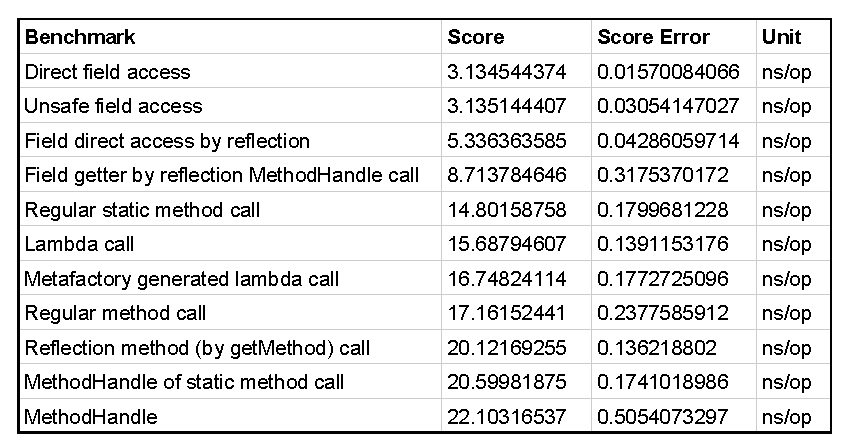
\includegraphics{figures/calls-table.pdf}
\caption{Performance comparison of different types of call in Java
\label{calls-table}}
\end{figure}

\begin{figure}[htbp]
\centering
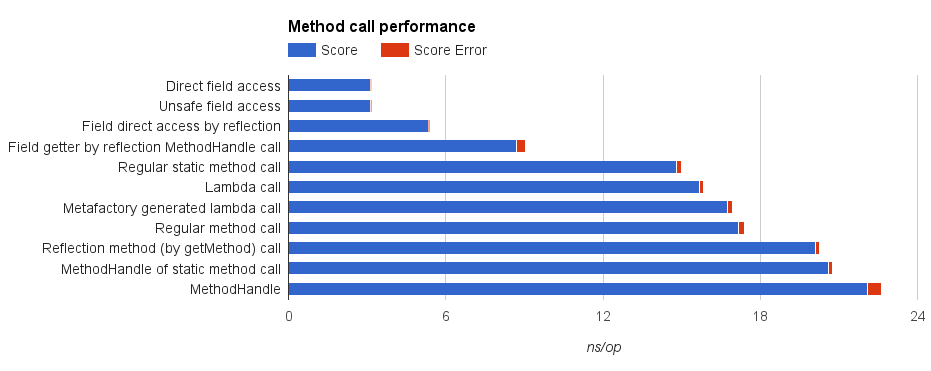
\includegraphics{figures/calls.png}
\caption{Performance comparison of different types of call in Java
\label{calls}}
\end{figure}

\subsection{Exceptions performance in
Java}\label{exceptions-performance-in-java}

The capture of a continuation, and in particular the stack copying
mechanism, is driven by exception throwing and exception handling.
Therefore, is crucial to understand how the installation of exception
handlers and the construction of an Exception object impact the
performance.

In Java, when throwing an exception, the most expensive operation is the
construction of the stack trace, that is useful for debugging reasons.
As well as we are not using exceptions with they original purpose, we
can have rid of the stack trace construction and optimise the
\texttt{Exception} object. It is sufficient to override the
\texttt{fillInStackTrace} method of \texttt{Throwable}:

\begin{Shaded}
\begin{Highlighting}[]
    \KeywordTok{public} \DataTypeTok{static} \KeywordTok{class} \NormalTok{FastException }\KeywordTok{extends} \NormalTok{Exception \{}

        \FunctionTok{@Override}
        \KeywordTok{public} \NormalTok{Throwable }\FunctionTok{fillInStackTrace}\NormalTok{() \{}
            \KeywordTok{return} \KeywordTok{this}\NormalTok{;}
        \NormalTok{\}}
    \NormalTok{\}}
\end{Highlighting}
\end{Shaded}

I performed a straightforward benchmark, comparing the time spent by a
regular method call, a method call surrounded by an exception handler, a
method call throwing a caught exception and a method call throwing a
\texttt{FastException}.

\begin{Shaded}
\begin{Highlighting}[]
        \CommentTok{// case 1}
        \NormalTok{t.}\FunctionTok{method1}\NormalTok{(i);}

        \CommentTok{// case 2}
        \KeywordTok{try} \NormalTok{\{}
            \NormalTok{t.}\FunctionTok{method2}\NormalTok{(i);}
        \NormalTok{\} }\KeywordTok{catch} \NormalTok{(Exception e) \{}
            \CommentTok{// We will *never* get here}
        \NormalTok{\}}

        \CommentTok{// case 3}
        \KeywordTok{try} \NormalTok{\{}
            \NormalTok{t.}\FunctionTok{method3}\NormalTok{(i);}
        \NormalTok{\} }\KeywordTok{catch} \NormalTok{(Exception e) \{}
            \CommentTok{// We will get here}
        \NormalTok{\}}

        \CommentTok{// case 4}
        \KeywordTok{try} \NormalTok{\{}
            \NormalTok{t.}\FunctionTok{method4}\NormalTok{(i);}
        \NormalTok{\} }\KeywordTok{catch} \NormalTok{(FastException e) \{}
            \CommentTok{// We will get here}
        \NormalTok{\}}
\end{Highlighting}
\end{Shaded}

The results from 10 million iterations are shown in the following table.

\begin{longtable}[c]{@{}ll@{}}
\toprule
& time (ms)\tabularnewline
\midrule
\endhead
regular & 1225\tabularnewline
no caught exception & 1240\tabularnewline
caught exception & 35482\tabularnewline
caught, optimised & 1330\tabularnewline
\bottomrule
\end{longtable}

As you can see, to catch a \texttt{FastException} introduces a
negligible overhead, while instantiating an \texttt{Exception} with its
stack trace is more than an order of magnitude more expensive.

\section{Support code}\label{support-code}

For capturing and resuming continuations we need a framework to support
all the required operations, such as construct an object that models the
continuation, and turn a continuation object back into an actual
continuation.

\begin{Shaded}
\begin{Highlighting}[]
    \KeywordTok{public} \DataTypeTok{static} \KeywordTok{class} \NormalTok{ContinuationFrame \{}

        \NormalTok{Procedure computation;}
        \NormalTok{ArrayList<ContinuationFrame> continuation;}

        \KeywordTok{public} \FunctionTok{ContinuationFrame}\NormalTok{(Procedure frame) \{}
            \NormalTok{computation = frame;}
        \NormalTok{\}}
    \NormalTok{\}}
\end{Highlighting}
\end{Shaded}

The basic blocks of a continuation are its \texttt{ContinuationFrame}s.
A \texttt{ContinuationFr-} \texttt{ame} (for brevity, a frame) is a
simple data structure which contains a single computation (a
\texttt{Procedure} that takes one argument), and a list of
\texttt{ContinuationFrame}s. The list is used by the next capture of a
continuation. All the frames needed to assemble a continuation are
collected using a \texttt{ContinuationException}. This class extends
\texttt{FastException} and stores the list of frames which is extended
step by step by the chain of throws. It contains also a list of frames
that have been already reloaded by a previously call to
\texttt{call/cc}. When the exception reaches the top level exception
handler, this calls the method \texttt{toContinuation} that builds a new
\texttt{Continuation} object using the two lists.

\begin{Shaded}
\begin{Highlighting}[]
\KeywordTok{public} \DataTypeTok{static} \KeywordTok{class} \NormalTok{ContinuationException }\KeywordTok{extends} \NormalTok{FastException \{}

    \NormalTok{ArrayList<ContinuationFrame>}
    \NormalTok{newCapturedFrames = }\KeywordTok{new} \NormalTok{ArrayList<ContinuationFrame>();}

    \NormalTok{ArrayList<ContinuationFrame> reloadedFrames;}

    \KeywordTok{public} \DataTypeTok{void} \FunctionTok{extend}\NormalTok{(ContinuationFrame extension) \{}
        \NormalTok{newCapturedFrames.}\FunctionTok{add}\NormalTok{(extension);}
    \NormalTok{\}}

    \KeywordTok{public} \DataTypeTok{void} \FunctionTok{append}\NormalTok{(ArrayList<ContinuationFrame> oldFrames) \{}
        \NormalTok{reloadedFrames = oldFrames;}
    \NormalTok{\}}

    \KeywordTok{public} \NormalTok{Continuation }\FunctionTok{toContinuation}\NormalTok{() }\KeywordTok{throws} \NormalTok{Exception \{}
        \KeywordTok{return} \KeywordTok{new} \FunctionTok{Continuation}\NormalTok{(newCapturedFrames,}
                                \NormalTok{reloadedFrames);}
    \NormalTok{\}}
\NormalTok{\}}
\end{Highlighting}
\end{Shaded}

The \texttt{Continuation} constructor takes the two lists and assembles
the continuation.

\begin{Shaded}
\begin{Highlighting}[]
\KeywordTok{public} \KeywordTok{class} \NormalTok{Continuation }\KeywordTok{extends} \NormalTok{Procedure0or1 \{}

    \NormalTok{ArrayList<ContinuationFrame> frames;}

    \KeywordTok{public} \FunctionTok{Continuation}\NormalTok{(ArrayList<ContinuationFrame> newFrames,}
                        \NormalTok{ArrayList<ContinuationFrame> oldFrames) \{}

        \NormalTok{frames = (oldFrames != }\KeywordTok{null}\NormalTok{)}
                 \NormalTok{? }\KeywordTok{new} \NormalTok{ArrayList<ContinuationFrame>(oldFrames)}
                 \NormalTok{: }\KeywordTok{new} \NormalTok{ArrayList<ContinuationFrame>();}

        \KeywordTok{for}\NormalTok{(}\DataTypeTok{int} \NormalTok{i = newFrames.}\FunctionTok{size}\NormalTok{()-}\DecValTok{1}\NormalTok{; i >= }\DecValTok{0}\NormalTok{; i--) \{}
            \NormalTok{ContinuationFrame newFrame = newFrames.}\FunctionTok{get}\NormalTok{(i);}
            \KeywordTok{if} \NormalTok{(newFrame.}\FunctionTok{continuation} \NormalTok{!= }\KeywordTok{null}\NormalTok{) \{}
               \KeywordTok{throw} \KeywordTok{new} \NormalTok{Error(}\StringTok{"Continuation should be empty here"}\NormalTok{);}
            \NormalTok{\}}
            \NormalTok{newFrame.}\FunctionTok{continuation}
               \NormalTok{= }\KeywordTok{new} \NormalTok{ArrayList<ContinuationFrame>(frames);}
            \NormalTok{frames.}\FunctionTok{add}\NormalTok{(newFrame);}
        \NormalTok{\}}
    \NormalTok{\}}
\end{Highlighting}
\end{Shaded}

When a continuation is invoked, we actually call the \texttt{apply}
method of \texttt{Continuation}. Here we create a new procedure which,
when called, resumes the continuation. We wrap the procedure in an
exception so that, throwing it, we unload the \emph{current}
continuation. The top level handler will receive this exception and will
use it to resume the \emph{invoked} continuation.

\begin{Shaded}
\begin{Highlighting}[]
    \KeywordTok{public} \NormalTok{Object }\FunctionTok{apply0}\NormalTok{() }\KeywordTok{throws} \NormalTok{Throwable \{}
        \KeywordTok{return} \FunctionTok{apply1}\NormalTok{(Values.}\FunctionTok{empty}\NormalTok{);}
    \NormalTok{\}}

    \KeywordTok{public} \NormalTok{Object }\FunctionTok{apply1}\NormalTok{(}\DataTypeTok{final} \NormalTok{Object val) }\KeywordTok{throws} \NormalTok{Throwable \{}

        \NormalTok{Procedure t = }\KeywordTok{new} \FunctionTok{Procedure1}\NormalTok{() \{}

            \KeywordTok{public} \NormalTok{Object }\FunctionTok{apply1}\NormalTok{(Object ignored) }\KeywordTok{throws} \NormalTok{Throwable \{}
                \KeywordTok{return} \FunctionTok{reloadFrames}\NormalTok{(frames.}\FunctionTok{size}\NormalTok{()-}\DecValTok{2}\NormalTok{, val);}
            \NormalTok{\}}
        \NormalTok{\};}

        \KeywordTok{throw} \KeywordTok{new} \FunctionTok{ExitException}\NormalTok{(t);}
    \NormalTok{\}}
\end{Highlighting}
\end{Shaded}

The \texttt{Continuation} object also contains the method to resume the
continuation. \texttt{reloadFrames} iterates over the list of frames in
reverse order to re-establish the saved continuation reconstructing the
stack. The topmost frame gets the restart value passed into it.

\begin{Shaded}
\begin{Highlighting}[]
    \NormalTok{Object }\FunctionTok{resume}\NormalTok{(}\DataTypeTok{final} \NormalTok{Object restartValue) }\KeywordTok{throws} \NormalTok{Throwable \{}
        \KeywordTok{return} \FunctionTok{reloadFrames}\NormalTok{(frames.}\FunctionTok{size}\NormalTok{()-}\DecValTok{1}\NormalTok{, restartValue);}
    \NormalTok{\}}

    \NormalTok{Object }\FunctionTok{reloadFrames}\NormalTok{(}\DataTypeTok{int} \NormalTok{endIndex, Object restartValue)}
    \KeywordTok{throws} \NormalTok{Throwable \{}
        \NormalTok{Object continueValue = restartValue;}
        \KeywordTok{for} \NormalTok{(}\DataTypeTok{int} \NormalTok{i = endIndex; i >= }\DecValTok{0}\NormalTok{; i -= }\DecValTok{1}\NormalTok{) \{}
            \NormalTok{ContinuationFrame frame = frames.}\FunctionTok{get}\NormalTok{(i);}
            \KeywordTok{try} \NormalTok{\{}
                \NormalTok{continueValue = frame.}\FunctionTok{computation}
                                        \NormalTok{.}\FunctionTok{apply1}\NormalTok{(continueValue);}
            \NormalTok{\} }\KeywordTok{catch} \NormalTok{(ContinuationException sce) \{}
                \NormalTok{sce.}\FunctionTok{append}\NormalTok{(frame.}\FunctionTok{continuation}\NormalTok{);}
                \KeywordTok{throw} \NormalTok{sce;}
            \NormalTok{\}}
        \NormalTok{\}}
        \KeywordTok{return} \NormalTok{continueValue;}
    \NormalTok{\}}

\NormalTok{\}}
\end{Highlighting}
\end{Shaded}

\texttt{TopLevelHandler} deals with running top level calls in an
exception handler that catches instances of
\texttt{ContinuationException}, thrown by \texttt{call/cc}, and
\texttt{ExitException}, thrown by a continuation invocation. In the
first case it creates a continuation object and resumes the execution of
the function passed to \texttt{call/cc}. In the second case it calls the
function enclosed in the \texttt{ExitException}, which reinstates the
continuation.

\begin{Shaded}
\begin{Highlighting}[]
\KeywordTok{public} \KeywordTok{class} \NormalTok{TopLevelHandler }\KeywordTok{extends} \NormalTok{Procedure1 \{}

    \KeywordTok{public} \NormalTok{Object }\FunctionTok{apply1}\NormalTok{(Object arg1) }\KeywordTok{throws} \NormalTok{Throwable \{}
        \KeywordTok{return} \FunctionTok{runInTopLevelHandler}\NormalTok{((Procedure) arg1);}
    \NormalTok{\}}

    \KeywordTok{public} \DataTypeTok{void} \FunctionTok{compile}\NormalTok{(...) \{ }\KeywordTok{... }\NormalTok{\}}

    \KeywordTok{public} \DataTypeTok{static} \NormalTok{Object }\FunctionTok{runInTopLevelHandler}\NormalTok{(Procedure initialFrame)}
    \KeywordTok{throws} \NormalTok{Throwable \{}
        \KeywordTok{while} \NormalTok{(}\KeywordTok{true}\NormalTok{) \{}
            \KeywordTok{try} \NormalTok{\{}
                \KeywordTok{return} \FunctionTok{invokeFrame}\NormalTok{(initialFrame);}
            \NormalTok{\} }\KeywordTok{catch} \NormalTok{(ExitException rce) \{}
                \NormalTok{initialFrame = rce.}\FunctionTok{thunk}\NormalTok{;}
            \NormalTok{\}}
        \NormalTok{\}}
    \NormalTok{\}}

    \KeywordTok{private} \DataTypeTok{static} \NormalTok{Object }\FunctionTok{invokeFrame}\NormalTok{(}\DataTypeTok{final} \NormalTok{Procedure initialFrame)}
    \KeywordTok{throws} \NormalTok{Throwable \{}
        \KeywordTok{try} \NormalTok{\{}
            \KeywordTok{return} \NormalTok{initialFrame.}\FunctionTok{apply1}\NormalTok{(}\KeywordTok{null}\NormalTok{);}
        \NormalTok{\} }\KeywordTok{catch} \NormalTok{(ContinuationException sce) \{}
            \DataTypeTok{final} \NormalTok{Continuation k = sce.}\FunctionTok{toContinuation}\NormalTok{();}

            \NormalTok{Procedure f = }\KeywordTok{new} \FunctionTok{Procedure1}\NormalTok{() \{}

                \KeywordTok{public} \NormalTok{Object }\FunctionTok{apply1}\NormalTok{(Object arg) }\KeywordTok{throws} \NormalTok{Throwable \{}
                    \KeywordTok{return} \NormalTok{k.}\FunctionTok{resume}\NormalTok{(k);}
                \NormalTok{\}}
            \NormalTok{\};}

            \KeywordTok{throw} \KeywordTok{new} \FunctionTok{ExitException}\NormalTok{(f);}
        \NormalTok{\}}
    \NormalTok{\}}
\NormalTok{\}}
\end{Highlighting}
\end{Shaded}

The \texttt{CallCC} procedure implements \texttt{call/cc}. It throws a
new \texttt{ContinuationException}, saving in it the \texttt{call/cc}
argument (a \texttt{Procedure} object).

\begin{Shaded}
\begin{Highlighting}[]
\KeywordTok{public} \KeywordTok{class} \NormalTok{CallCC }\KeywordTok{extends} \NormalTok{Procedure1 \{}

    \KeywordTok{public} \NormalTok{Object }\FunctionTok{apply1}\NormalTok{(Object arg1) }\KeywordTok{throws} \NormalTok{Throwable \{}
        \KeywordTok{return} \FunctionTok{call_cc}\NormalTok{((Procedure) arg1);}
    \NormalTok{\}}

    \KeywordTok{public} \DataTypeTok{void} \FunctionTok{compile}\NormalTok{(...) \{ }\KeywordTok{... }\NormalTok{\}}

    \KeywordTok{public} \DataTypeTok{static} \NormalTok{Object }\FunctionTok{call_cc}\NormalTok{(}\DataTypeTok{final} \NormalTok{Procedure receiver)}
    \KeywordTok{throws} \NormalTok{ContinuationException \{}
        \KeywordTok{try} \NormalTok{\{}
            \KeywordTok{throw} \KeywordTok{new} \FunctionTok{ContinuationException}\NormalTok{();}
        \NormalTok{\} }\KeywordTok{catch} \NormalTok{(ContinuationException sce) \{}
            \NormalTok{sce.}\FunctionTok{extend}\NormalTok{(}\KeywordTok{new} \FunctionTok{ContinuationFrame}\NormalTok{(receiver));}
            \KeywordTok{throw} \NormalTok{sce;}
        \NormalTok{\}}
    \NormalTok{\}}
\NormalTok{\}}
\end{Highlighting}
\end{Shaded}

A significant variation with respect to the implementation proposed by
Pettyjohn et al. is that the function that resumes the stack frames is
implemented using iteration instead of recursion. This avoids using too
much stack, as the JVM, differently from the C\# MSIL, does not support
tail call optimisation. Another difference is in the representation of
the list of frames. Instead of using a linked list adding elements at
the beginning, I used a Java \texttt{ArrayList}, adding elements at the
end of the list. This allows to avoid reversing a list at every capture,
and saves an object allocation at each list extension.

\newpage

\section{A brief overview of Kawa's compilation
process}\label{a-brief-overview-of-kawas-compilation-process}

In Kawa there are mainly five compilation stages
{[}\hyperref[ref-Bothner1998]{40}{]}:

\begin{enumerate}
\def\labelenumi{\arabic{enumi}.}
\item
  Syntactic analysis - the first compilation stage reads the source
  input. The result is one or more Scheme forms (S-expressions),
  represented as lists.
\item
  Semantic analysis - the main source form is rewritten into a set of
  nested \texttt{Expression} objects, which represents Kawa's
  \emph{abstract syntax tree} (AST). For instance, a \texttt{QuoteExp}
  represents a literal, or a quoted form, a \texttt{ReferenceExp} is a
  reference to a named variable, an \texttt{ApplyExp} is an application
  of a procedure func to an argument list and a \texttt{LetExp} is used
  for let binding forms. The Scheme primitive syntax lambda is
  translated into a \texttt{LambdaExp}. Other sub-classes of
  \texttt{Expression} are \texttt{IfExp}, used for conditional
  expressions, \texttt{BeginExp}, used for compound expressions and
  \texttt{SetExp}, used for assignments. The top-level
  \texttt{Expression} object is a \texttt{ModuleExp} and can be
  considered the root of the AST. This stage also handles macro
  expansion and lexical name binding.
\item
  Optimisation - an intermediate pass performs type-inference and
  various optimisation, such as constant folding, dead code elimination
  and function inlining.
\item
  Code generation - the \texttt{ModuleExp} object is translated into one
  or more byte-coded classes. This is done by invoking a
  \texttt{compile} method recursively on the \texttt{Expression}s, which
  generates JVM instructions using the bytecode package, writing out the
  resulting class files.
\item
  Loading - if the code is compiled and then immediately executed, the
  compiled code can be immediately turned into Java classes using the
  Java \texttt{ClassLoader} feature. Then the bytecode can be loaded
  into the Kawa run-time.
\end{enumerate}

\section{A-Normalization}\label{a-normalization-1}

I created a new \texttt{ExpVisitor} that manipulates the syntax tree
implementing the transformation to ANF, already described in chapter 3.
An \texttt{ExpVisitor} is Java class that can be extended to implement
code that traverses the AST to apply a certain transformation. The new
visitor, called \texttt{ANormalize}, performs the A-normalization pass
just before the optimisation stage of the compiler.

\begin{Shaded}
\begin{Highlighting}[]
\NormalTok{[}\KeywordTok{... }\NormalTok{parsing ...]}

\NormalTok{ANormalize.}\FunctionTok{aNormalize}\NormalTok{(mexp, }\KeywordTok{this}\NormalTok{); }\CommentTok{// <-- A-normalization}
\NormalTok{InlineCalls.}\FunctionTok{inlineCalls}\NormalTok{(mexp, }\KeywordTok{this}\NormalTok{);}
\NormalTok{ChainLambdas.}\FunctionTok{chainLambdas}\NormalTok{(mexp, }\KeywordTok{this}\NormalTok{);}
\NormalTok{FindTailCalls.}\FunctionTok{findTailCalls}\NormalTok{(mexp, }\KeywordTok{this}\NormalTok{);}

\NormalTok{[}\KeywordTok{... }\NormalTok{code generation  ...]}
\end{Highlighting}
\end{Shaded}

At first, we call the visit function on root of the AST, passing as
context the identity function.

\begin{Shaded}
\begin{Highlighting}[]
\KeywordTok{public} \DataTypeTok{static} \DataTypeTok{void} \FunctionTok{aNormalize}\NormalTok{(Expression exp, Compilation comp) \{}
    \NormalTok{[...]}
    \NormalTok{visitor.}\FunctionTok{visit}\NormalTok{(exp, identity);}
\NormalTok{\}}
\end{Highlighting}
\end{Shaded}

The core of the A-normalizer is the \texttt{bind} function, already
introduced in Chapter 3, here called \texttt{normalizeName}.
\texttt{normalizeName} creates a new context, then it will visit the
expression with this new context. If the passed expression is atomic
(cannot be further normalized), like a literal or an identifier, the new
context calls the old context with the expression as input. Otherwise it
creates a new \texttt{let} expression, binds the expression to a new
variable in the \texttt{let} (with \texttt{genLetDeclaration}), then
replaces every occurrence of the expression in the code with a reference
to the just created variable (with
\texttt{context.invoke(new\ ReferenceExp(decl))}).

\begin{Shaded}
\begin{Highlighting}[]
\KeywordTok{protected} \NormalTok{Expression }\FunctionTok{normalizeName}\NormalTok{(Expression exp,}
                                   \DataTypeTok{final} \NormalTok{Context context) \{}
    \NormalTok{Context newContext = }\KeywordTok{new} \NormalTok{Context() \{}
        \FunctionTok{@Override}
        \NormalTok{Expression }\FunctionTok{invoke}\NormalTok{(Expression expr) \{}
            \KeywordTok{if} \NormalTok{(}\FunctionTok{isAtomic}\NormalTok{(expr))}
                \KeywordTok{return} \NormalTok{context.}\FunctionTok{invoke}\NormalTok{(expr);}
            \KeywordTok{else} \NormalTok{\{}
                \CommentTok{// create a new Let}
                \NormalTok{LetExp newlet = }\KeywordTok{new} \FunctionTok{LetExp}\NormalTok{();}

                \CommentTok{// create a new declaration in the let, using}
                \CommentTok{// the new expression value}
                \NormalTok{Declaration decl = }\FunctionTok{genLetDeclaration}\NormalTok{(expr, newlet);}

                \CommentTok{// occurrences of expr in the next computation are}
                \CommentTok{// referenced using the new declaration}
                \NormalTok{newlet.}\FunctionTok{body} \NormalTok{= context.}\FunctionTok{invoke}\NormalTok{(}\KeywordTok{new} \FunctionTok{ReferenceExp}\NormalTok{(decl));}
                \KeywordTok{return} \NormalTok{newlet;}
            \NormalTok{\}}
        \NormalTok{\}}
    \NormalTok{\};}

    \KeywordTok{return} \FunctionTok{visit}\NormalTok{(exp, newContext);}
\NormalTok{\}}
\end{Highlighting}
\end{Shaded}

When the expression to normalize is a conditional, as its branches
cannot be evaluated before the test outcome, we use
\texttt{normalizeName} on each branch expression. Instead of creating a
new variable for each branch, we restart the normalization in each
branch.

\begin{Shaded}
\begin{Highlighting}[]
\KeywordTok{protected} \NormalTok{Expression }\FunctionTok{visitIfExp}\NormalTok{(}\DataTypeTok{final} \NormalTok{IfExp exp,}
                                \DataTypeTok{final} \NormalTok{Context context) \{}
    \NormalTok{Context newContext = }\KeywordTok{new} \NormalTok{Context() \{}

        \FunctionTok{@Override}
        \NormalTok{Expression }\FunctionTok{invoke}\NormalTok{(Expression expr) \{}
            \NormalTok{exp.}\FunctionTok{then_clause} \NormalTok{= }\FunctionTok{normalizeTerm}\NormalTok{(exp.}\FunctionTok{then_clause}\NormalTok{);}
            \NormalTok{exp.}\FunctionTok{else_clause} \NormalTok{= (exp.}\FunctionTok{else_clause} \NormalTok{!= }\KeywordTok{null}\NormalTok{)}
                              \NormalTok{? }\FunctionTok{normalizeTerm}\NormalTok{(exp.}\FunctionTok{else_clause}\NormalTok{)}
                              \NormalTok{: }\KeywordTok{null}\NormalTok{;}

            \NormalTok{exp.}\FunctionTok{test} \NormalTok{= expr;}

            \KeywordTok{return} \NormalTok{context.}\FunctionTok{invoke}\NormalTok{(exp);}
        \NormalTok{\}}
    \NormalTok{\};}
    \KeywordTok{return} \FunctionTok{normalizeName}\NormalTok{(exp.}\FunctionTok{test}\NormalTok{, newContext);}
\NormalTok{\}}
\end{Highlighting}
\end{Shaded}

When an atomic expression is encountered in the tree, the passed context
is directly invoked with expression passed as argument. At this point
the chain of context invocations starts to wrap each expression in a let
binding, traversing the AST backward, nesting each non atomic expression
in a new \texttt{let}.

\begin{Shaded}
\begin{Highlighting}[]
\KeywordTok{protected} \NormalTok{Expression }\FunctionTok{visitQuoteExp}\NormalTok{(QuoteExp exp,}
                                   \NormalTok{Context context) \{}
    \KeywordTok{return} \NormalTok{context.}\FunctionTok{invoke}\NormalTok{(exp);}
\NormalTok{\}}

\KeywordTok{protected} \NormalTok{Expression }\FunctionTok{visitReferenceExp}\NormalTok{(ReferenceExp exp,}
                                       \NormalTok{Context context) \{}
    \KeywordTok{return} \NormalTok{context.}\FunctionTok{invoke}\NormalTok{(exp);}
\NormalTok{\}}
\end{Highlighting}
\end{Shaded}

\section{Code fragmentation}\label{code-fragmentation-1}

Another \texttt{ExpVisitor}, \texttt{FragmentAndInstrument}, performs
the fragmentation and the instrumentation. As described in Chapter 3,
the new visitor transforms the code in a sequence function calls. At the
same time it wraps in a \texttt{try-catch} expression every atomic
computation it encounters in the traversing. This stage is inserted
between the A-normalization and the optimisation pass.

\begin{Shaded}
\begin{Highlighting}[]
\NormalTok{[}\KeywordTok{... }\NormalTok{parsing ...]}

\NormalTok{ANormalize.}\FunctionTok{aNormalize}\NormalTok{(mexp, }\KeywordTok{this}\NormalTok{);}
\NormalTok{FragmentAndInstrument.}\FunctionTok{fragmentCode}\NormalTok{(mexp, }\KeywordTok{this}\NormalTok{);}\CommentTok{// <-- fragmentation}
                                              \CommentTok{//and instrumentation}
\NormalTok{InlineCalls.}\FunctionTok{inlineCalls}\NormalTok{(mexp, }\KeywordTok{this}\NormalTok{);}
\NormalTok{ChainLambdas.}\FunctionTok{chainLambdas}\NormalTok{(mexp, }\KeywordTok{this}\NormalTok{);}
\NormalTok{FindTailCalls.}\FunctionTok{findTailCalls}\NormalTok{(mexp, }\KeywordTok{this}\NormalTok{);}

\NormalTok{[}\KeywordTok{... }\NormalTok{code generation ...]}
\end{Highlighting}
\end{Shaded}

The transformation starts at the root of the AST (a \texttt{ModuleExp}),
and continues analysing each node of the tree recursively. The most
relevant method in \texttt{FragmentAndInstrument} is
\texttt{visitLetExp}, which deals with the transformation of
\texttt{let} expressions.

\begin{Shaded}
\begin{Highlighting}[]
\KeywordTok{protected} \NormalTok{Expression }\FunctionTok{visitLetExp}\NormalTok{(LetExp exp, Void ignored) \{}
    \NormalTok{Declaration letDecl = exp.}\FunctionTok{firstDecl}\NormalTok{();}
    \NormalTok{Expression nextExp = exp.}\FunctionTok{body}\NormalTok{;}
    \NormalTok{Expression continueValue = letDecl.}\FunctionTok{getInitValue}\NormalTok{();}
\end{Highlighting}
\end{Shaded}

After A-normalization the code is mainly made by nested \texttt{let}
expression that bind to a variable every atomic computation.
\texttt{visitLetExp} takes a \texttt{LetExp} and transforms it in two
closures, applying the first to the second one. The former closure
executes an atomic computation and calls the latter closure. The latter
closure contains the original body of the \texttt{let} expression, which
will be further fragmented. Using the example from Chapter 3:

\begin{Shaded}
\begin{Highlighting}[]
    \NormalTok{((}\KeywordTok{lambda} \NormalTok{(incr_an1)        }\CommentTok{;   <--   closure #1}
      \NormalTok{(}\KeywordTok{let} \NormalTok{((v1 (}\KeywordTok{lambda} \NormalTok{(k)}
                  \NormalTok{(}\KeywordTok{let} \NormalTok{((v0 (set! incr k)))}
                    \DecValTok{0}\NormalTok{))))}
         \NormalTok{(incr_an1 v1)))}
     \NormalTok{(}\KeywordTok{lambda} \NormalTok{(v1)              }\CommentTok{;  <--   closure #2}
       \NormalTok{((}\KeywordTok{lambda} \NormalTok{(incr_an2)}
          \NormalTok{(}\KeywordTok{let} \NormalTok{((v2 (}\KeywordTok{call/cc} \NormalTok{v1)))}
            \NormalTok{(incr_an2 v2)))}
        \NormalTok{(}\KeywordTok{lambda} \NormalTok{(v2)}
          \NormalTok{(}\KeywordTok{+} \NormalTok{v2 }\DecValTok{1}\NormalTok{)))))}
\end{Highlighting}
\end{Shaded}

The following code creates the first closure. It simply generates a new
lambda expression that takes an argument. The original \texttt{LetExp}
becomes the body of the lambda.

\begin{Shaded}
\begin{Highlighting}[]
\NormalTok{Declaration nextFragmentDecl = }\KeywordTok{new} \FunctionTok{Declaration}\NormalTok{(}\StringTok{"continue-fragment"}\NormalTok{);}
\NormalTok{LambdaExp fragment = }\KeywordTok{new} \FunctionTok{LambdaExp}\NormalTok{(}\DecValTok{1}\NormalTok{);}
\NormalTok{fragment.}\FunctionTok{body} \NormalTok{= exp;}
\NormalTok{fragment.}\FunctionTok{addDeclaration}\NormalTok{(nextFragmentDecl);}
\end{Highlighting}
\end{Shaded}

We replace the let body with the call to the next fragment, that is
\texttt{(incr\_an1\ v1)} in the previous Scheme example.

\begin{Shaded}
\begin{Highlighting}[]
\NormalTok{exp.}\FunctionTok{body} \NormalTok{= }\KeywordTok{new} \FunctionTok{ApplyExp}\NormalTok{(applyRef,}
                        \KeywordTok{new} \FunctionTok{ReferenceExp}\NormalTok{(nextFragmentDecl),}
                        \KeywordTok{new} \FunctionTok{ReferenceExp}\NormalTok{(letDecl));}
\end{Highlighting}
\end{Shaded}

The code that creates the second closure is very similar to which that
generates the first one. It is another new lambda expression that takes
an argument. The body this time is the body of the original
\texttt{LetExp}.

\begin{Shaded}
\begin{Highlighting}[]
\NormalTok{Declaration continueValueDecl = }\KeywordTok{new} \FunctionTok{Declaration}\NormalTok{(}\StringTok{"continue-value"}\NormalTok{);}
\NormalTok{LambdaExp nextFragment = }\KeywordTok{new} \FunctionTok{LambdaExp}\NormalTok{(}\DecValTok{1}\NormalTok{);}
\NormalTok{nextFragment.}\FunctionTok{body} \NormalTok{= nextExp;}
\NormalTok{nextFragment.}\FunctionTok{addDeclaration}\NormalTok{(continueValueDecl);}
\end{Highlighting}
\end{Shaded}

We create a new function call, which applies the first lambda to the
second one.

\begin{Shaded}
\begin{Highlighting}[]
    \NormalTok{((}\KeywordTok{lambda} \NormalTok{(incr_an1)        }\CommentTok{;   <--   closure #1}
      \NormalTok{...)}
     \NormalTok{(}\KeywordTok{lambda} \NormalTok{(v1)              }\CommentTok{;  <--   closure #2}
       \NormalTok{...))}
\end{Highlighting}
\end{Shaded}

\begin{Shaded}
\begin{Highlighting}[]
\NormalTok{ApplyExp fragmentCall = }\KeywordTok{new} \FunctionTok{ApplyExp}\NormalTok{(fragment,}
                                     \NormalTok{nextFragment);}
\end{Highlighting}
\end{Shaded}

Then we can move one to annotate with a \texttt{try-catch} the
\texttt{let} binding (see next section), and to traverse the rest of the
tree calling visit on the body of the second lambda.

\begin{Shaded}
\begin{Highlighting}[]
\NormalTok{Expression annotatedExp = }\FunctionTok{visitAndAnnotate}\NormalTok{(continueValue,}
                                           \NormalTok{nextFragmentDecl);}
\NormalTok{letDecl.}\FunctionTok{setInitValue}\NormalTok{(annotatedExp);}

\CommentTok{// visit the rest of the code.}
\NormalTok{nextFragment.}\FunctionTok{body} \NormalTok{= }\FunctionTok{visit}\NormalTok{(nextFragment.}\FunctionTok{body}\NormalTok{, ignored);}

\KeywordTok{return} \NormalTok{fragmentCall;}
\end{Highlighting}
\end{Shaded}

\section{Code Instrumentation}\label{code-instrumentation-1}

First of all, each top level expression is wrapped inside a
\texttt{TopLevelHandler} call, which surrounds the expression with an
exception handler, as seen in Chapter 3.

\begin{Shaded}
\begin{Highlighting}[]
\KeywordTok{protected} \NormalTok{Expression }\FunctionTok{visitModuleExp}\NormalTok{(ModuleExp exp, Void ignored) \{}

    \KeywordTok{if} \NormalTok{(exp.}\FunctionTok{body} \KeywordTok{instanceof} \NormalTok{ApplyExp}
        \NormalTok{&& ((ApplyExp)exp.}\FunctionTok{body}\NormalTok{).}\FunctionTok{isAppendValues}\NormalTok{()) \{}
        \NormalTok{ApplyExp body = ((ApplyExp)exp.}\FunctionTok{body}\NormalTok{);}
        \KeywordTok{for} \NormalTok{(}\DataTypeTok{int} \NormalTok{i = }\DecValTok{0}\NormalTok{; i < body.}\FunctionTok{args}\NormalTok{.}\FunctionTok{length}\NormalTok{; i++) \{}
            \NormalTok{body.}\FunctionTok{args}\NormalTok{[i] = }\FunctionTok{installTopLevelHandler}\NormalTok{(}\FunctionTok{visit}\NormalTok{(body.}\FunctionTok{args}\NormalTok{[i],}
                                                        \NormalTok{ignored));}
        \NormalTok{\}}
        \KeywordTok{return} \NormalTok{exp;}
    \NormalTok{\}}

    \NormalTok{exp.}\FunctionTok{body} \NormalTok{= }\FunctionTok{installTopLevelHandler}\NormalTok{(}\FunctionTok{visit}\NormalTok{(exp.}\FunctionTok{body}\NormalTok{, ignored));}

    \KeywordTok{return} \NormalTok{exp;}
\NormalTok{\}}
\end{Highlighting}
\end{Shaded}

Then we perform the main part of instrumentation in the
\texttt{visitAndAnnotate} method, which we call on every \texttt{let}
binding, as shown in the previous section. In \texttt{visitAndAnnotate},
we create a \texttt{TryExp} and an exception handler that catches
\texttt{ContinuationException}s.

\begin{Shaded}
\begin{Highlighting}[]
\KeywordTok{private} \NormalTok{Expression }\FunctionTok{visitAndAnnotate}\NormalTok{(Expression exp,}
                                    \NormalTok{Declaration nextFragmentDecl) \{}
    \NormalTok{TryExp annotatedExp = }\KeywordTok{new} \FunctionTok{TryExp}\NormalTok{(exp, }\KeywordTok{null}\NormalTok{);}
    \NormalTok{Declaration handlerDecl = }\KeywordTok{new} \FunctionTok{Declaration}\NormalTok{((Object) }\KeywordTok{null}\NormalTok{,}
                                              \NormalTok{contExpceptionType);}
    \NormalTok{ReferenceExp handlerDeclRef = }\KeywordTok{new} \FunctionTok{ReferenceExp}\NormalTok{(handlerDecl);}
\end{Highlighting}
\end{Shaded}

We also create the frame needed to extend the
\texttt{ContinuationException}. The frame computation is a lambda which
contains the call to the next fragment. Then we can generate the code to
create a \texttt{ContinuationFrame} with the lambda just created. The
lambda will be translated to a \texttt{Procedure} object at runtime.

\begin{Shaded}
\begin{Highlighting}[]
\NormalTok{(try-catch (}\KeywordTok{call/cc} \NormalTok{v1)             }\CommentTok{; try/catch}
  \NormalTok{(cex <ContinuationException>      }\CommentTok{; handler}
    \NormalTok{(}\KeywordTok{let} \NormalTok{((f (}\KeywordTok{lambda} \NormalTok{(continue-value)}
               \NormalTok{(incr_an2 continue-value))))}
      \NormalTok{(cex:extend (<ContinuationFrame> f))}
      \NormalTok{(throw cex))))                }\CommentTok{; re-throw}
\end{Highlighting}
\end{Shaded}

\begin{Shaded}
\begin{Highlighting}[]
\NormalTok{Declaration argDecl = }\KeywordTok{new} \FunctionTok{Declaration}\NormalTok{(}\StringTok{"continue-value"}\NormalTok{);}
\NormalTok{ApplyExp nextFragmentCall = }\KeywordTok{new} \NormalTok{ApplyExp}
                                 \NormalTok{(}\KeywordTok{new} \FunctionTok{ReferenceExp}\NormalTok{(nextFragmentDecl),}
                                  \KeywordTok{new} \FunctionTok{ReferenceExp}\NormalTok{(argDecl));}

\NormalTok{Expression frame = }\FunctionTok{createFrame}\NormalTok{(argDecl, nextFragmentCall);}

\NormalTok{ApplyExp cframe = }\KeywordTok{new} \FunctionTok{ApplyExp}\NormalTok{(contFrameClass,}
                               \NormalTok{frame);}
\NormalTok{ApplyExp extend = }\KeywordTok{new} \FunctionTok{ApplyExp}\NormalTok{(}\KeywordTok{new} \FunctionTok{PrimProcedure}\NormalTok{(}\StringTok{"Helpers"}\NormalTok{,}
                                                 \StringTok{"extend"}\NormalTok{, }\DecValTok{2}\NormalTok{),}
                               \NormalTok{handlerDeclRef,}
                               \NormalTok{cframe);}
\end{Highlighting}
\end{Shaded}

The last thing to generate is the re-throw instruction for the caught
\texttt{ContinuationException}. Eventually, we visit the annotated exp
to continue the tree traversing.

\begin{Shaded}
\begin{Highlighting}[]
\NormalTok{ApplyExp throwApply = }\KeywordTok{new} \FunctionTok{ApplyExp}\NormalTok{(primitiveThrow,}
                                   \NormalTok{handlerDeclRef);}
\NormalTok{Expression begin = }\KeywordTok{new} \FunctionTok{BeginExp}\NormalTok{(extend, throwApply);}
\NormalTok{annotatedExp.}\FunctionTok{addCatchClause}\NormalTok{(handlerDecl, begin);}

\CommentTok{// visit the wrapped expression}
\NormalTok{annotatedExp.}\FunctionTok{try_clause} \NormalTok{= }\FunctionTok{visit}\NormalTok{(annotatedExp.}\FunctionTok{try_clause}\NormalTok{, }\KeywordTok{null}\NormalTok{);}
\KeywordTok{return} \NormalTok{annotatedExp;}
\end{Highlighting}
\end{Shaded}

\section{Other control operators: delimited
continuations}\label{other-control-operators-delimited-continuations}

The transformation and the support code described in this Chapter is not
only suitable to implement \texttt{call/cc}, but it can also be employed
to implement other control operators.

\subsection{Prompts and barriers}\label{prompts-and-barriers}

A \emph{prompt} is a special kind of continuation frame that is
annotated with a specific tag. Some operations allow to save
continuation frames from the capture position out to the nearest
enclosing prompt; such a continuation is sometimes called a delimited
continuation {[}\hyperref[ref-EvaluationRacket2015]{44}{]}.

A \emph{continuation barrier} is another kind of continuation frame that
prohibits certain replacements of the current continuation with another.
A continuation can be replaced by another only when the replacement does
not introduce any continuation barriers. A continuation barrier thus
prevents to jump into a continuation that is protected by a barrier
{[}\hyperref[ref-EvaluationRacket2015]{44}{]}.

\subsubsection{\texorpdfstring{\texttt{call-with-continuation-prompt}}{call-with-continuation-prompt}}\label{call-with-continuation-prompt}

I implemented a simple version of the
\texttt{call-with-continuation-prompt} procedure. This function installs
a prompt, and then it evaluates a given thunk under the prompt. During
the dynamic extent of the call to thunk, if a user calls
\texttt{call/cc}, the stack will be unwind until the prompt. Thus
\texttt{call/cc} will capture a delimited continuation, because it is
not the whole continuation of the program; rather, just the computation
initiated by the call to \texttt{call-with-continuation-prompt}.

As an example, consider this simple expression:

\begin{Shaded}
\begin{Highlighting}[]
    \NormalTok{(}\KeywordTok{define}\FunctionTok{ c }\DecValTok{#f}\NormalTok{)}

    \NormalTok{(* }\DecValTok{2}
     \NormalTok{(}\KeywordTok{+} \DecValTok{3} \DecValTok{4}
        \NormalTok{(}\KeywordTok{call/cc}
         \NormalTok{(}\KeywordTok{lambda} \NormalTok{(k)}
           \NormalTok{(set! c k)}
           \DecValTok{0}\NormalTok{)))) }\CommentTok{; => 14}
\end{Highlighting}
\end{Shaded}

This code is straightforward, it captures a continuation and stores it
in the global binding \texttt{c}. The saved continuation looks like
this:

\begin{Shaded}
\begin{Highlighting}[]
    \NormalTok{(* }\DecValTok{2} \NormalTok{(}\KeywordTok{+} \DecValTok{3} \DecValTok{4} \NormalTok{_))}
\end{Highlighting}
\end{Shaded}

We can apply the continuation as usual:

\begin{Shaded}
\begin{Highlighting}[]
    \NormalTok{(c }\DecValTok{3}\NormalTok{) }\CommentTok{; => 20}
\end{Highlighting}
\end{Shaded}

To capture part of the continuation we can use a prompt. For instance,
if we want capture only \texttt{(+\ 3\ 4\ \_)}:

\begin{Shaded}
\begin{Highlighting}[]
    \NormalTok{(* }\DecValTok{2}
      \NormalTok{(call-with-continuation-prompt}
        \NormalTok{(}\KeywordTok{lambda} \NormalTok{()}
          \NormalTok{(}\KeywordTok{+} \DecValTok{3} \DecValTok{4}
            \NormalTok{(}\KeywordTok{call/cc}
              \NormalTok{(}\KeywordTok{lambda} \NormalTok{(k)}
                \NormalTok{(set! c k)}
                \DecValTok{0}\NormalTok{)))))) }\CommentTok{; => 14}
\end{Highlighting}
\end{Shaded}

\begin{Shaded}
\begin{Highlighting}[]
    \NormalTok{(c }\DecValTok{3}\NormalTok{) }\CommentTok{; => 10}
\end{Highlighting}
\end{Shaded}

The \texttt{call-with-continuation-prompt} procedure is semantically
equivalent to the \texttt{TopLevelHandler} previously described as part
of the Kawa \texttt{call/cc} implementation, and can be expressed with a
simple macro:

\begin{Shaded}
\begin{Highlighting}[]
    \NormalTok{(define-namespace <TLH>}
        \NormalTok{<gnu.expr.continuations.TopLevelHandler>)}

    \NormalTok{(}\KeywordTok{define}\FunctionTok{ }\NormalTok{(%tlh f)}
      \NormalTok{(<TLH>:runInTopLevelHandler f))}

    \NormalTok{(}\KeywordTok{define-syntax}\FunctionTok{ call-with-continuation-prompt}
      \NormalTok{(}\KeywordTok{syntax-rules} \NormalTok{()}
        \NormalTok{((_ f)}
         \NormalTok{(%tlh (}\KeywordTok{lambda} \NormalTok{(x) (f))))))}
\end{Highlighting}
\end{Shaded}

Other Scheme implementations, such as Racket or Guile, provides an
extended version of this procedure that allows to set prompt tags and
handlers. That extended version could be in theory implemented in Kawa
modifying \texttt{TopLevelHandler} to support custom handlers.

\subsubsection{\texorpdfstring{\texttt{call-with-continuation-barrier}}{call-with-continuation-barrier}}\label{call-with-continuation-barrier}

Another procedure that we can provide is
\texttt{call-with-continuation-barrier}. It applies a function with a
continuation barrier between the application and the current
continuation, then returns the result of the function call. Morover, it
do not allow the invocation of continuations that would leave or enter
the dynamic extent of the call to
\texttt{call-with-continuation-barrier}. Such an attempt causes an
exception to be thrown.

\begin{Shaded}
\begin{Highlighting}[]
    \NormalTok{(define-namespace <CH>}
       \NormalTok{<gnu.expr.continuations.Helpers>)}

    \NormalTok{(}\KeywordTok{define-syntax}\FunctionTok{ call-with-continuation-barrier}
      \NormalTok{(}\KeywordTok{syntax-rules} \NormalTok{()}
        \NormalTok{((_ f)}
         \NormalTok{(try-catch (f)}
           \NormalTok{(cex <CH>:ContinuationException}
             \NormalTok{(cex:extend (<CH>:ContinuationFrame}
                             \NormalTok{(}\KeywordTok{lambda} \NormalTok{(x)}
                               \NormalTok{(throw (java.lang.Exception}
                                        \StringTok{"attempt to cross a}
\StringTok{                                         continuation barrier"}\NormalTok{)))))}
             \NormalTok{(throw cex))))))}
\end{Highlighting}
\end{Shaded}

The macro replaces the call to \texttt{call-with-continuation-barrier}
with an exception handler that intercepts
\texttt{ContinuationException}s. The exception handler extends the
continuation with a new frame that when invoked throws an exception.
Then re-throws the original \texttt{ContinuationException} so that the
original \texttt{call/cc} call is not affected.

If we try the previous example using this time a continuation barrier,
we get an error:

\begin{Shaded}
\begin{Highlighting}[]
    \NormalTok{(* }\DecValTok{2}
      \NormalTok{(call-with-continuation-barrier}
        \NormalTok{(}\KeywordTok{lambda} \NormalTok{()}
          \NormalTok{(}\KeywordTok{+} \DecValTok{3} \DecValTok{4}
            \NormalTok{(}\KeywordTok{call/cc}
              \NormalTok{(}\KeywordTok{lambda} \NormalTok{(k)}
                \NormalTok{(set! c k)}
                \DecValTok{0}\NormalTok{)))))) }\CommentTok{; => 14}
\end{Highlighting}
\end{Shaded}

\begin{Shaded}
\begin{Highlighting}[]
    \NormalTok{(c }\DecValTok{3}\NormalTok{) }\CommentTok{; => java.lang.Exception: attempt to cross a}
          \CommentTok{;                          continuation barrier}
\end{Highlighting}
\end{Shaded}

\subsection{\texorpdfstring{\texttt{shift} and
\texttt{reset}}{shift and reset}}\label{shift-and-reset}

I introduced \texttt{shift} and \texttt{reset} operators and delimited
continuations in Chapter 1. \texttt{call/cc} can be used to implement
those two operators, as shown by Filinsky et al. in
{[}\hyperref[ref-Filinski1994]{45}{]}. The following code is a port of
their SML/NJ implementation:

\begin{Shaded}
\begin{Highlighting}[]
    \NormalTok{(}\KeywordTok{define}\FunctionTok{ }\NormalTok{(escape f)}
      \NormalTok{(}\KeywordTok{call/cc} \NormalTok{(}\KeywordTok{lambda} \NormalTok{(k)}
                 \NormalTok{(f (}\KeywordTok{lambda} \NormalTok{x}
                      \NormalTok{(apply k x))))))}

    \NormalTok{(}\KeywordTok{define}\FunctionTok{ mk }\DecValTok{#f}\NormalTok{)}

    \NormalTok{(}\KeywordTok{define}\FunctionTok{ }\NormalTok{(abort x) (mk x))}

    \NormalTok{(}\KeywordTok{define}\FunctionTok{ }\NormalTok{(%reset t)}
      \NormalTok{(escape (}\KeywordTok{lambda} \NormalTok{(k)}
                \NormalTok{(}\KeywordTok{let} \NormalTok{((m mk))}
                  \NormalTok{(set! mk (}\KeywordTok{lambda} \NormalTok{(r)}
                             \NormalTok{(set! mk m)}
                             \NormalTok{(k r)))}
                  \NormalTok{(abort (t))))))}

    \NormalTok{(}\KeywordTok{define}\FunctionTok{ }\NormalTok{(shift h)}
      \NormalTok{(escape (}\KeywordTok{lambda} \NormalTok{(k)}
                \NormalTok{(abort (h (}\KeywordTok{lambda} \NormalTok{v}
                            \NormalTok{(%reset (}\KeywordTok{lambda} \NormalTok{()}
                                      \NormalTok{(apply k v)))))))))}

    \NormalTok{(}\KeywordTok{define-syntax}\FunctionTok{ reset}
      \NormalTok{(}\KeywordTok{syntax-rules} \NormalTok{()}
        \NormalTok{((reset }\KeywordTok{exp} \NormalTok{...)}
         \NormalTok{(%reset (}\KeywordTok{lambda} \NormalTok{() }\KeywordTok{exp} \NormalTok{...)))))}
\end{Highlighting}
\end{Shaded}

\subsubsection{\texorpdfstring{Native \texttt{shift} and
\texttt{reset}}{Native shift and reset}}\label{native-shift-and-reset}

Although we can implement delimited continuations using
\texttt{call/cc}, we can avoid unnecessary overhead implementing
\texttt{shift} and \texttt{reset} in Java, modifying the existing
\texttt{call/cc} implementation.

The \texttt{reset} function is semantically similar to the
\texttt{TopLevelHandler}, while the \texttt{shift} can be seen as a kind
of \texttt{call/cc}. The main difference is that the continuation
captured by the \texttt{shift} has a limited extent and behaves as an
actual function, returning a value. So invoking the continuation inside
the \texttt{shift} call does not have the effect of escaping from the
procedure.

\begin{Shaded}
\begin{Highlighting}[]
\KeywordTok{public} \KeywordTok{class} \NormalTok{Shift }\KeywordTok{extends} \NormalTok{Procedure1 \{}

    \NormalTok{[...]}

    \KeywordTok{public} \DataTypeTok{static} \NormalTok{Object }\FunctionTok{shift}\NormalTok{(}\DataTypeTok{final} \NormalTok{Procedure receiver)}
        \KeywordTok{throws} \NormalTok{ContinuationException \{}
        \KeywordTok{try} \NormalTok{\{}
            \CommentTok{// begin unwind the stack}
            \KeywordTok{throw} \KeywordTok{new} \FunctionTok{DelimitedContinuationException}\NormalTok{();}
        \NormalTok{\} }\KeywordTok{catch} \NormalTok{(DelimitedContinuationException sce) \{}
            \NormalTok{sce.}\FunctionTok{extend}\NormalTok{(}\KeywordTok{new} \FunctionTok{ContinuationFrame}\NormalTok{(receiver));}
            \KeywordTok{throw} \NormalTok{sce;}
        \NormalTok{\}}
    \NormalTok{\}}
\NormalTok{\}}
\end{Highlighting}
\end{Shaded}

The \texttt{Shift} class works like the \texttt{CallCC} one, bu it
throws a different type of exception, i.e.~a
\texttt{DelimitedContinuationException}, that does not interfere with
the \texttt{call/cc} calls.

The \texttt{Reset} extends \texttt{TopLevelHandler} to implement its
functionality. In this case there is no need to run the
\texttt{try}/\texttt{catch} block in a loop, because of the different
nature of delimited continuations. As they can be considered regular
functions this handler does not need to catch an \texttt{ExitException},
it only need to manage the \texttt{DelimitedContinuationException}
thrown by the \texttt{shift} call.

\begin{Shaded}
\begin{Highlighting}[]
\KeywordTok{public} \KeywordTok{class} \NormalTok{Reset }\KeywordTok{extends} \NormalTok{TopLevelHandler \{}

    \NormalTok{[...]}

    \KeywordTok{public} \DataTypeTok{static} \NormalTok{Object }\FunctionTok{runInTopLevelHandler}\NormalTok{(Procedure initialFrame)}
        \KeywordTok{throws} \NormalTok{Throwable \{}
        \KeywordTok{try} \NormalTok{\{}
            \KeywordTok{return} \NormalTok{initialFrame.}\FunctionTok{apply1}\NormalTok{(}\KeywordTok{null}\NormalTok{);}
        \NormalTok{\} }\KeywordTok{catch} \NormalTok{(DelimitedContinuationException dce) \{}
            \DataTypeTok{final} \NormalTok{Continuation k = dce.}\FunctionTok{toContinuation}\NormalTok{();}
            \KeywordTok{return} \NormalTok{k.}\FunctionTok{resume}\NormalTok{(k);}
        \NormalTok{\}}
    \NormalTok{\}}
\NormalTok{\}}
\end{Highlighting}
\end{Shaded}

The \texttt{DelimitedContinuation} object is different from a
\texttt{Continuation} in that it does not throw an exception, but it
returns a value. Moreover, the apply method reloads the frames inside a
\texttt{reset} to handle possible future calls of \texttt{shift} inside
the original outer \texttt{reset}.

\begin{Shaded}
\begin{Highlighting}[]
\KeywordTok{public} \KeywordTok{class} \NormalTok{DelimitedContinuation }\KeywordTok{extends} \NormalTok{Continuation \{}

    \NormalTok{[...]}

    \KeywordTok{public} \NormalTok{Object }\FunctionTok{apply1}\NormalTok{(}\DataTypeTok{final} \NormalTok{Object val) }\KeywordTok{throws} \NormalTok{Throwable \{}
        \NormalTok{Procedure1 t = }\KeywordTok{new} \FunctionTok{Procedure1}\NormalTok{() \{}

            \FunctionTok{@Override}
            \KeywordTok{public} \NormalTok{Object }\FunctionTok{apply1}\NormalTok{(Object arg1) }\KeywordTok{throws} \NormalTok{Throwable \{}
                \KeywordTok{return} \FunctionTok{reloadFrames}\NormalTok{(}\DecValTok{0}\NormalTok{, frames.}\FunctionTok{size}\NormalTok{() - }\DecValTok{2}\NormalTok{, val);}
            \NormalTok{\}}
        \NormalTok{\};}

        \KeywordTok{return} \NormalTok{Reset.}\FunctionTok{runInTopLevelHandler}\NormalTok{(t);}
    \NormalTok{\}}
\end{Highlighting}
\end{Shaded}

\subsection{Selective transformation}\label{selective-transformation}

Using delimited continuations instead of un-delimited ones, gives us the
chance to avoid transforming the whole source code. For instance, if we
use \texttt{reset}/\texttt{shift} in a small portion of a program, we
can transform only that portion an leave the rest untouched.

The following code is a basic implementation of this idea. The two
macros transform the code starting from a
\texttt{call-with-continuation-prompt} call. The first macro marks the
code to be processed by a successive pass. Then the
\texttt{call/cc-rewrite} macro operates on the syntax tree performing
the A-normalization pass and the instrumentation pass on the expression.
This gives us continuation-enabled code enclosed in the
\texttt{call-with-continuation-prompt}.

\begin{Shaded}
\begin{Highlighting}[]
    \NormalTok{(define-namespace <TLH> <gnu.expr.continuations.TopLevelHandler>)}
    \NormalTok{(define-namespace <ANF> <gnu.expr.ANormalize>)}
    \NormalTok{(define-namespace <FAI> <gnu.expr.FragmentAndInstrument>)}
    \NormalTok{(define-namespace <COMP> <gnu.expr.Compilation>)}

    \NormalTok{(}\KeywordTok{define}\FunctionTok{ }\NormalTok{(%tlh f)}
      \NormalTok{(<TLH>:runInTopLevelHandler f))}

    \NormalTok{(}\KeywordTok{define-syntax}\FunctionTok{ call-with-continuation-prompt}
      \NormalTok{(}\KeywordTok{syntax-rules} \NormalTok{()}
        \NormalTok{((_ f)}
         \NormalTok{(%tlh (call/cc-rewrite (}\KeywordTok{lambda} \NormalTok{(x) (f)))))))}

    \NormalTok{(define-rewrite-syntax call/cc-rewrite}
      \NormalTok{(}\KeywordTok{lambda} \NormalTok{(x)}
        \NormalTok{(syntax-case x ()}
          \NormalTok{((_ sexp)}
           \NormalTok{(}\KeywordTok{let} \NormalTok{((}\KeywordTok{exp} \NormalTok{(syntax->expression (syntax sexp))))}
             \NormalTok{(<ANF>:aNormalize }\KeywordTok{exp} \NormalTok{(<COMP>:getCurrent))}
             \NormalTok{(<FAI>:fragmentCode }\KeywordTok{exp} \NormalTok{(<COMP>:getCurrent))}
             \KeywordTok{exp}\NormalTok{)))))}
\end{Highlighting}
\end{Shaded}

This concept can be further developed, to support nested prompts, and to
achieve something similar to what Rompf et al. did in
{[}\hyperref[ref-Rompf2009]{23}{]} for the Scala compiler.

\section{Higher order functions}\label{higher-order-functions}

To support the capture of continuations inside higher order functions,
it is possible to add them, or at least the most common ones, in a
module that is transformed for \texttt{call/cc} support end included in
the compiler. I defined a Scheme version of \texttt{map} and
\texttt{for-each}, which I added in the standard library of Kawa to
experiment the applicability of this technique. The module in which
those functions are implemented is compiled with the continuations
transformation enabled (this can be done using
\texttt{(module-compile-options\ full-continuations:\ \#t)}). Moreover,
when a Scheme source file is compiled with the full \texttt{call/cc}
enabled, the compiler replaces the higher order functions with the
instrumented version. This allows to capture continuations inside those
functions.

\chapter{Case studies}\label{case-studies}

\begin{quote}
\emph{``Who controls the past controls the future. He who controls the
present controls the past.''}

\begin{flushright}
George Orwell, 1984
\end{flushright}
\end{quote}

\section{Asynchronous programming: Async and
Await}\label{asynchronous-programming-async-and-await}

Asynchronous programming is a programming paradigm that facilitates fast
and responsive applications. Asynchronous programming is crucial to
avoid the inefficiencies caused by blocking activities, such as accesses
to the web. Access to a web resource or to a huge database can be slow
or delayed. If such an activity is blocked within a synchronous process,
the entire application is stuck. You can avoid performance bottlenecks
and enhance the responsiveness of your application by using asynchronous
programming. In an asynchronous process, the application can continue
with other work that does not depend on the resource to be accessed
until the potentially blocking task finishes. However, traditional
techniques for writing asynchronous applications can be complicated,
making them difficult to write, debug, and maintain. In this section, I
propose a syntax similar to the \texttt{async}/\texttt{await} construct
already introduced in C\#, that allows to execute asynchronous tasks
during the normal execution of the program.

\begin{Shaded}
\begin{Highlighting}[]
    \NormalTok{(}\KeywordTok{define}\FunctionTok{ }\NormalTok{(<async-call> <arg>*)}
      \NormalTok{... long running operation}
          \NormalTok{that returns an int ...)}

    \NormalTok{(async (<async-call> <arg>*)}
      \NormalTok{... work independent to the}
          \NormalTok{int result here  ...}
      \NormalTok{(await <var> }\CommentTok{; <- wait for the result}
        \NormalTok{... here you can use ...}
        \NormalTok{... the result, contained in <var> ...))}
\end{Highlighting}
\end{Shaded}

We will also see how asynchronous programming features can be added to
Scheme using coroutines and delimited continuations.

\subsection{Coroutines}\label{coroutines}

Coroutines are functions that can be paused and later resumed. They are
necessary to build lightweight threads because they provide the ability
to change execution context. Coroutines are considered challenging to
implement on the JVM, as they are usually implemented using bytecode
instrumentation. However, first-class continuations makes painless to
implement coroutines. They can indeed be obtained with few lines of code
in Scheme. The following code is a port of safe-for-space cooperative
threads presented by Biagioni et al. in
{[}\hyperref[ref-biagioni1998safe]{46}{]}, where the code for managing a
queue has been omitted for brevity:

\columnsbegin

\begin{Shaded}
\begin{Highlighting}[]
\NormalTok{(}\KeywordTok{define}\FunctionTok{ process-queue}
           \NormalTok{(make-queue))}
\NormalTok{(}\KeywordTok{define}\FunctionTok{ sync-cont }\DecValTok{#f}\NormalTok{)}

\NormalTok{(}\KeywordTok{define}\FunctionTok{ }\NormalTok{(coroutine thunk)}
  \NormalTok{(enqueue! process-queue thunk))}

\NormalTok{(}\KeywordTok{define}\FunctionTok{ }\NormalTok{(dispatch)}
  \NormalTok{(}\KeywordTok{if} \NormalTok{(}\KeywordTok{null?} \NormalTok{(}\KeywordTok{car} \NormalTok{process-queue))}
    \NormalTok{(when sync-cont}
        \NormalTok{(sync-cont))}
    \NormalTok{((dequeue! process-queue))))}


\NormalTok{(}\KeywordTok{define}\FunctionTok{ }\NormalTok{(exit)}
  \NormalTok{(dispatch))}

\NormalTok{(}\KeywordTok{define}\FunctionTok{ }\NormalTok{(sync)}
  \NormalTok{(}\KeywordTok{call/cc}
   \NormalTok{(}\KeywordTok{lambda} \NormalTok{(k)}
     \NormalTok{(set! sync-cont k)}
     \NormalTok{(dispatch))))}
\end{Highlighting}
\end{Shaded}

\columnbreak

\begin{Shaded}
\begin{Highlighting}[]
  \NormalTok{(}\KeywordTok{define}\FunctionTok{ }\NormalTok{(yield)}
    \NormalTok{(}\KeywordTok{call/cc}
     \NormalTok{(}\KeywordTok{lambda} \NormalTok{(parent)}
       \NormalTok{(coroutine (}\KeywordTok{lambda} \NormalTok{()}
                    \NormalTok{(parent }\DecValTok{#f}\NormalTok{)))}
       \NormalTok{(dispatch))))}

  \NormalTok{(}\KeywordTok{define}\FunctionTok{ }\NormalTok{(thread-activator)}
    \NormalTok{(}\KeywordTok{call/cc}
     \NormalTok{(}\KeywordTok{lambda} \NormalTok{(parent)}
       \NormalTok{(}\KeywordTok{let} \NormalTok{((f (}\KeywordTok{call/cc}
                 \NormalTok{(}\KeywordTok{lambda} \NormalTok{(fc)}
                  \NormalTok{(parent fc)))))}
         \NormalTok{(f)}
         \NormalTok{(exit)))))}

  \NormalTok{(}\KeywordTok{define}\FunctionTok{ }\NormalTok{(fork f)}
    \NormalTok{(}\KeywordTok{call/cc}
     \NormalTok{(}\KeywordTok{lambda} \NormalTok{(parent)}
       \NormalTok{(coroutine (}\KeywordTok{lambda} \NormalTok{()}
                    \NormalTok{(parent }\DecValTok{#f}\NormalTok{)))}
       \NormalTok{((thread-activator) f))))}
\end{Highlighting}
\end{Shaded}

\columnsend

The function \texttt{coroutine} establishes a context for running the
passed thunk; the \texttt{fork} function starts the execution of a new
coroutine. The implementation uses an internal prompt
(\texttt{thread-activator}) to establish the scope of the coroutine. The
state of a running coroutine is saved as a function in the queue when
doing a \texttt{yield}, then the next coroutine in the queue is started
by \texttt{dispatch}. To end a process, we can call the \texttt{exit}
function, which calls \texttt{dispatch} without saving the current
process in the queue. \texttt{sync} allows to wait until all the
processes are finished.

Control operators like \texttt{call/cc} make the implementation of
coroutines simpler because one can separate the management of queues
from the processes. Coroutines are used in different applications,
because they make certain concurrent computations much easier to express
and easier to understand, and because, when the number of threads is
high, the can give a significant performance improvement over native
threads.

\subsection{Async with coroutines}\label{async-with-coroutines}

With the availability of coroutines and \texttt{reset}/\texttt{shift} we
can implement an \texttt{async}/\texttt{await} expression in Scheme with
few lines of code:

\begin{Shaded}
\begin{Highlighting}[]
    \NormalTok{(}\KeywordTok{define-syntax}\FunctionTok{ async}
      \NormalTok{(}\KeywordTok{syntax-rules} \NormalTok{(await)}
        \NormalTok{((async call during-exp ...}
           \NormalTok{(await var after-exp ...))}
         \NormalTok{(}\KeywordTok{let} \NormalTok{((var }\DecValTok{#f}\NormalTok{))}
            \NormalTok{(reset}
              \NormalTok{(shift (}\KeywordTok{lambda} \NormalTok{(k)}
                      \NormalTok{(k)}
                      \NormalTok{(fork (}\KeywordTok{lambda} \NormalTok{() }\CommentTok{; <- start coroutine}
                              \NormalTok{(set! var call)}
                              \NormalTok{(exit)))))}
              \NormalTok{(fork (}\KeywordTok{lambda} \NormalTok{() during-exp ... (exit))))}
            \NormalTok{(sync) }\CommentTok{; <- wait until all coroutines finish}
            \NormalTok{after-exp ...))))}
\end{Highlighting}
\end{Shaded}

Consider the following example. We need to execute a time consuming
function call, which can be a loop or a recursive function processing
some data, but we would like to do something else in the meantime.

\begin{Shaded}
\begin{Highlighting}[]
    \NormalTok{(}\KeywordTok{define}\FunctionTok{ }\NormalTok{(long-call)}
      \NormalTok{(}\KeywordTok{let} \NormalTok{loop ((x }\DecValTok{1}\NormalTok{))}
        \NormalTok{(}\KeywordTok{if} \NormalTok{(}\KeywordTok{<} \NormalTok{x }\DecValTok{100}\NormalTok{)}
          \NormalTok{(}\KeywordTok{begin} \NormalTok{(yield)}
                 \NormalTok{(}\KeywordTok{display} \NormalTok{x)}
                 \NormalTok{(}\KeywordTok{newline}\NormalTok{)}
                 \NormalTok{(loop (}\KeywordTok{+} \NormalTok{x }\DecValTok{1}\NormalTok{)))}
          \DecValTok{42}\NormalTok{)))}
\end{Highlighting}
\end{Shaded}

Calling the long call with the \texttt{async} syntax it is possible to
execute other code in a concurrent way. We can put \texttt{(yield)} call
inside the loop to suspend the execution and resume the next coroutine
in the queue. We do the same in the code to be executed at the same
time. The effect is that of running two tasks at the same time. The
\texttt{await} keyword allows to wait for the result of the long call,
which is bound to the specified variable (\texttt{x} in this example).

The logic is implemented using coroutines, the two expressions to be run
concurrently are launched using a \texttt{fork}, while the result is
awaited using \texttt{sync}. \texttt{reset}/\texttt{shift} allows us to
delimit the extent of the continuation to be captured, and to change the
order of the executed code.

\begin{Shaded}
\begin{Highlighting}[]
    \NormalTok{(}\KeywordTok{display} \StringTok{"start async call"}\NormalTok{)}
    \NormalTok{(}\KeywordTok{newline}\NormalTok{)}
    \NormalTok{(async (long-call)}
           \NormalTok{(}\KeywordTok{display} \StringTok{"do other things in the meantime..."}\NormalTok{)}
           \NormalTok{(}\KeywordTok{newline}\NormalTok{)}
           \NormalTok{(}\KeywordTok{let} \NormalTok{loop ((x }\DecValTok{0}\NormalTok{))}
             \NormalTok{(when (}\KeywordTok{<} \NormalTok{x }\DecValTok{100}\NormalTok{)}
               \NormalTok{(}\KeywordTok{begin} \NormalTok{(yield)}
                      \NormalTok{(}\KeywordTok{display} \NormalTok{(}\KeywordTok{-} \NormalTok{x))}
                      \NormalTok{(}\KeywordTok{newline}\NormalTok{)}
                      \NormalTok{(loop (}\KeywordTok{+} \NormalTok{x }\DecValTok{1}\NormalTok{)))))}
           \NormalTok{(}\KeywordTok{newline}\NormalTok{)}
      \NormalTok{(await x}
        \NormalTok{(}\KeywordTok{display} \StringTok{"result -> "}\NormalTok{)}
        \NormalTok{(}\KeywordTok{display} \NormalTok{x)}
        \NormalTok{(}\KeywordTok{newline}\NormalTok{)))}
\end{Highlighting}
\end{Shaded}

The above code prints:

\begin{verbatim}
    start async call
    do other things in the meantime...
    0
    1
    -1
    2
    -2
    [...]
    98
    -98
    99
    -99

    result -> 42
\end{verbatim}

\subsection{Async with threads}\label{async-with-threads}

Using threads instead of coroutine we can avoid adding \texttt{(yield)}
calls in our code, maintaining the same syntax. Kawa provides a simple
interface to create parallel threads: \texttt{(future\ expression)}
creates a new thread that evaluates \texttt{expression}, while
\texttt{(force\ thread)} waits for the thread's expression to finish
executing, and returns the result. Kawa threads are implemented using
Java threads.

Thus we can remove \texttt{(yield)} calls from our code and redefine the
\texttt{async}/\texttt{await} syntax to use Kawa threads:

\begin{Shaded}
\begin{Highlighting}[]
    \NormalTok{(}\KeywordTok{define-syntax}\FunctionTok{ async}
      \NormalTok{(}\KeywordTok{syntax-rules} \NormalTok{(await)}
        \NormalTok{((async call during-exp ...}
           \NormalTok{(await var after-exp ...))}
         \NormalTok{(}\KeywordTok{let} \NormalTok{((var }\DecValTok{#f}\NormalTok{))}
            \NormalTok{(reset}
             \NormalTok{(shift (}\KeywordTok{lambda} \NormalTok{(k)}
                  \NormalTok{(set! var (future call)) }\CommentTok{; <- start thread}
                  \NormalTok{(k)))}
             \NormalTok{during-exp ...)}
            \NormalTok{(set! var (}\KeywordTok{force} \NormalTok{var)) }\CommentTok{; <- wait for result}
            \NormalTok{after-exp ...))))}
\end{Highlighting}
\end{Shaded}

Now the two tasks are run in parallel, and their printed output is not
deterministic:

\begin{verbatim}
    start async call
    do other things in the meantime...
    0
    -1
    1
    2
    -2
    [...]
    98
    99
    -98
    -99

    result -> 42
\end{verbatim}

\newpage

\section{Kawa debugger}\label{kawa-debugger}

Instrumentation allows to suspend the execution of a program, store its
state, and resume it, even multiple times. Thus, we can exploit the
instrumentation performed to obtain first-class continuations in Kawa to
implement debugging features. I extended the technique described in
Chapters 3-4 to implement a simple debugger.

When you enable the debugging mode, the compiler instruments each atomic
expression with debugging calls, and generates code to store variable
bindings in an internal table. When the resulting code runs, it stops at
breakpoints and lets you step through the program and inspect variables.

As an example, suppose we need to debug this snippet of code:

\begin{Shaded}
\begin{Highlighting}[]
    \DecValTok{1} \NormalTok{(}\KeywordTok{define}\FunctionTok{ }\NormalTok{(get-first pred lst)}
    \DecValTok{2}   \NormalTok{(}\KeywordTok{call/cc}
    \DecValTok{3}     \NormalTok{(}\KeywordTok{lambda} \NormalTok{(return)}
    \DecValTok{4}       \NormalTok{(}\KeywordTok{for-each} \NormalTok{(}\KeywordTok{lambda} \NormalTok{(x)}
    \DecValTok{5}                   \NormalTok{(}\KeywordTok{if} \NormalTok{(pred x)}
    \DecValTok{6}                     \NormalTok{(return x)))}
    \DecValTok{7}                     \NormalTok{lst)}
    \DecValTok{8}     \DecValTok{#f}\NormalTok{)))}
    \DecValTok{9}
   \DecValTok{10} \NormalTok{(get-first }\KeywordTok{negative?} \NormalTok{'(}\DecValTok{1} \DecValTok{2} \DecValTok{3} \DecValTok{4} \NormalTok{-}\DecValTok{5} \DecValTok{6} \DecValTok{7} \DecValTok{8} \DecValTok{9}\NormalTok{)) }\CommentTok{; => -5}
\end{Highlighting}
\end{Shaded}

We can add a pausing instruction simply calling the \texttt{breakpoint}
function, as you can see below:

\begin{Shaded}
\begin{Highlighting}[]
    \NormalTok{...}
        \NormalTok{(}\KeywordTok{for-each} \NormalTok{(}\KeywordTok{lambda} \NormalTok{(x)}
                     \NormalTok{(breakpoint) }\CommentTok{; <--}
                     \NormalTok{(}\KeywordTok{if} \NormalTok{(pred x)}
    \NormalTok{...}
\end{Highlighting}
\end{Shaded}

Once the program is run the execution stops at the breakpoint line,
opening a terminal that accepts some predefined commands. The following
commands are supported:

\begin{longtable}[c]{@{}ll@{}}
\toprule
command & result\tabularnewline
\midrule
\endhead
s(tep) & run for one step\tabularnewline
c(ontinue) & run until the next breakpoint\tabularnewline
p(rint) {[}var{]} & print a variable\tabularnewline
q(uit) & exit the program\tabularnewline
\bottomrule
\end{longtable}

The following listing shows a session of the debugger. In this case the
user prints some variable values, then steps forward two times,
executing one atomic expression at each step, then continues to stop at
the breakpoint at each cycle of the \texttt{for-each} until the function
returns:

\begin{Shaded}
\begin{Highlighting}[]
    \NormalTok{### suspended at line }\DecValTok{5} \NormalTok{###}
    \KeywordTok{>} \NormalTok{print x}
    \NormalTok{| x: }\DecValTok{1}
    \KeywordTok{>} \NormalTok{print return}
    \NormalTok{| return: #<continuation>}
    \KeywordTok{>} \NormalTok{step}
    \NormalTok{### suspended at line }\DecValTok{6} \NormalTok{###}
    \NormalTok{### after expression}
    \NormalTok{(Apply line:}\DecValTok{6}\NormalTok{:}\DecValTok{8} \NormalTok{(Ref/}\DecValTok{24}\NormalTok{/Declaration[applyToArgs/}\DecValTok{2}\NormalTok{])}
      \NormalTok{(Ref/}\DecValTok{23}\NormalTok{/Declaration[pred/}\DecValTok{101}\NormalTok{])}
      \NormalTok{(Ref/}\DecValTok{25}\NormalTok{/Declaration[x/}\DecValTok{135}\NormalTok{]))}
    \NormalTok{###}
    \KeywordTok{>} \NormalTok{step}
    \NormalTok{### suspended at line }\DecValTok{5} \NormalTok{###}
    \KeywordTok{>} \NormalTok{print x}
    \NormalTok{| x: }\DecValTok{2}
    \KeywordTok{>} \KeywordTok{continue}
    \NormalTok{### suspended at line }\DecValTok{5} \NormalTok{###}
    \KeywordTok{>} \KeywordTok{continue}
    \NormalTok{### suspended at line }\DecValTok{5} \NormalTok{###}
    \KeywordTok{>} \NormalTok{print x}
    \NormalTok{| x: }\DecValTok{4}
    \KeywordTok{>} \NormalTok{print #all}
    \NormalTok{| get-first: #<procedure get-first>}
    \NormalTok{| pred: #<procedure negative?>}
    \NormalTok{| x: }\DecValTok{4}
    \NormalTok{| lst: (}\DecValTok{1} \DecValTok{2} \DecValTok{3} \DecValTok{4} \NormalTok{-}\DecValTok{5} \DecValTok{6} \DecValTok{7} \DecValTok{8} \DecValTok{9}\NormalTok{)}
    \NormalTok{| return: #<continuation>}
    \NormalTok{### suspended at line }\DecValTok{5} \NormalTok{###}
    \KeywordTok{>} \KeywordTok{continue}
    \NormalTok{-}\DecValTok{5}
\end{Highlighting}
\end{Shaded}

\subsection{Implementation details}\label{implementation-details}

The debugger works adding suspension instruction between each atomic
expression. After A-normalisation the code is already transformed in a
form suitable for instrumentation. During the fragmentation and
instrumentation pass, needed by \texttt{call/cc}, the syntax tree
visitor adds the debug instructions. When the execution reaches a
breakpoint call the program is suspended and the user can insert his
commands.

The breakpoint call also enables the step mode. Suspension instructions
between atomic expressions are disabled during the normal execution, but
they are activated when the user gives the \texttt{step} command. When
the step mode is on, the program stops at each atomic instruction
running a simple REPL. When the user gives the \texttt{continue}
command, the step mode is disabled and the programs can run until the
next breakpoint call.

\begin{Shaded}
\begin{Highlighting}[]
    \NormalTok{(}\KeywordTok{define}\FunctionTok{ }\NormalTok{(breakpoint . args)}
      \NormalTok{(dbg:enableStepMode)}
      \NormalTok{(suspend (}\KeywordTok{car} \NormalTok{args) (}\KeywordTok{cadr} \NormalTok{args)))}

    \NormalTok{(}\KeywordTok{define}\FunctionTok{ }\NormalTok{(suspend line sourceLine)}
      \NormalTok{(when dbg:stepMode}
        \NormalTok{(}\KeywordTok{begin}
          \NormalTok{(dbg:printInfo line sourceLine (}\KeywordTok{current-output-port}\NormalTok{))}
          \NormalTok{(}\KeywordTok{let} \NormalTok{loop ()}
            \NormalTok{(}\KeywordTok{let*} \NormalTok{((in (read-line))}
                   \NormalTok{(cmds ((in:toString):split }\StringTok{" "}\NormalTok{))}
                   \NormalTok{(cmd (}\KeywordTok{string->symbol} \NormalTok{(cmds }\DecValTok{0}\NormalTok{))))}
              \NormalTok{(}\KeywordTok{case} \NormalTok{cmd}
                \NormalTok{((c }\KeywordTok{continue}\NormalTok{) (dbg:disableStepMode))}
                \NormalTok{((p print)}
                 \NormalTok{(}\KeywordTok{if} \NormalTok{(}\KeywordTok{>} \NormalTok{cmds:length }\DecValTok{1}\NormalTok{)}
                   \NormalTok{(}\KeywordTok{begin}
                     \NormalTok{(print (}\KeywordTok{string->symbol} \NormalTok{(cmds }\DecValTok{1}\NormalTok{)))}
                     \NormalTok{(loop))))}
                \NormalTok{((s step) (void))}
                \NormalTok{((q quit exit) (exit))}
                \NormalTok{(}\KeywordTok{else} \NormalTok{(}\KeywordTok{display} \NormalTok{(}\KeywordTok{string-append}
                                   \StringTok{"unknown command "}
                                   \NormalTok{(cmds }\DecValTok{0}\NormalTok{)))}
                      \NormalTok{(}\KeywordTok{newline}\NormalTok{)}
                      \NormalTok{(loop))))))))}
\end{Highlighting}
\end{Shaded}

Regarding the debugging instrumentation, the main part is performed in
the \texttt{visitLetExp} method. I generate a new suspend expression,
besides another instruction to add the value of the bind variable to the
debugger table at runtime. For each let-bind expression, when the user
calls the \texttt{print} command, he gets the last value of that
variable from the table.

\begin{Shaded}
\begin{Highlighting}[]
\KeywordTok{protected} \NormalTok{Expression }\FunctionTok{visitLetExp}\NormalTok{(LetExp exp, Void ignored) \{}
    \NormalTok{Declaration letDecl = exp.}\FunctionTok{firstDecl}\NormalTok{();}
    \NormalTok{Expression continueValue = letDecl.}\FunctionTok{getInitValue}\NormalTok{();}
    \NormalTok{String symbol = letDecl.}\FunctionTok{getName}\NormalTok{();}

    \KeywordTok{if} \NormalTok{(Compilation.}\FunctionTok{enableDebugger}\NormalTok{) \{}
        \DataTypeTok{int} \NormalTok{lnum = continueValue.}\FunctionTok{getLineNumber}\NormalTok{();}
        \NormalTok{String codeLine = continueValue.}\FunctionTok{print}\NormalTok{();;}

        \CommentTok{// suspension instruction}
        \NormalTok{ApplyExp suspend = }\KeywordTok{new} \FunctionTok{ApplyExp}\NormalTok{(applyRef,}
                                       \NormalTok{suspendProc,}
                                       \KeywordTok{new} \FunctionTok{QuoteExp}\NormalTok{(lnum),}
                                       \KeywordTok{new} \FunctionTok{QuoteExp}\NormalTok{(codeLine));}

        \CommentTok{// add binding to the debugger binding table}
        \NormalTok{ApplyExp addVar = }\KeywordTok{new} \FunctionTok{ApplyExp}\NormalTok{(applyRef,}
                                       \NormalTok{addBindingProc,}
                                       \NormalTok{QuoteExp.}\FunctionTok{getInstance}\NormalTok{(symbol),}
                                       \KeywordTok{new} \FunctionTok{ReferenceExp}\NormalTok{(letDecl));}

        \NormalTok{exp.}\FunctionTok{body} \NormalTok{= }\KeywordTok{new} \FunctionTok{BeginExp}\NormalTok{(}\KeywordTok{new} \NormalTok{Expression[]\{addVar,}
                                                 \NormalTok{suspend,}
                                                 \NormalTok{exp.}\FunctionTok{body}\NormalTok{\});}
    \NormalTok{\}}

    \NormalTok{...}
\end{Highlighting}
\end{Shaded}

\chapter{Evaluation}\label{evaluation}

\begin{quote}
\emph{``Extraordinary claims require extraordinary evidence.''}

\begin{flushright}
Carl Sagan, Encyclopedia Galactica
\end{flushright}
\end{quote}

\section{Transformation overhead}\label{transformation-overhead}

We saw in the previous chapters how we can implement \texttt{call/cc} in
a JVM targeting compiler, performing a transformation on the whole
source to instrument the original code. We would like to know how this
global transformation impacts the overall performances of the program
when no continuations are captured. We already observed that exception
handlers are not expensive on the JVM, but there are other variables to
take in consideration. The code fragmentation implies an increase on the
number of function calls, which can reduce performance.

I used a set of benchmarks to analyse the behaviour of the running code
in the case of both transformed code and non-transformed code. All the
benchmarks were executed on an Intel i5 dual-core processor with 4GB of
RAM (i5-2410M , 2.30GHz).The operating system was Debian GNU/Linux. The
table in Figure \ref{overhead-table} and the chart in Figure
\ref{overhead} show the results.

\begin{figure}[htbp]
\centering
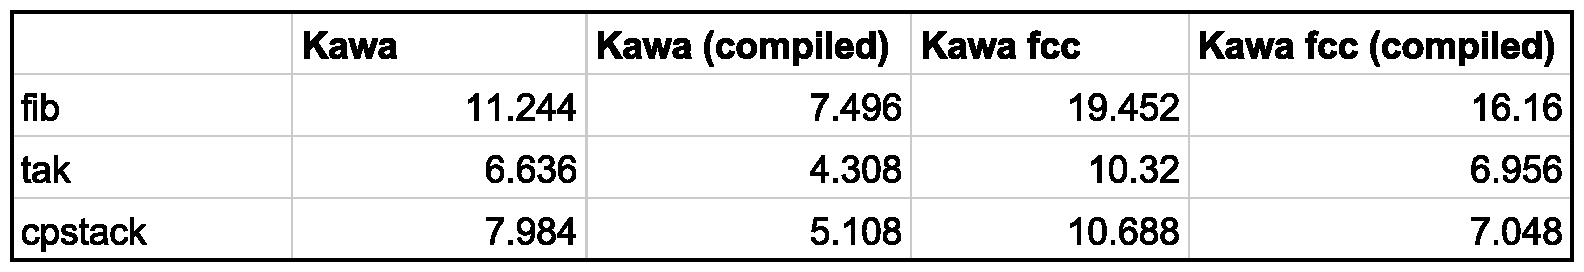
\includegraphics{figures/overhead-table.pdf}
\caption{Transformed vs non-transformed code, 10 iterations, values in
seconds \label{overhead-table}}
\end{figure}

The \texttt{fib} benchmark runs a simple Fibonacci function with 30 as
input. \texttt{tak} implements the Takeuchi function and runs it with
18, 12, 6. \texttt{cpstak} is a version of \texttt{tak} rewritten in
continuation passing style. We can observe that the transformation
introduces a considerable overhead, especially in the \texttt{fib}
benchmark.

\begin{figure}[htbp]
\centering
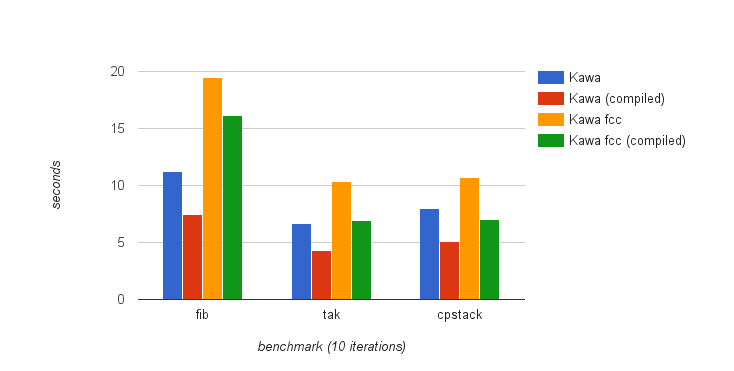
\includegraphics{figures/overhead.png}
\caption{Transformed vs non-transformed code, performance comparison
\label{overhead}}
\end{figure}

To understand from where this overhead comes from, I profiled the
execution of the fib benchmark using HPROF, a profiling tool provided by
the Java platform {[}\hyperref[ref-HPROF2015]{47}{]}. Considering the
cpu usage data (Figure \ref{cpu}), we can observe that approximately
10\% of the cpu time is spent allocating \texttt{Proceure} objects
(\texttt{gnu.mapping.Procedure.\textless{}init\textgreater{}} and
\texttt{gnu.expr.ModuleMethod.\textless{}init\textgreater{}}).

\begin{figure}[htbp]
\centering
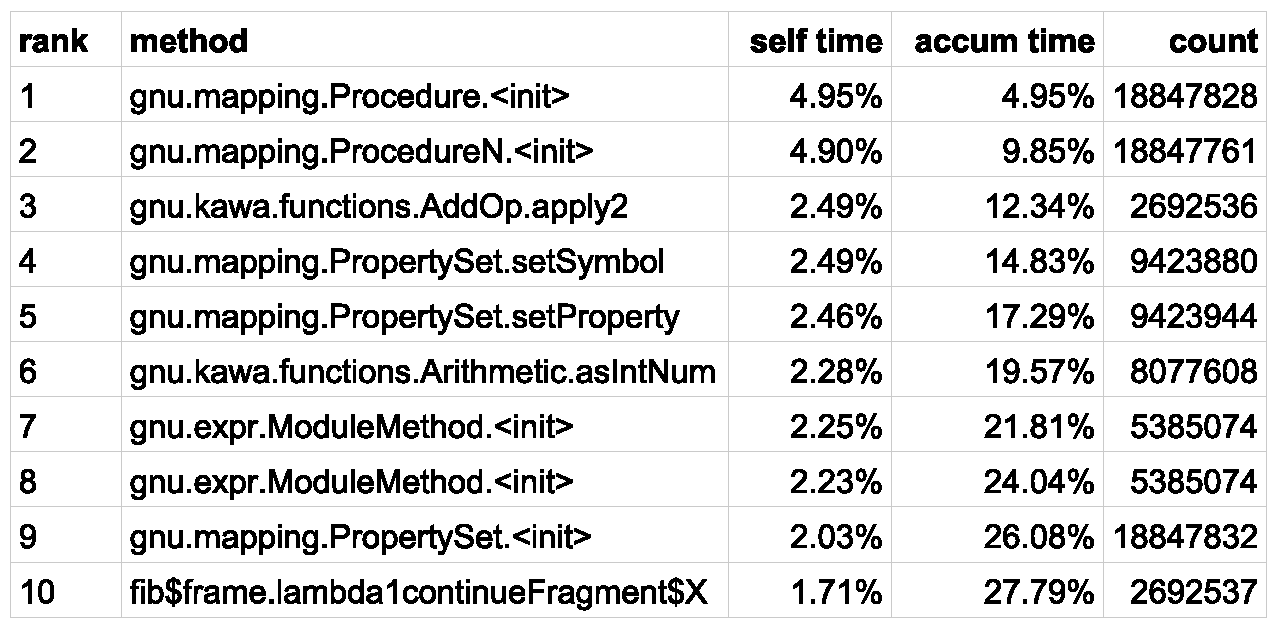
\includegraphics{figures/cpu.pdf}
\caption{Most called Java methods in the \texttt{fib} benchmark
\label{cpu}}
\end{figure}

\begin{figure}[htbp]
\centering
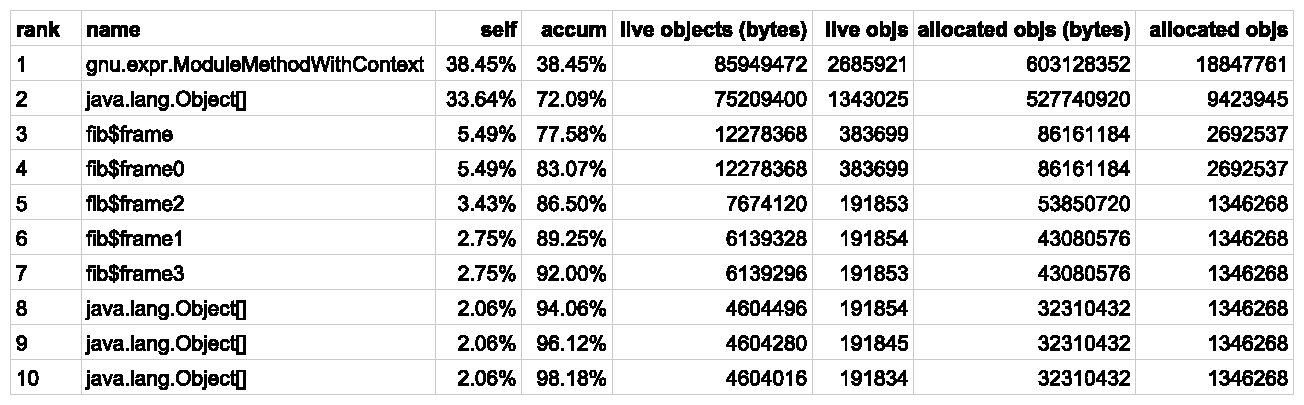
\includegraphics{figures/heap.pdf}
\caption{Most allocated Java object during the execution of the
\texttt{fib} benchmark \label{heap}}
\end{figure}

We can reach the same conclusions analysing the heap usage. Figure
\ref{heap} shows which objects are more often allocated during the
execution of \texttt{fib}.

\begin{figure}[htbp]
\centering
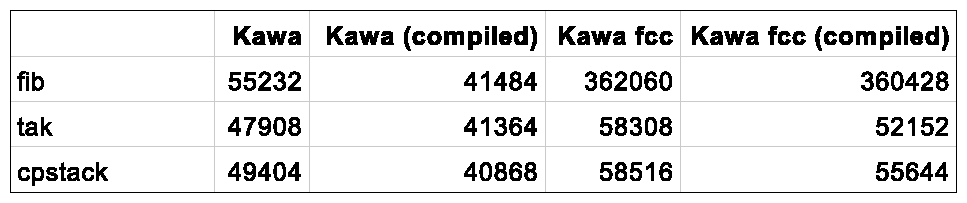
\includegraphics{figures/mem-overhead-table.pdf}
\caption{memory usage in transformed vs non-transformed code, values in
Kbytes \label{mem-overhead-table} \label{heap}}
\end{figure}

Almost 40\% of the heap is used to store object of type
\texttt{ModuleMethodWithContext}, that is the runtime object in which
closures are allocated. This is not unexpected, as the transformed code
is fragmented in a set of closures. However, this suggest that a
possible improvement for the technique can be obtained optimising
closure allocation.

\begin{figure}[htbp]
\centering
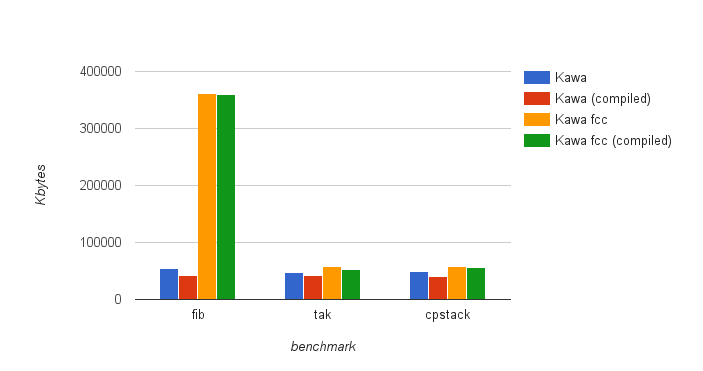
\includegraphics{figures/mem-overhead.png}
\caption{Transformed vs non-transformed code, memory usage comparison
\label{heap}}
\end{figure}

\section{\texorpdfstring{\texttt{call/cc}
performance}{call/cc performance}}\label{callcc-performance}

I tested the new \texttt{call/cc} implementation on five
continuation-intensive benchmarks. \texttt{fibc} is a variation of
\texttt{fib} with continuations. The \texttt{loop2} benchmark
corresponds to a non-local-exit scenario in which a tight loop
repeatedly throws to the same continuation. The \texttt{ctak} benchmark
is a continuation-intensive variation of the call-intensive \texttt{tak}
benchmark. The \texttt{ctak} benchmark captures a continuation on every
procedure call and throws a continuation on every return. In addition to
\texttt{fibc} \texttt{loop2} and \texttt{ctak}, already used in
{[}\hyperref[ref-Clinger1999]{19}{]}, I used a benchmark based on
coroutines, and another implementing a generator.

I compared the modified version of Kawa with other Scheme
implementations with an interpreter or JIT compiler, targeting either
native machine code or an internal VM:

\begin{itemize}
\item
  Petite Chez Scheme is a sibling version of Chez Scheme, a proprietary
  Scheme implementation. Petite is a threaded interpreter and can be
  used free of charge.
\item
  Chicken is a Scheme to C compiler, but also an interpreter.
\item
  Gambit is a Scheme implementation, which has both and interpreter and
  a compiler that produces C code.
\item
  Guile is an interpreter and compiler for Scheme, using a virtual
  machine that executes a portable instruction set generated by its
  optimizing compiler, and integrates very easily with C and C++
  application code.
\item
  Racket is a programming language based on standard Scheme, but
  includes way more features in the base language. It also offers an IDE
  and a large number of built in libraries and tools.
\item
  SISC is a Scheme interpreter written in Java, and running on the JVM.
  SISC is also the only other JVM Scheme supporting \texttt{call/cc}.
\end{itemize}

\begin{figure}[htbp]
\centering
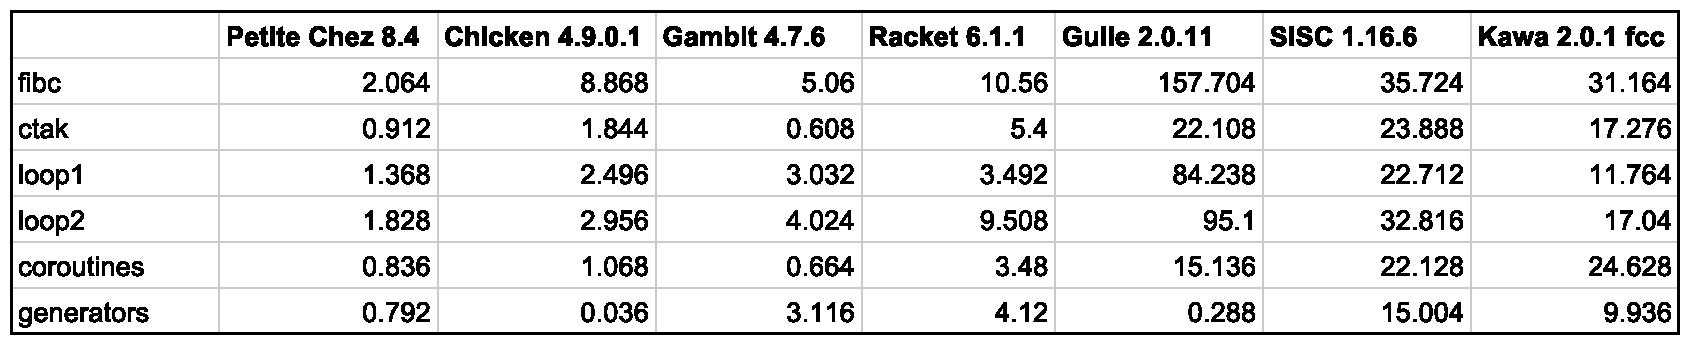
\includegraphics{figures/interpreted-table.pdf}
\caption{Capturing benchmark (interpreted code), 10 iterations, values
in seconds \label{interp-tab}}
\end{figure}

\begin{figure}[htbp]
\centering
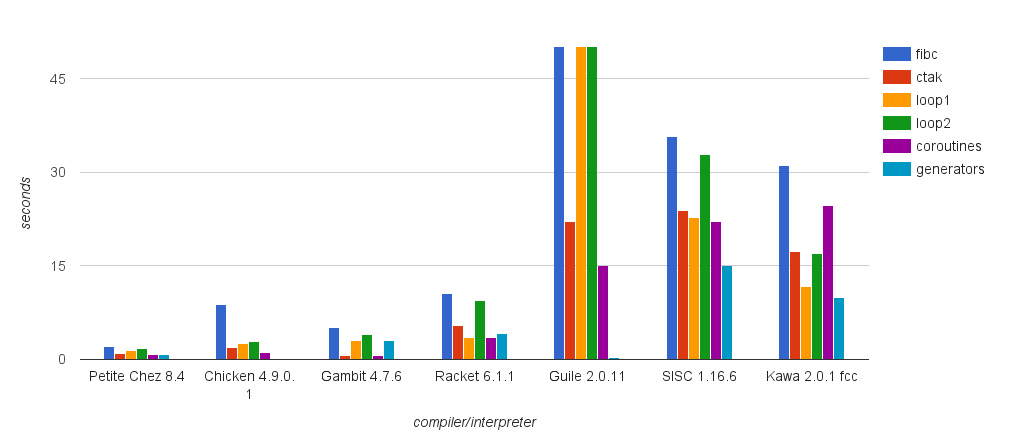
\includegraphics{figures/interpreted.png}
\caption{Capturing benchmark (interpreted code), 10 iterations
\label{interp}}
\end{figure}

Some of the Scheme implementations introduced above can pre-compile code
to a bytecode or binary format, which can be later executed without
paying the cost for translation. Figures \ref{compiled-tab} and
\ref{compiled} compares the execution time of code compiled by five
compilers, including the modified version of Kawa.

\begin{figure}[htbp]
\centering
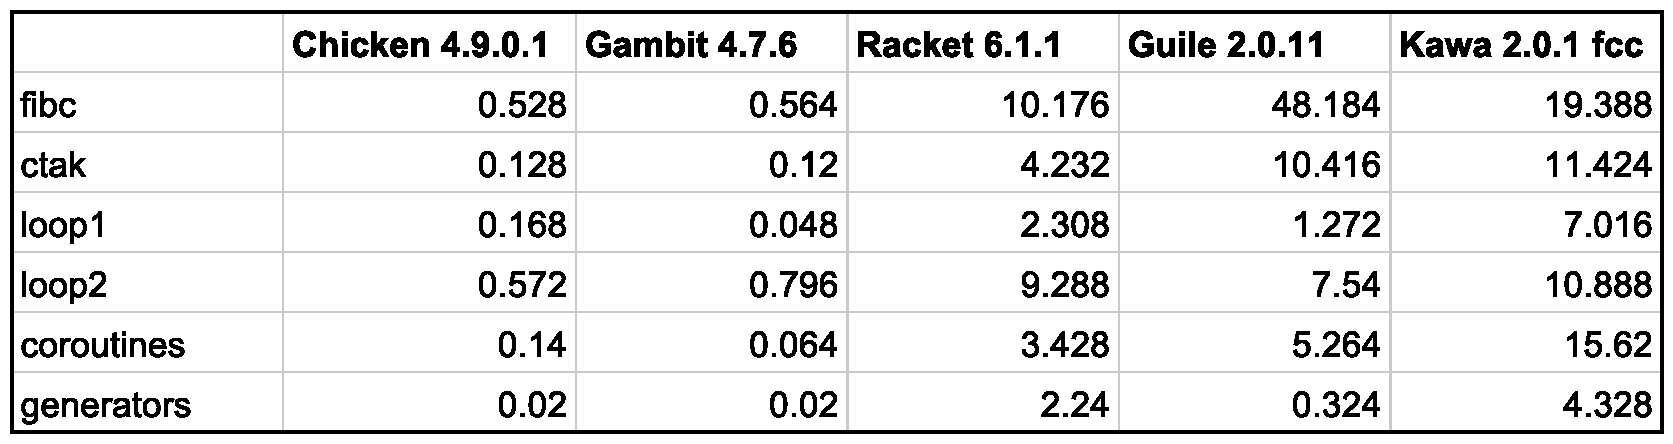
\includegraphics{figures/compiled-table.pdf}
\caption{Capturing benchmark (pre-compiled code), 10 iterations, values
in seconds \label{compiled-tab}}
\end{figure}

\begin{figure}[htbp]
\centering
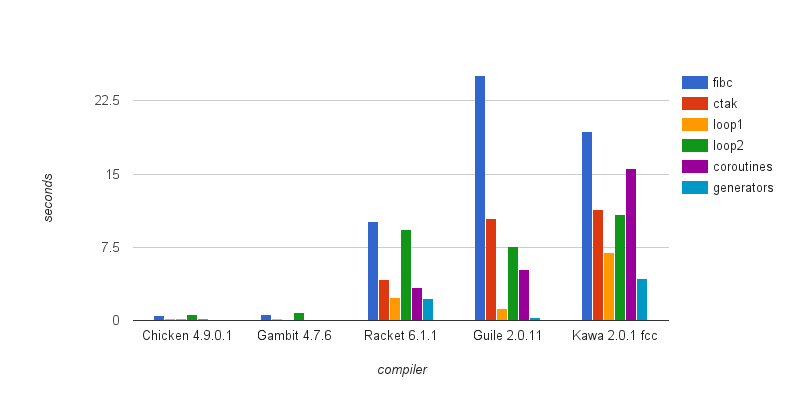
\includegraphics{figures/compiled.png}
\caption{Capturing benchmark (pre-compiled code), 10 iterations
\label{compiled}}
\end{figure}

Looking at the benchmarks' outcome we can see that Kawa with first-class
continuations (Kawa fcc), despite the overhead we measured in the
previous section, performs slightly better then SISC. As expected, Kawa
fcc performances are far from the Scheme to C compilers, however, when
compared with Guile and Racket they are within the same order of
magnitude.

\section{\texorpdfstring{\texttt{call/cc} memory
usage}{call/cc memory usage}}\label{callcc-memory-usage}

I measured peak memory usage of the same five benchmarks introduced in
the performance section, testing the same range of compilers. This time
Kawa fcc performs similarly to SISC, except for the \texttt{fibc}
benchmark. Kawa fcc also uses a similar amount of memory similar to
Racket in the \texttt{coroutines}, \texttt{generators} and \texttt{ctak}
benchmarks. Chez and Scheme to C compilers have performances unreachable
for implementations using a VM, both in interpreted and compiled modes.

\begin{figure}[htbp]
\centering
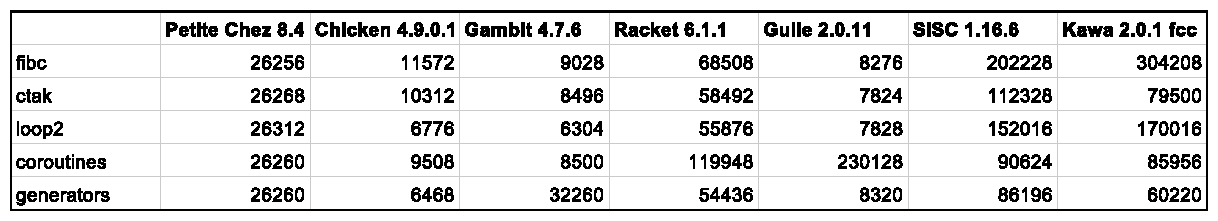
\includegraphics{figures/mem-interpreted-table.pdf}
\caption{Peak memory usage (interpreted code), 10 iterations, values in
Kbytes \label{interp-tab}}
\end{figure}

\begin{figure}[htbp]
\centering
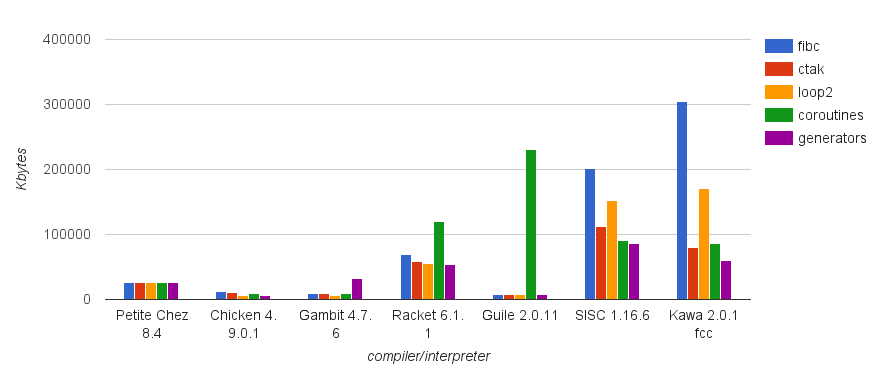
\includegraphics{figures/mem-interpreted.png}
\caption{Peak memory usage (interpreted code), 10 iterations
\label{interp}}
\end{figure}

I repeated the same benchmarks using pre-compiled code. However, with
relation to memory usage, the differences between interpreted vs
compiled code is negligible.

\begin{figure}[htbp]
\centering
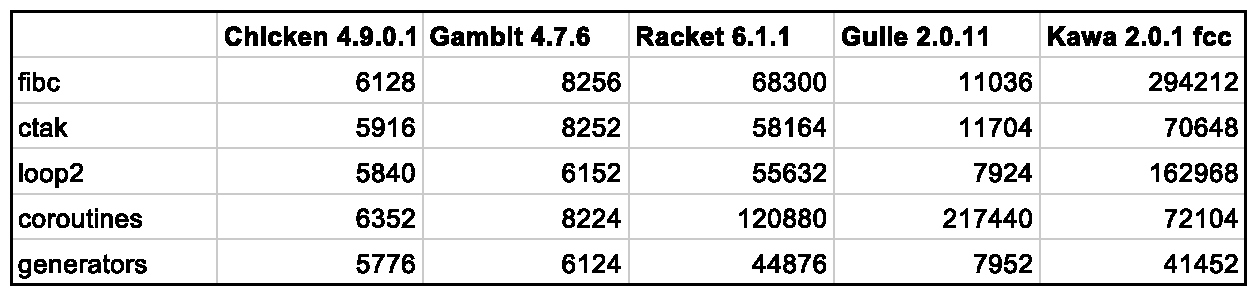
\includegraphics{figures/mem-compiled-table.pdf}
\caption{Peak memory usage (pre-compiled code), 10 iterations, values in
Kbytes \label{compiled-tab}}
\end{figure}

\begin{figure}[htbp]
\centering
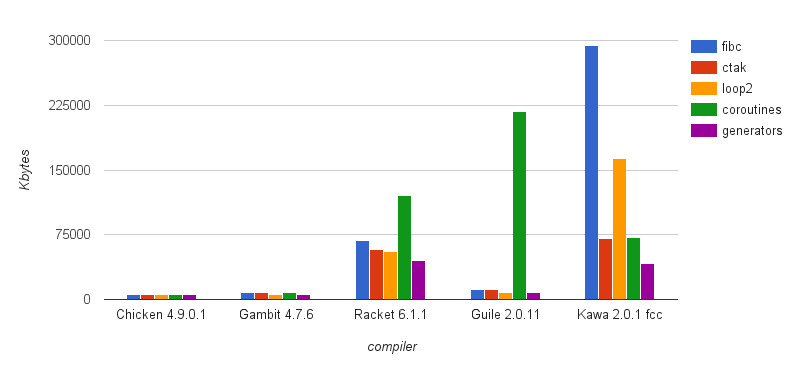
\includegraphics{figures/mem-compiled.png}
\caption{Peak memory usage (pre-compiled code), 10 iterations
\label{compiled}}
\end{figure}

\section{Code size}\label{code-size-1}

We saw in Chapter 3 that we expect an increase in code size proportional
to the number of code fragments, so we want to measure the actual
difference in size between a regular class file and an instrumented one.
Figure \ref{codesize-tab} shows a comparison of regular code and
transformed code.

\begin{figure}[htbp]
\centering
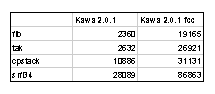
\includegraphics{figures/codesize-table.pdf}
\caption{Code size comparison, values in bytes \label{codesize-tab}}
\end{figure}

We can observe that the size of transformed code can be 10 times larger
than the code compiled without first-class continuations enabled. Even
if the code size increase is proportional to the number of fragments,
the difference in size is significant. This indicates that would be
better to limit the use of transformed code to modules that needs
\texttt{call/cc}, and use \texttt{call/cc} enabled code in combination
with non-transformed code.

\begin{figure}[htbp]
\centering
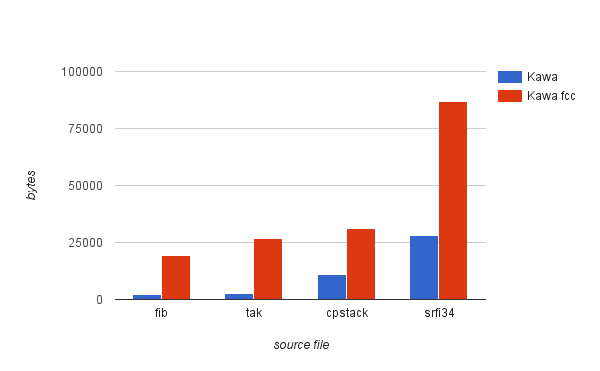
\includegraphics{figures/codesize.png}
\caption{Size of compiled classes in bytes \label{codesize}}
\end{figure}

\chapter{Conclusions and future work}\label{conclusions-and-future-work}

This dissertation has presented an implementation of the
\texttt{call/cc} control operator in Kawa, a Scheme compiler targeting
the JVM. Although the problem was delineated in some works in
literature, there was not a compiler providing first-class continuations
on the JVM in terms of \texttt{call/cc}.

I developed a variant of generalised stack inspection in the Kawa
compiler, addressing the problem of defining an A-normalisation
algorithm for the Kawa super-set of Scheme, and realising a
fragmentation and instrumentation pass using the existing Kawa
framework. The whole transformation has been designed to be optional and
separated from the existing passes, so that it does not add unnecessary
overhead to modules without continuations.

I explored variations of the technique to implement other control
operators, such as \texttt{shift}/\texttt{reset} and prompts, as well as
continuation barriers. Moreover, the two passes are flexible enough that
could be used on a portion of the syntax tree, instead of the entire
program.

I showed the opportunities opened by the availability of
\texttt{call/cc}, developing a syntax for asynchronous programming, and
exploiting the A-normalisation of the syntax tree to create a simple
debugger.

The evaluation of performance and memory usage revealed that this
technique can be a valid alternative to heap-based implementations of
\texttt{call/cc}. Benchmarks also showed that the bottleneck of the
technique is not exception handling, but closure allocation, leaving
room for improvement.

\section{Future work}\label{future-work}

This work can be further developed in several interesting directions. I
will outline a few possible applications and extensions, which can be
based on this contribution to implement new features and obtain
improvements in other programming languages or framework.

\begin{itemize}
\item
  Variants of this technique can be employed in other JVM languages to
  implement first-class delimited and un-delimited continuations and
  control operators. Languages like Clojure, JRuby, Groovy, Bigloo and
  others could take advantage of this work.
\item
  The transformation described in the previous pages uses an
  intermediate A-normalisation pass. ANF has been related in other works
  to Static Single Assignment (SSA) form
  {[}\hyperref[ref-Chakravarty2004]{48}{]}. It is possible to exploit
  the formal properties of ANF to implement in the compiler many
  optimisation present in literature.
\item
  In the past few years several frameworks for concurrency appeared on
  the Java scene. Many of them use bytecode instrumentation to implement
  coroutines and provide lightweight threads with low memory and
  task-switching overhead. Quasar
  {[}\hyperref[ref-QuasarAkka2015]{49}{]}, for instance, deliver the
  actor model on the JVM using bytecode instrumentation. The
  transformation presented in this document can give an alternative for
  those frameworks that aim to provide a concurrency API for Java or JVM
  languages.
\item
  Research has been done on the use of continuations in the context of
  web applications {[}\hyperref[ref-Matthews2004]{50},
  \hyperref[ref-Queinnec2004]{51}{]}. The support for first-class
  continuations developed in the context of this thesis, can be utilised
  to implement continuation based web frameworks in Kawa or in Java.
\item
  The research field of Dynamic Software Updating (DSU) pertains to
  upgrading programs while they are running
  {[}\hyperref[ref-gregersen2014state]{52},
  \hyperref[ref-Makris2009]{53}{]}. Different approaches for DSU has
  been developed, nevertheless it is not currently widely used in
  industry. Some of the approaches use a stack reconstruction technique
  similar in many aspects to the \texttt{call/cc} implementation
  described in this dissertation {[}\hyperref[ref-Buisson2008]{54}{]}.
  Future work can start from the achievements of this work to explore an
  alternative implementation of DSU on the JVM.
\end{itemize}

\backmatter

\chapter*{References}\label{references}
\addcontentsline{toc}{chapter}{References}

{\setstretch{1.2} \setlength{\parskip}{2em}
\hyperdef{}{ref-TurnConcurrency2015}{\label{ref-TurnConcurrency2015}}
{[}1{]} H. Sutter, ``The Free Lunch Is Over: A Fundamental Turn Toward
Concurrency in Software.'' {[}Online{]}. Available:
\url{http://www.gotw.ca/publications/concurrency-ddj.htm}. {[}Accessed:
14-Jun-2015{]}

\hyperdef{}{ref-TIOBEIndex2015}{\label{ref-TIOBEIndex2015}}
{[}2{]} ``TIOBE Software: Tiobe Index.'' {[}Online{]}. Available:
\url{http://www.tiobe.com/index.php/content/paperinfo/tpci/index.html}.
{[}Accessed: 11-Jun-2015{]}

\hyperdef{}{ref-JavaWiki2015}{\label{ref-JavaWiki2015}}
{[}3{]} ``Java (programming language) - Wikipedia, the free
encyclopedia.'' {[}Online{]}. Available:
\url{https://en.wikipedia.org/wiki/Java_(programming_language)}.
{[}Accessed: 13-Jun-2015{]}

\hyperdef{}{ref-OracleLambda2015}{\label{ref-OracleLambda2015}}
{[}4{]} ``Lambda Expressions (The Java™ Tutorials).'' Oracle
{[}Online{]}. Available:
\url{https://docs.oracle.com/javase/tutorial/java/javaOO/lambdaexpressions.html}.
{[}Accessed: 15-Jun-2015{]}

\hyperdef{}{ref-WhyLambda2013}{\label{ref-WhyLambda2013}}
{[}5{]} M. Fusco, ``Why We Need Lambda Expressions in Java \textbar{}
Javalobby.'' 27-Mar-2013 {[}Online{]}. Available:
\url{http://java.dzone.com/articles/why-we-need-lambda-expressions}.
{[}Accessed: 13-Jun-2015{]}

\hyperdef{}{ref-JVMWiki2015}{\label{ref-JVMWiki2015}}
{[}6{]} ``Java virtual machine - Wikipedia, the free encyclopedia.''
{[}Online{]}. Available:
\url{https://en.wikipedia.org/wiki/Java_virtual_machine}. {[}Accessed:
13-Jun-2015{]}

\hyperdef{}{ref-JVMLang2015}{\label{ref-JVMLang2015}}
{[}7{]} ``Alternative Languages for the JVM.'' {[}Online{]}. Available:
\url{http://www.oracle.com/technetwork/articles/java/architect-languages-2266279.html}.
{[}Accessed: 14-Jun-2015{]}

\hyperdef{}{ref-SchemeWiki2015}{\label{ref-SchemeWiki2015}}
{[}8{]} ``Scheme (programming language) - Wikipedia, the free
encyclopedia.'' {[}Online{]}. Available:
\url{https://en.wikipedia.org/wiki/Scheme_(programming_language)}.
{[}Accessed: 15-Jun-2015{]}

\hyperdef{}{ref-dybvig2009scheme}{\label{ref-dybvig2009scheme}}
{[}9{]} R. K. Dybvig, \emph{The Scheme programming language, Fourth
Edition}. 2009 {[}Online{]}. Available:
\url{http://www.scheme.com/tspl4/}

\hyperdef{}{ref-dybvig1987three}{\label{ref-dybvig1987three}}
{[}10{]} R. K. Dybvig, ``Three implementation models for scheme,''
PhD thesis, University of North Carolina at Chapel Hill, 1987
{[}Online{]}. Available:
\url{http://www.cs.indiana.edu/~dyb/pubs/3imp.pdf}

\hyperdef{}{ref-ContByExample2015}{\label{ref-ContByExample2015}}
{[}11{]} M. Might, ``Continuations by example.'' {[}Online{]}.
Available: \url{http://goo.gl/ECRA5r}. {[}Accessed: 15-Jun-2015{]}

\hyperdef{}{ref-WhyContCool2015}{\label{ref-WhyContCool2015}}
{[}12{]} D. Martins, ``Why Are Continuations So Darn Cool?''
{[}Online{]}. Available:
\url{http://danielmartins.ninja/posts/why-are-continuations-so-darn-cool.html}.
{[}Accessed: 15-Jun-2015{]}

\hyperdef{}{ref-PageCallcc2015}{\label{ref-PageCallcc2015}}
{[}13{]} D. Madore, ``A page about call/cc.'' {[}Online{]}. Available:
\url{http://www.madore.org/~david/computers/callcc.html}. {[}Accessed:
15-Jun-2015{]}

\hyperdef{}{ref-Asai2011}{\label{ref-Asai2011}}
{[}14{]} K. Asai and O. Kiselyov, \emph{Introduction to Programming with
Shift and Reset}. 2011 {[}Online{]}. Available:
\url{http://www.is.ocha.ac.jp/~asai/cw2011tutorial/main-e.pdf}

\hyperdef{}{ref-kiselyov2007delimited}{\label{ref-kiselyov2007delimited}}
{[}15{]} O. Kiselyov and C.-c. Shan, ``Delimited continuations in
operating systems,'' in \emph{Modeling and Using Context}, Springer,
2007, pp. 291--302 {[}Online{]}. Available:
\url{http://www.okmij.org/ftp/continuations/ZFS/context-OS.pdf}

\hyperdef{}{ref-RacketContinuations2015}{\label{ref-RacketContinuations2015}}
{[}16{]} ``Continuations - Racket Documentation.'' {[}Online{]}.
Available:
\url{http://docs.racket-lang.org/reference/cont.html\#(part._.Classical_.Control_.Operators)}.
{[}Accessed: 14-Jun-2015{]}

\hyperdef{}{ref-DelimitedWiki2015}{\label{ref-DelimitedWiki2015}}
{[}17{]} ``Delimited continuation - Wikipedia, the free encyclopedia.''
{[}Online{]}. Available:
\url{https://en.wikipedia.org/wiki/Delimited_continuation}. {[}Accessed:
14-Jun-2015{]}

\hyperdef{}{ref-Kawa2015}{\label{ref-Kawa2015}}
{[}18{]} ``Kawa: The Kawa Scheme language.'' {[}Online{]}. Available:
\url{http://www.gnu.org/software/kawa/index.html}. {[}Accessed:
15-Jun-2015{]}

\hyperdef{}{ref-Clinger1999}{\label{ref-Clinger1999}}
{[}19{]} W. D. Clinger, A. H. Hartheimer, and E. M. Ost,
``Implementation strategies for first-class continuations,''
\emph{Higher-Order and Symbolic Computation}, vol. 12, no. 1, pp. 7--45,
1999 {[}Online{]}. Available:
\url{http://link.springer.com/article/10.1023/A:1010016816429}

\hyperdef{}{ref-Miller2002}{\label{ref-Miller2002}}
{[}20{]} S. G. Miller, ``SISC: A complete scheme interpreter in java,''
Technical Report, Jan, 2002 {[}Online{]}. Available:
\url{http://sisc-scheme.org/sisc.pdf}

\hyperdef{}{ref-appel2006compiling}{\label{ref-appel2006compiling}}
{[}21{]} A. W. Appel, \emph{Compiling with continuations}. Cambridge
University Press, 2006.

\hyperdef{}{ref-adams1986orbit}{\label{ref-adams1986orbit}}
{[}22{]} N. Adams, D. Kranz, R. Kelsey, J. Rees, P. Hudak, and J.
Philbin, \emph{Orbit: An optimizing compiler for Scheme}, vol. 21. ACM,
1986 {[}Online{]}. Available:
\url{http://dl.acm.org/citation.cfm?id=13333}

\hyperdef{}{ref-Rompf2009}{\label{ref-Rompf2009}}
{[}23{]} T. Rompf, I. Maier, and M. Odersky, ``Implementing first-class
polymorphic delimited continuations by a type-directed selective
CPS-transform,'' in \emph{Proceedings of the 14th ACM SIGPLAN
international conference on Functional programming - ICFP '09}, 2009, p.
317 {[}Online{]}. Available:
\url{http://dl.acm.org/citation.cfm?doid=1596550.1596596}

\hyperdef{}{ref-McBeath2010}{\label{ref-McBeath2010}}
{[}24{]} J. McBeath, ``Delimited Continuations.'' August-2010
{[}Online{]}. Available:
\url{http://jim-mcbeath.blogspot.co.uk/2010/08/delimited-continuations.html}

\hyperdef{}{ref-Pettyjohn2005}{\label{ref-Pettyjohn2005}}
{[}25{]} G. Pettyjohn, J. Clements, J. Marshall, S. Krishnamurthi, and
M. Felleisen, ``Continuations from generalized stack inspection,'' in
\emph{Proceedings of the tenth ACM SIGPLAN international conference on
Functional programming - ICFP '05}, 2005, p. 216 {[}Online{]}.
Available: \url{http://portal.acm.org/citation.cfm?doid=1086365.1086393}

\hyperdef{}{ref-Sekiguchi2001}{\label{ref-Sekiguchi2001}}
{[}26{]} T. Sekiguchi, T. Sakamoto, and A. Yonezawa, ``Advances in
Exception Handling Techniques,'' A. Romanovsky, C. Dony, J. L. Knudsen,
and A. Tripathi, Eds. Springer Berlin Heidelberg, 2001, pp. 217--233
{[}Online{]}. Available:
\url{http://dx.doi.org/10.1007/3-540-45407-1_14}

\hyperdef{}{ref-tao2001portable}{\label{ref-tao2001portable}}
{[}27{]} W. Tao, ``A portable mechanism for thread persistence and
migration,'' PhD thesis, School of Computing, University of Utah, 2001
{[}Online{]}. Available: \url{http://www.cs.utah.edu/~tao/research/}

\hyperdef{}{ref-Loitsch2007}{\label{ref-Loitsch2007}}
{[}28{]} F. Loitsch, \emph{Exceptional continuations in JavaScript}.
2007 {[}Online{]}. Available:
\url{http://repository.readscheme.org/ftp/papers/sw2007/04-loitsch.pdf}

\hyperdef{}{ref-Marshall2009}{\label{ref-Marshall2009}}
{[}29{]} J. Marshall, ``An Unexceptional Implementation of First-Class
Continuations,'' in \emph{Proceedings of the 2009 International Lisp
Conference}, 2009, pp. 36--40 {[}Online{]}. Available:
\url{https://drive.google.com/file/d/0B4zj6rF-PmISMTNjYWVhYmYtZTQ1MC00YTg4LWFiYTQtYzJiZjQwMzQyMjA1/view?ddrp=1\&hl=en}

\hyperdef{}{ref-Srinivasan2006}{\label{ref-Srinivasan2006}}
{[}30{]} S. Srinivasan, \emph{A thread of one's own}, vol. 4. 2006
{[}Online{]}. Available:
\url{http://malhar.net/sriram/kilim/thread_of_ones_own.pdf}

\hyperdef{}{ref-Bolton2000}{\label{ref-Bolton2000}}
{[}31{]} L. Bolton, ``Kilim: a server framework with lightweight actors,
isolation types, and zero-copy messaging,'' \emph{The Contemporary
Pacific}, vol. 12, no. 2, pp. 561--563, 2000 {[}Online{]}. Available:
\url{http://muse.jhu.edu/content/crossref/journals/contemporary/_pacific/v012/12.2bolton.html}

\hyperdef{}{ref-StackHack2005}{\label{ref-StackHack2005}}
{[}32{]} G. Pettyjohn, J. Clements, J. Marshall, S. Krishnamurthi, and
M. Felleisen, ``A Technique for Implementing First-Class
Continuations.'' 2005 {[}Online{]}. Available:
\url{http://www.ccs.neu.edu/racket/pubs/stackhack4.html}

\hyperdef{}{ref-Longjumps2015}{\label{ref-Longjumps2015}}
{[}33{]} J. Rose, ``Longjumps Considered Inexpensive.'' 10-May-2007
{[}Online{]}. Available:
\url{https://blogs.oracle.com/jrose/entry/longjumps_considered_inexpensive}.
{[}Accessed: 09-Jun-2015{]}

\hyperdef{}{ref-Flanagan1993}{\label{ref-Flanagan1993}}
{[}34{]} C. Flanagan, A. Sabry, B. F. Duba, and M. Felleisen, ``The
essence of compiling with continuations,'' in \emph{Proceedings of the
ACM SIGPLAN 1993 conference on Programming language design and
implementation - PLDI '93}, 1993, pp. 237--247 {[}Online{]}. Available:
\url{http://portal.acm.org/citation.cfm?doid=155090.155113}

\hyperdef{}{ref-Javaflow2015}{\label{ref-Javaflow2015}}
{[}35{]} ``Commons Javaflow - Overview.'' {[}Online{]}. Available:
\url{http://commons.apache.org/sandbox/commons-javaflow/}. {[}Accessed:
09-Jun-2015{]}

\hyperdef{}{ref-Stadler2009}{\label{ref-Stadler2009}}
{[}36{]} L. Stadler, C. Wimmer, T. Würthinger, H. Mössenböck, and J.
Rose, ``Lazy continuations for Java virtual machines,'' in
\emph{Proceedings of the 7th International Conference on Principles and
Practice of Programming in Java - PPPJ '09}, 2009, p. 143 {[}Online{]}.
Available: \url{http://portal.acm.org/citation.cfm?doid=1596655.1596679}

\hyperdef{}{ref-RIFE2015}{\label{ref-RIFE2015}}
{[}37{]} ``RIFE : About.'' {[}Online{]}. Available:
\url{http://rifers.org/}. {[}Accessed: 09-Jun-2015{]}

\hyperdef{}{ref-begel2000picothreads}{\label{ref-begel2000picothreads}}
{[}38{]} A. Begel, J. MacDonald, and M. Shilman, ``PicoThreads:
Lightweight threads in Java,'' \emph{Department of Electrical
Engineering \& Computer Sciences University of California, Berkeley},
2000 {[}Online{]}. Available:
\url{http://research.microsoft.com/en-us/um/people/abegel/cs262/picothreads.pdf}

\hyperdef{}{ref-ContinuationsLib2015}{\label{ref-ContinuationsLib2015}}
{[}39{]} M. Mann, ``Continuations Library.'' {[}Online{]}. Available:
\url{http://www.matthiasmann.de/content/view/24/26/}. {[}Accessed:
09-Jun-2015{]}

\hyperdef{}{ref-Bothner1998}{\label{ref-Bothner1998}}
{[}40{]} P. Bothner, ``Kawa internals: Compiling Scheme to Java.''
17-November-1998 {[}Online{]}. Available:
\url{http://www.gnu.org/software/kawa/internals/index.html}

\hyperdef{}{ref-ANFMight2015}{\label{ref-ANFMight2015}}
{[}41{]} M. Might, ``A-Normalization: Why and How.'' {[}Online{]}.
Available: \url{http://matt.might.net/articles/a-normalization/}.
{[}Accessed: 17-Jun-2015{]}

\hyperdef{}{ref-jmh2015}{\label{ref-jmh2015}}
{[}42{]} ``OpenJDK: jmh.'' {[}Online{]}. Available:
\url{http://openjdk.java.net/projects/code-tools/jmh/}. {[}Accessed:
23-Jun-2015{]}

\hyperdef{}{ref-BenchmarkingJVM2015}{\label{ref-BenchmarkingJVM2015}}
{[}43{]} J. Ponge, ``Avoiding Benchmarking Pitfalls on the JVM.''
{[}Online{]}. Available:
\url{http://www.oracle.com/technetwork/articles/java/architect-benchmarking-2266277.html}.
{[}Accessed: 23-Jun-2015{]}

\hyperdef{}{ref-EvaluationRacket2015}{\label{ref-EvaluationRacket2015}}
{[}44{]} ``1.1 Evaluation Model.'' {[}Online{]}. Available:
\url{http://docs.racket-lang.org/reference/eval-model.html\#\%28part._prompt-model\%29}.
{[}Accessed: 28-Jun-2015{]}

\hyperdef{}{ref-Filinski1994}{\label{ref-Filinski1994}}
{[}45{]} A. Filinski, ``Representing monads,'' in \emph{Proceedings of
the 21st ACM SIGPLAN-SIGACT symposium on Principles of programming
languages - POPL '94}, 1994, pp. 446--457 {[}Online{]}. Available:
\url{http://portal.acm.org/citation.cfm?doid=174675.178047}

\hyperdef{}{ref-biagioni1998safe}{\label{ref-biagioni1998safe}}
{[}46{]} E. Biagioni, K. Cline, P. Lee, C. Okasaki, and C. Stone,
``Safe-for-space threads in Standard ML,'' \emph{Higher-Order and
Symbolic Computation}, vol. 11, no. 2, pp. 209--225, 1998 {[}Online{]}.
Available:
\url{http://link.springer.com/article/10.1023/A:1010016600604}

\hyperdef{}{ref-HPROF2015}{\label{ref-HPROF2015}}
{[}47{]} ``HPROF: A Heap/CPU Profiling Tool.'' Oracle {[}Online{]}.
Available:
\url{http://docs.oracle.com/javase/8/docs/technotes/samples/hprof.html}.
{[}Accessed: 26-Jun-2015{]}

\hyperdef{}{ref-Chakravarty2004}{\label{ref-Chakravarty2004}}
{[}48{]} M. M. Chakravarty, G. Keller, and P. Zadarnowski, ``A
Functional Perspective on SSA Optimisation Algorithms,''
\emph{Electronic Notes in Theoretical Computer Science}, vol. 82, no. 2,
pp. 347--361, Apr 2004 {[}Online{]}. Available:
\url{http://dx.doi.org/10.1016/S1571-0661(05)82596-4}

\hyperdef{}{ref-QuasarAkka2015}{\label{ref-QuasarAkka2015}}
{[}49{]} ``Parallel Universe.'' Parallel Universe {[}Online{]}.
Available:
\url{http://blog.paralleluniverse.co/2015/05/21/quasar-vs-akka/}.
{[}Accessed: 29-Jun-2015{]}

\hyperdef{}{ref-Matthews2004}{\label{ref-Matthews2004}}
{[}50{]} J. Matthews, R. B. Findler, P. Graunke, S. Krishnamurthi, and
M. Felleisen, ``Automatically Restructuring Programs for the Web,''
\emph{Automated Software Engineering}, vol. 11, no. 4, pp. 337--364, Oct
2004 {[}Online{]}. Available:
\url{http://dx.doi.org/10.1023/B:AUSE.0000038936.09009.69}

\hyperdef{}{ref-Queinnec2004}{\label{ref-Queinnec2004}}
{[}51{]} C. Queinnec, ``Continuations and Web Servers,'' vol. 17, no. 4,
pp. 277--295, Dec 2004 {[}Online{]}. Available:
\url{http://dx.doi.org/10.1007/s10990-004-4866-z}

\hyperdef{}{ref-gregersen2014state}{\label{ref-gregersen2014state}}
{[}52{]} A. R. Gregersen, M. Rasmussen, and B. N. Jørgensen, ``State of
the Art of Dynamic Software Updating in Java,'' in \emph{Software
Technologies}, Springer, 2014, pp. 99--113 {[}Online{]}. Available:
\url{http://link.springer.com/chapter/10.1007\%2F978-3-662-44920-2_7}

\hyperdef{}{ref-Makris2009}{\label{ref-Makris2009}}
{[}53{]} K. Makris and R. A. Bazzi, \emph{Immediate Multi-Threaded
Dynamic Software Updates Using Stack Reconstruction.}, vol. 2009. 2009
{[}Online{]}. Available:
\url{http://static.usenix.org/legacy/events/usenix09/tech/full_papers/makris/makris.pdf}

\hyperdef{}{ref-Buisson2008}{\label{ref-Buisson2008}}
{[}54{]} J. Buisson and F. Dagnat, ``Introspecting continuations in
order to update active code,'' in \emph{Proceedings of the 1st
International Workshop on Hot Topics in Software Upgrades - HotSWUp
'08}, 2008, p. 1 {[}Online{]}. Available:
\url{http://portal.acm.org/citation.cfm?doid=1490283.1490289}
}

\end{document}
